\documentclass[11pt]{amsart}

\usepackage{graphicx,amsmath,amssymb,amsthm,bbm,url}
\usepackage{algorithm,algorithmic,caption,subcaption}
\usepackage{fullpage}
\usepackage{color,arydshln,verbatim}
\usepackage[dvipsnames]{xcolor}

\newcommand{\RSnote}[1]{\textcolor{blue}{[{\em {\bf **RS Note:} #1}]}}
\newcommand{\MIAnote}[1]{\textcolor{red}{[{\em {\bf **MIA Note:} #1}]}}
\newcommand{\BPnote}[1]{\textcolor{ForestGreen}{[{\em {\bf **BP Note:} #1}]}}
\newtheorem{lem}{Lemma}
\newtheorem{cor}{Corollary}
\newtheorem{thm}{Theorem}
\newtheorem{Def}{Definition}
\newtheorem{prop}{Proposition}
%\renewcommand{\baselinestretch}{1.25}

\DeclareMathOperator{\supp}{supp}

\def \a {\mathbf a}
\def \b {\mathbf b}
\def \x {\mathbf x}
\def \z {\mathbf z}
\def \y {\mathbf y}
\def \u {\mathbf u}
\def \v {\mathbf v}
\def \X { X}
\def \Y { Y}
\def \m {\mathbf m}
\def \n {\mathbf n}
\newcommand{\R}{\ensuremath{\mathbb{R}}}  % The real numbers.
\newcommand{\Z}{\ensuremath{\mathbb{Z}}}  % The integers
\renewcommand{\H}{\ensuremath{\mathcal{H}}}
\newcommand{\tX}{\ensuremath{\widetilde{X}}}
\newcommand{\tD}{\ensuremath{\tilde{D}}}
\newcommand{\tx}{\ensuremath{\widetilde{\x}}}
\newcommand{\C}{\ensuremath{\mathbb{C}}}
\newcommand{\N}{\ensuremath{\mathbb{N}}}
\newcommand{\Rn}{\ensuremath{\R^n}}
\newcommand{\Cn}{\ensuremath{\C^n}}
\newcommand{\bigfrac}[2]{\ensuremath{\frac{\displaystyle #1}{\displaystyle #2}}}
\newcommand{\Span}{\ensuremath{\mathrm{span}}}
\newcommand{\Nul}{\ensuremath{\mathrm{Null}}}
\newcommand{\Tr}{\ensuremath{\mathrm{Tr}}}
\newcommand{\ee}{\ensuremath{\mathbbm{e}}}
\newcommand{\ii}{\ensuremath{\mathbbm{i}}}
\newcommand{\diag}{\ensuremath{\mathrm{diag}}}
\newcommand{\sgn}{\ensuremath{\mathrm{sgn}}}
\newcommand{\vol}{\ensuremath{\mathrm{vol}}}
%\newcommand{\Re}{\ensuremath{\mathrm{Re}}}
%\newcommand{\Im}{\ensuremath{\mathrm{Im}}}


% Use more than 10 columns in bmatrix
\setcounter{MaxMatrixCols}{20}

% Reduce space between columns (for use with bmatrix and the 
% block circulant system matrix definition)
\def\SmallColSep{\setlength{\arraycolsep}{0.8\arraycolsep}}

\begin{document}
\pagestyle{plain}


\title{Phase Retrieval from Local Measurements:  Improved Robustness via Eigenvector-Based Angular
Synchronization}\thanks{Mark A. Iwen:  Department of Mathematics, and Department of Computational
Mathematics, Science, and Engineering (CMSE), Michigan State University, East Lansing, MI, 48824,
USA (markiwen@math.msu.edu).   \\ \indent B. Preskitt:  Department of Mathematics, University of
California San Diego, La Jolla, CA 92093, USA (bpreskitt@ucsd.edu)\\ \indent  R. Saab:  Department
of Mathematics, University of California San Diego, La Jolla, CA 92093, USA (rsaab@ucsd.edu).   \\
\indent A. Viswanathan:  Department of Mathematics and Statistics, University of Michigan --
Dearborn, Dearborn, MI, 48128, USA (adityavv@umich.edu).}
\author{Mark A. Iwen, Brian Preskitt, Rayan Saab, Aditya Viswanathan}
%\date{April 23, 2015}

%\date{April 23, 2015}

\begin{abstract}%\RSnote{rewrite}
%We propose a new phase retrieval approach for correlation-based measurements with compactly supported measurement masks.  Lifting based (discuss...) -- improved theoretical as well as numerical robustness results are demonstrated.  In addition, the method is fast, outperforming standard approaches such as PhaseLift and WirtingerFlow with respect to computational complexity(CHECK THAT -- need to show we can beat WTF). Finally, it is shown that the proposed phase retrieval approach for correlation-based measurements also trivially extends to allow phase retrieval for STFT measurements.
In this dissertation, we study a new approach to the problem of phase retrieval, which is the task of reconstructing a complex-valued signal from magnitude-only measurements.  This problem occurs naturally in several specialized imaging applications such as electron microscopy and X-ray crystallography.  Although solutions were first proposed for this problem as early as the 1970s, these algorithms have lacked theoretical guarantees of success, and phase retrieval has suffered from a considerable gap between practice and theory for almost the entire history of its study.

A common technique in fields that use phase retrieval is that of \emph{ptychography}, where measurements are collected by only illuminating small sections of the sample at any time.  We refer to measurements designed in this way as \emph{local measurements}, and in this dissertation, we develop and expand the theory for solving phase retrieval in measurement regimes of this kind.  Our first contribution is a basic model for this setup in the case of a one-dimensional signal, along with an algorithm that robustly solves phase retrieval under this model.  This work is unique in many ways that represent substantial improvements over previously existing solutions: perhaps most significantly, many of the recovery guarantees in recent work rely on the measurements being generated by a random process, while we devise a class of measurements for which the conditioning of the system is known and quickly checkable (see \cref{sec:con_number}).  These advantages constitute major progress towards producing theoretical results for phase retrieval that are directly usable in laboratory settings.

Chapter 1 conducts a survey of the history of phase retrieval and its applications.  Chapter 2 reviews the mathematical literature on the subject, including the first solutions and the theoretical work of the last decade.  Chapter 3 presents co-authored results defining and establishing the setting and solution of the base model explored in this dissertation.  Chapter 4 expands the theory on what measurement schemes are admissible in our model, including an analysis of conditioning and runtime.  Chapter 5 explores results that bring our model nearer to the actual practice of ptychography.  Chapter 6 includes a few relevant results that may be used for future expansion on this topic.



%Phase retrieval is the problem of solving a system of equations of the form $\y = |A \x|^2 + \eta$, where $\x \in \C^d, A \in \C^{D \times d}, \y, \eta \in \R^D$, and $|\cdot|^2$ represents taking the elementwise magnitude-squared of a complex vector.  Here, $\x$ represents the objective vector to be found, $A$ is referred to as the ``measurement matrix,'' $\eta$ represents a perturbation or noise vector, and $\y$ represents the measurement data.  Given $\y$ and $A$, we attempt to solve for an approximation of $\x$.  We can imagine this as a set of noisy linear equations in complex variables where the \emph{phases} of the matrix-vector product $A\x$ have been erased; in solving for $\x$, it could therefore be said that we are reconstructing or ``retrieving'' its phase.

%This thesis develops and expands the theory for this problem with a particular family of measuremental setups: in particular, we study the special case where the rows of $A$ represent a collection of vectors with small support, which are each 

\end{abstract}

\maketitle
\thispagestyle{empty}

%%%%%%%%%%%%%%%%%%%%%%%%%%%%%%%%%%%%%%%%%%%%%%%%%%%%%%%
\section{Introduction}
\label{sec:intro}
% Misc. Definitions
%% Color definitions
\definecolor{Fgreen}{RGB}{34,139,34}


%--------------------------------------------------
% Introduction
%--------------------------------------------------
%--------------------------------------------------

%DEFINE BASE PROBLEM, AND DISCUSS WHAT WE MEAN BY "LOCAL MEASUREMENTS"!!!\\

%Angular synchronization refers to the problem of recovering $d$ angles
%$\phi_1, \phi_2, \dots, \phi_d \in [0, 2\pi)$ given noisy and possibly
%    incomplete difference measurements of the form
%%
%\[  \phi_{ij} := \phi_i - \phi_j, \qquad (i,j) \in 
%        \{1,2,\dots,d\} \times \{1,2,\ldots,d\}. \]
%%
%This problem has important applications in network delay analysis
%\cite{network_ref}, optics \cite{optics_ref} and computer vision
%\cite{cvision_ref}. In this paper, however, we are interested in angular
%synchronization problems that arise when performing {\em phase
%retrieval} from {\em local correlation} measurements. 

Consider the problem of recovering a vector $\x_0 \in \C^d$ from measurements $\y \in \R^D$ with entries $y_j$ given by
\begin{equation}
y_j = |\langle \mathbf{a}_j, \x_0 \rangle|^2 + \eta_j, \quad\quad j = 1,\ldots, D.\label{eq:phase_ret}
\end{equation}
Here the measurement vectors $\mathbf{a}_j\in \C^d$ are known and the scalars $\eta_j \in \R$ denote noise terms.  This problem is known as the \emph{phase retrieval problem} (see, e.g., \cite{walther1963question, millane1990phase}), as we may think of the $|\cdot|^2$ in \eqref{eq:phase_ret} as erasing the phases of the measurements $\langle \a_j, \x_0 \rangle$ in an otherwise linear system of equations.
%% Had the phase of $\langle \a_j, \x \rangle$ not been erased in \eqref{eq:phase_ret}, inverting the map from $\C^d$ to $\R^D$ induced by \eqref{eq:phase_ret}  corresponds to solving a linear system had the phase of $\langle \a_j, \x \rangle$ not been erased, 

The phase retrieval problem  arises in many important signal acquisition schemes, including crystallography and ptychography (e.g., \cite{millane1990phase%, Rudenberg2008
}, see Figure \ref{fig:ptychography_setup}), diffraction imaging \cite{gerchberg1972practical}, and optics \cite{millane1990phase, walther1963question}, %, and array imaging \cite{chai2011array}
  among many others.  Due to the breadth and importance of the applications, there has been significant interest in developing efficient algorithms to solve this problem. Indeed, one of the first algorithms proposed came in the early 1970's with the work of Gerchberg and Saxton \cite{gerchberg1972practical}. Since then many variations of their method have been proposed (e.g, \cite{%HybridIO,
fienup1978reconstruction,takajo1997numerical,takajo1998study,takajo1999further,bauschke2002phase,bauschke2003hybrid,elser2003phase}) and used widely in practice.  On the other hand -- until recently -- there have not been theoretical guarantees concerning the conditions under which these algorithms recover the underlying signal and the extent to which they can tolerate measurement error. Nevertheless, starting in 2006 a growing body of work (e.g., \cite{ balan2007fast, balan2006signal, bandeira2013near, bodmann2013stable, candes2012phaselift, eldar2012phase, IVW2015_FastPhase, li2012sparse}) has emerged, proposing new methods with theoretical performance guarantees under various assumptions on the signal $\x_0$ and the measurement vectors $\a_j$. Unfortunately, the assumptions (especially on the measurement vectors) often do not correspond to the setups used in practice. In particular, the mathematical analysis often requires that the measurement vectors be random or generic (e.g., \cite{balan2006signal, bandeira2013near, candes2012phaselift}) while in practice the measurement vectors are a deterministic aspect of the imaging apparatuses employed.  A main contribution of this paper is analyzing a construction that more closely matches practicable and deterministic measurement schemes. We propose a two-stage algorithm for solving the phase retrieval problem in this setting and we analyze our method, providing upper bounds on the associated reconstruction error. 

In short, we provide theoretical error guarantees for a numerically efficient reconstruction algorithm in a measurement setting that closely resembles measurements used in practice. 


\subsection{Local Correlation Measurements}
\label{sec:locCorrMeas}

Consider the case where the vectors $\a_j$ represent shifts of compactly-supported vectors $\m_j, j = 1, \ldots, K$ for some $K \in \N$.  Using the notation $[n]_k:=\{k,\ldots,k+n-1\}\subset \N$, and defining $[n]:=[n]_1$ we take $\x_0, \m_j \in \C^d$ with $\supp(\m_j)\subset[\delta]\subset [d]$ for some $\delta \in \N$.  We also denote the space of Hermitian matrices in $\C^{k \times k}$ by $\H^k$.  Now we have measurements of the form \begin{equation} (\y_\ell)_j = |\langle \x_0, S^*_\ell \m_j \rangle|^2, \quad (j, \ell) \in [K] \times P, \label{eq:shift_model} \end{equation} where $P \subset [d]_0$ is arbitrary and $S_\ell : \C^d \to \C^d$ is the discrete circular shift operator, namely \begin{equation*} (S_\ell \x_0)_j = (\x_0)_{\ell + j}. \end{equation*}  One can see that \eqref{eq:shift_model} represents the modulus squared of the correlation between $\x_0$ and locally supported measurement vectors.  Therefore, we refer to the entries of $\y$ as local correlation measurements.
%
%
Following \cite{candes2012phaselift, IVW2015_FastPhase, balan2006signal}, the problem may be lifted to a linear system on the space of $\C^{d \times d}$ matrices.  In particular, we observe that 
\begin{align*}
	(\y_\ell)_j &= |\langle S_\ell \x_0, \m_j\rangle|^2 = \m_j^* (S_\ell \x_0) (S_\ell \x_0)^* \m_j \\
	&= \langle \x_0 \x_0^*, S_\ell^* \m_j \m_j^* S_\ell\rangle,
\end{align*}
where the inner product above is the Hilbert-Schmidt inner product. Restricting to the case $P = [d]_0$,  for every matrix $A \in \Span\{S_\ell^* \m_j \m_j^* S_\ell\}_{\ell, j}$ we have $A_{ij} = 0$ whenever $|i - j| \mod d \ge \delta$.  Therefore, we introduce the family of operators $T_k : \C^{d \times d} \to \C^{d \times d}$ given by \[T_k(A)_{ij} = \left\{\begin{array}{r@{,\qquad}l} A_{ij} & |i - j| \mod d < k \\ 0 & \text{otherwise}. \end{array}\right.\]  Note that $T_\delta$ is simply the orthogonal projection operator onto its range $T_\delta(\C^{d \times d}) \supseteq \Span\{S_\ell^* \m_j \m_j^* S_\ell\}_{\ell, j}$; therefore, \begin{equation} (\y_\ell)_j = \langle \x_0 \x_0^*, S_\ell^* \m_j \m_j^* S_\ell \rangle = \langle T_{\delta}(\x_0 \x_0^*), S_\ell^* \m_j \m_j^* S_\ell \rangle, \quad (j, \ell) \in [K] \times P. \label{eq:lifted_system} \end{equation}  

For convenience, we set $D := K|P|$ and define the map $\mathcal{A} : \C^{d \times d} \to \C^D$ 
\begin{equation}\mathcal{A}(X) = [\langle X, S_\ell^* \m_j \m_j^* S_\ell \rangle]_{(\ell, j)}.\label{eq:linear}\end{equation}  
Sometimes, we consider $\mathcal{A}|_{T_{\delta}(\C^{d \times d})}$, the restriction of $\mathcal{A}$ to the domain $T_{\delta}(\C^{d \times d})$; indeed, if this linear system is injective on $T_\delta(\C^{d \times d})$, then we can readily solve for 
\begin{equation}T_\delta(\x_0 \x_0^*) =: X_0 \label{equdef:X0} \end{equation}  
using our measurements $(\y_\ell)_j = (\mathcal{A}(\x_0 \x_0^*))_{(\ell,j)}$.
In \cite{IVW2015_FastPhase}, deterministic masks $\m_j$ were constructed for which \eqref{eq:lifted_system} was indeed invertible for certain choices of $K$ and $P$.  An additional construction is given below in \S\ref{sec:MeasMatrix}.

Improving on \cite{IVW2015_FastPhase}, we can further see that $\x_0$ can be deduced from $X_0$ up to a global phase in the noiseless case as follows:  First, $X_0$ immediately gives the magnitudes of the entries of $\x_0$ since $(X_0)_{ii} = |(x_0)_i|^2$.  
The only challenge remaining, therefore, is to find $\arg((x_0)_i)$ up to a global phase.  We proceed by defining $\tilde{\x}_0$ and $\widetilde{X}_0$ by \[(\tilde{x}_0)_i = \sgn((x_0)_i)\] \[(\widetilde{X}_0)_{ij} = \left\{\begin{array}{r@{,\quad}l} \sgn((X_0)_{ij}) & |i - j| \mod d < \delta \\ 0 & \text{otherwise} \end{array}\right.,\] where $\sgn : \C \to \C$ is the usual normalization mapping \[\sgn(z) = \left\{\begin{array}{r@{,\qquad}l} \dfrac{z}{|z|} & z \neq 0 \\ 1 & \text{otherwise} \end{array}\right..\]  We emphasize that 
\begin{equation}
\tX_0= \frac{X_0}{|X_0|}= \frac{T_\delta(\x_0\x_0^*)}{|T_\delta(\x_0\x_0^*)|} \ \text{and} \ \widetilde{\x}_0 = \frac{\x_0}{|\x_0|},
\label{eq:X_0} 
\end{equation} 
where the divisions are taken component-wise.  Indeed, in \cite{IV_SPIE}, it was shown that the phases of the entries of $\x_0$ (up to a global phase) are given by the leading eigenvector of $\widetilde X_0$.  Moreover, it was shown that this leading eigenvector is unique.  Lemma \ref{lem:EigGap} of this paper improves in these results by giving a lower bound on the gap between the top two eigenvalues of $\widetilde X_0$.  This better understanding of the spectrum of $\widetilde X_0$ is then leveraged to analyze the robustness of this eigenvector-based phase retrieval method to measurement noise.

%The robustness of this eigenvector method to noise and the associated recovery guarantees for the phase retrieval problem are the primary subject of this paper.% \RSnote{ we should comment on the speed of that method.}

%% \RSnote{Need to say something here about what we do in this paper, and connect this with the previous paragraph as well as the next load of stuff on ptychography.}

%Phase retrieval \cite{balan2006signal,shechtman2015phase} arises naturally in a wide range of important practical applications ranging from 
%molecular imaging modalities such as X-Ray crystallography and
%Ptychography \cite{Rodenburg2008}, where the underlying physics dictates
%that we can only acquire (squared) magnitude or phaseless measurements.
%As one may imagine, this is an extremely challenging
%mathematical problem even in the setting when the measurements are noise-free as the phase encapsulates a significant amount of
%structure in the underlying signal. %hence, recovering the signal from phaseless data is a non-trivial task. 
%To complicate things further, often the physics associated with the problem constrains the type of measurements one acquires. 

%--------------------------------------------------
% Main Result 
%--------------------------------------------------
\subsection{Contributions}
\label{sec:mainRes}

In this paper, we analyze a phase retrieval algorithm (Algorithm \ref{alg:phaseRetrieval1}) for estimating a vector $\x_0$ from noisy localized measurements of the form
 \begin{equation} (\y_\ell)_j = |\langle \x_0, S^*_\ell \m_j \rangle|^2 + n_{j \ell}, \quad (j, \ell) \in [2\delta-1] \times [d]_0 \label{eq:shift_model_noise}.\end{equation}
%which was originally proposed in \cite{IV_SPIE}.
 This algorithm is composed of two main stages. First, we apply the inverse of the linear operator
$$\mathcal{A}|_{T_{\delta}(\C^{d \times d})}: T_{\delta}(\C^{d\times d}) \to \C^{(2\delta-1)d}$$
  %$\mathcal{A}|_{T_{\delta}(\C^{d \times d})}$, 
  defined immediately after \eqref{eq:linear}, to obtain a Hermitian estimate ${X}$ of $T_\delta{(\x_0\x_0^*)}$ given by 
  \begin{equation}X = \Big( (\mathcal{A}|_{T_\delta(\C^{d\times d})})^{-1} {\bf y}\Big)/2 + \Big( (\mathcal{A}|_{T_\delta(\C^{d\times d})})^{-1} {\bf y}\Big)^*/2  \in T_\delta(\C^{d\times d}) \label{eq:X}
  .\end{equation} In particular, our choice of $\m_j$ as described in Section \ref{sec:MeasMatrix} ensures that $\mathcal{A}|_{T_{\delta}(\C^{d \times d})}$ is both invertible and well conditioned. Next, once we have an approximation of $T_\delta(\x_0 \x_0^*)$, we estimate the magnitudes and phases of the entries of $\x_0$ separately. 
  
  For the magnitudes, we simply use the square-roots of the diagonal entries of $X$. For the phases, we use the normalized eigenvector corresponding to the top eigenvalue of \begin{equation}\widetilde{X}:=\frac{X}{|X|},\label{eq:Xtilde}\end{equation}
where the operations are considered element-wise.  The hope is that the leading eigenvector of $\tX$ will serve as a good approximation to the leading eigenvector of $\tX_0$, which is seen in Section \ref{sec:Spectrum} (see also \cite{IV_SPIE}) to indeed be a scaled version of the phase vector $\tx_0$ (up to a global phase ambiguity).  The entire method is summarized in Algorithm \ref{alg:phaseRetrieval1}, and its associated recovery guarantees are presented in Theorem \ref{Prop:RecovRes}, while its computational complexity is discussed after the theorem in \S\ref{sec:RuntimeAlg1}.  Here and throughout the paper, $\ee = 2.71828\ldots$ refers to the base of the natural logarithm and $\ii$ refers to the imaginary unit.
\begin{algorithm}
\renewcommand{\algorithmicrequire}{\textbf{Input:}}
\renewcommand{\algorithmicensure}{\textbf{Output:}}
\caption{Fast Phase Retrieval from Local Correlation Measurements}
\label{alg:phaseRetrieval1}
\begin{algorithmic}[1]
    \REQUIRE Measurements $\y\in \R^D$ as per \eqref{eq:shift_model_noise}
    \ENSURE ${\bf x} \in \mathbbm{C}^d$ with ${\bf x} \approx \mathbbm{e}^{-\mathbbm{i} \theta} {\bf x}_0$ for some $\theta \in [0, 2 \pi]$ 
    \STATE Compute the Hermitian matrix $X = \Big( (\mathcal{A}|_{T_\delta(\C^{d\times d})})^{-1} {\bf y}\Big)/2 + \Big( (\mathcal{A}|_{T_\delta(\C^{d\times d})})^{-1} {\bf y}\Big)^*/2  \in T_\delta(\C^{d\times d})$ as an estimate of $T_\delta(\x_0\x_0^*)$%(see \eqref{equ:LinProb}) %--[??? use ${\bf z}' = W (M')^{-1} P {\bf y}$ instead -- see \eqref{def:Wdef}) ?]
    \STATE Form the banded matrix of phases, $\tilde{\X} \in T_\delta(\mathbbm{C}^{d \times d})$, by normalizing the non-zero entries of $\X$ %(replacing any zero entries in the band with $1$'s)
    \STATE Compute the top eigenvector $u \in \C^d$ of $\tilde{\X}$ and set $\tx := \sgn(u)$.
    \STATE Set $x_j = \sqrt{X_{j,j}} \cdot (\tilde{x})_j$ for all $j \in [d]$ to form $\x \in \mathbbm{C}^d$
    %\STATE Set $\x = W^* \tilde{\x}$ 
    \end{algorithmic}
\end{algorithm}


\begin{thm}
Suppose $\delta > 2$ and $d \ge 4 \delta$.  Let $(x_0)_{\rm min} := \min_j |(x_0)_j|$ be the smallest magnitude of any entry in $\x_0 \in \mathbbm{C}^d$.  Then, the estimate $\x$ produced in Algorithm~\ref{alg:phaseRetrieval1} satisfies 
\[ \min_{\theta \in [0, 2 \pi]} \left\Vert  \x_0 - \mathbbm{e}^{\mathbbm{i} \theta} \x \right\Vert_2 \leq C \left( \frac{\Vert \x_0 
        \Vert_{\infty}}{(x_0)^2_{\rm min}} \right) \left( \frac{d}{\delta} \right)^2 \kappa \| \n \|_2 + C d^{\frac{1}{4}} \sqrt{\kappa \| \n \|_2 },\]
where $\kappa > 0$ is the condition number of the system \eqref{eq:X} and $C \in \mathbb{R}^+$ is an absolute universal constant.
\label{Prop:RecovRes}
\end{thm}

Theorem~\ref{Prop:RecovRes}, which deterministically depends on both the masks and the signal, provides improvements over the first deterministic theoretical robust recovery guarantees proven in \cite{IVW2015_FastPhase} for a wide class of non-vanishing signals.  Momentarily consider, e.g., the class of ``flat'' vectors $\x_0 \in \mathbbm{C}^d$ for which both $(i)$ $(x_0)_{\rm min} \geq \frac{\| \x_0 \|_2}{2 \sqrt{d}}$, and $(ii)$ $\left( \frac{\Vert \x_0 \Vert_{\infty}}{(x_0)^2_{\rm min}} \right) \leq \tilde{C}$ for some absolute constant $\tilde{C} \in \mathbbm{R}^+$, hold.  The main deterministic result of \cite{IVW2015_FastPhase} also applies to this class of vectors and states that an algorithm exists which can achieve the following robust recovery guarantee.

\begin{thm}[See Theorem 5 in \cite{IVW2015_FastPhase}]
There exist fixed universal constants $C,C' \in \mathbbm{R}^+$ such that the following holds for all $\x_0 \in \mathbbm{C}^d$ of the class mentioned above:  Let 
$\| \x_0 \|_2 \geq C d  \sqrt{\left(\delta - 1 \right)\| \n \|_2}$.  Then, the  algorithm in \cite{IVW2015_FastPhase}, when provided with noisy measurements of $\x_0 \in \mathbbm{C}^d$ \eqref{eq:shift_model_noise} resulting from the masks discussed in Example 1 of \S\ref{sec:MeasMatrix}, will output a vector  $\x \in \mathbbm{C}^d$ satisfying
\[ \min_{\theta \in [0, 2 \pi]} \left\Vert  \x_0 - \mathbbm{e}^{\mathbbm{i} \theta} \x \right\Vert_2 \leq C' d  \sqrt{\left(\delta - 1 \right)\| \n \|_2 }.\]
\label{Thm:OLDRecovRes}
\end{thm}

Comparing the error bounds provided by Theorems~\ref{Prop:RecovRes} and~\ref{Thm:OLDRecovRes} for the class of flat vectors $\x_0$ mentioned above when using measurements resulting from the masks discussed in Example 1 of \S\ref{sec:MeasMatrix},\footnote{Note that the condition number $\kappa$ mentioned in Theorem~\ref{Prop:RecovRes} for the masks discussed in Example 1 of \S\ref{sec:MeasMatrix} is $\mathcal{O}(\delta^2)$.  See Theorem~\ref{thm:WellCondMeas} below for a more exact statement.  All asymptotic notation is with respect to $d \rightarrow \infty$.  Below $\delta$ is always assumed to be independent of (and less than) $d$ unless otherwise noted.} we can see that  Theorem~\ref{Prop:RecovRes} makes the following improvements over Theorem~\ref{Thm:OLDRecovRes}:
\begin{itemize}
\item Theorem~\ref{Prop:RecovRes} improves on the error bound of Theorem~\ref{Thm:OLDRecovRes} for arbitrary small-norm noise $\n$ having $\| \n \|_2 = \mathcal{O} \left( \delta / d^2 \right).$
\item Theorem~\ref{Thm:OLDRecovRes}'s error bound breaks down entirely for noise $\n$ with $\ell^2$-norm on the order of $\| \n \|_2 = \Theta \left( \frac{\| \x_0 \|^2_2}{\delta d^2} \right)$.   Theorem~\ref{Prop:RecovRes}'s error bound, on the other hand, still provides non-trivial error guarantees for such noise levels as long as $\| \x_0 \|_2 = \mathcal{O}\left( \delta \right)$.\footnote{This allows Theorem~\ref{Prop:RecovRes} to cover, e.g., the case of larger $\delta = \Omega \left( \sqrt{d} \right)$.}
\end{itemize}
In addition, Theorem~\ref{Prop:RecovRes} also applies to a more general set of masks and a larger class of signals $\x_0$ than Theorem~\ref{Thm:OLDRecovRes} does.  And, perhaps most importantly, Algorithm~\ref{alg:phaseRetrieval1} generally outperforms the algorithm referred to by Theorem~\ref{Thm:OLDRecovRes} numerically for all noise levels (see, e.g., Figures~\ref{fig:eig_vs_greedy} and~\ref{fig:global_vs_local_ptych} in \S\ref{sec:NumEval}).  Theorem~\ref{Prop:RecovRes} provides theoretical error guarantees for this numerically improved method.

We note that the  $\mathcal{O}\left( \left(\frac{d}{\delta} \right)^2 \right)$-factor in the first term of the error bound provided by Theorem~\ref{Prop:RecovRes} is probably suboptimal, especially in practice.  Indeed, Theorem~\ref{Prop:RecovRes} provides a worst-case error guarantee that holds for any arbitrary (including worst-case/adversarial) perturbation $\n$ of the measurements \eqref{eq:shift_model_noise}.  %The fact that this $ \left(d / \delta \right)^2$-factor is \textit{quadratic} in $d/\delta$ in Theorem~\ref{Prop:RecovRes} is probably due to Theorem~\ref{Prop:RecovRes} being suboptimal. 
However, while the quadratic dependence on $d/\delta$ is probably suboptimal, \textit{some} dependence on $d/\delta$ likely exists for worst-case additive-noise in our local measurement setting.  There is, e.g., numerical evidence that the empirical noise robustness of many phase retrieval methods deteriorates as $d$ grows for local measurements whose support size $\delta$ is held fixed.  We will leave a rigorous theoretical investigation of the optimal scaling of such noise robustness guarantees with $d/\delta$ to future work.  For the time being we will simply note here that the $\mathcal{O}\left( \left(\frac{d}{\delta} \right)^2 \right)$-factor %in the first term of the error bound provided by Theorem~\ref{Prop:RecovRes} 
is mainly a product of the relatively small eigenvalue gap of the matrix $\tX_0$ defined in \eqref{eq:X_0} above.  See \S\ref{sec:Spectrum} below for more details.

\subsection{The Runtime Complexity of Algorithm~\ref{alg:phaseRetrieval1}}
\label{sec:RuntimeAlg1}

Consider now the computational complexity of Algorithm~\ref{alg:phaseRetrieval1} (assuming, of course, that $\mathcal{A}|_{T_\delta(\C^{d\times d})}$ is actually invertible).  One can see that line 1 can  always be done in at most $\mathcal{O}(d \cdot \delta^3 + \delta \cdot d \log d)$ flops using a block circulant matrix factorization approach (see Section 3.1 in \cite{IVW2015_FastPhase}). In certain cases one can improve on this; for example, the second (new) mask construction of Section \ref{sec:MeasMatrix} allows line 1 to be performed in only $\mathcal{O}(d\cdot\delta)$ flops.  Even in the worst case, however, if one precomputes this block circulant matrix factorization in advance given the masks $\m_j$ then line 1 can always be done in $\mathcal{O}(d \cdot \delta^2 + \delta \cdot d \log d)$ flops thereafter.  

The top eigenvector $\tilde{\x}$ of $\tilde{X}$ is guaranteed to be found in line 3 of Algorithm~\ref{alg:phaseRetrieval1} in the low-noise (e.g., noiseless) setting via the shifted inverse power method with shift $\mu := 2 \delta - 1$ and initial vector ${\bf e}_1$ (the first standard basis vector).  
More generally, one may utilize the Rayleigh quotient iteration with the initial eigenvalue estimate fixed to $2 \delta - 1$ for the first few iterations.
In either case, each iteration can be accomplished with $\mathcal{O}(d \cdot \delta^2)$ flops due to the banded structure of $\tilde{X}$ (see, e.g., \cite{trefethen1997numerical}).  In the low-noise setting the top eigenvector $\tilde{\x}$ can be computed to machine precision in $\mathcal{O}(\log d)$ such iterations,\footnote{To see why $\mathcal{O}(\log d)$ iterations suffice one can appeal to lemmas~\ref{lem:spectrum}~and~\ref{lem:EigGap} below.  Let $|\lambda_1| > |\lambda_2| \geq \dots \geq |\lambda_d|$ be the eigenvalues of $\tilde{X}$ with associated orthonormal eigenvectors ${\bf u}_j \in \mathbbm{C}^d$.  Let $\delta := |\lambda_1| - |\lambda_2| > 0$.  When the noise level is sufficiently low (so that $\tilde{X} \approx \tilde{X}_0$) one will have both $(i)$ $|{\bf e}^*_1 {\bf u}_j| = \Theta(1/\sqrt{d})~\forall j \in [d]$, and $(ii)$ $\mu \in (\lambda_1-\delta/4, \lambda_1+\delta/4)$ be true.  Thus, we will have that there exists some unit norm ${\bf r} \in \mathbbm{C}^d$ such that
$$\frac{\left( \tilde{X} - \mu I \right)^{-k}{\bf e}_1}{\left\| \left( \tilde{X} - \mu I \right)^{-k}{\bf e}_1 \right\|_2} = \frac{{\bf u}_1 + \sum^d_{j=2} \mathcal{O}\left( \left|\frac{\lambda_1 - \mu}{\lambda_j - \mu} \right|^k \right) {\bf u}_j}{1 + \mathcal{O}\left( \frac{d}{9^k} \right)} = {\bf u}_1 + \mathcal{O} \left( \frac{d}{3^k} \right) {\bf r}$$ holds for any given integer $k = \Omega \left( \log_3 d \right)$.} 
for a total flop count of $\mathcal{O}(\delta^2 \cdot d \log d)$ for line 3 in that case.  In total, then, one can see that Algorithm~\ref{alg:phaseRetrieval1} will always require just $\mathcal{O}(\delta^2 \cdot d \log d + d \cdot \delta^3)$ total flops in low-noise settings.  Furthermore, in all such settings a measurement mask support of size $\delta = \mathcal{O}(\log d)$ appears to suffice.

\subsection{Connection to Ptychography}
\label{sec:conn_pty}

\begin{figure}[hbtp]
    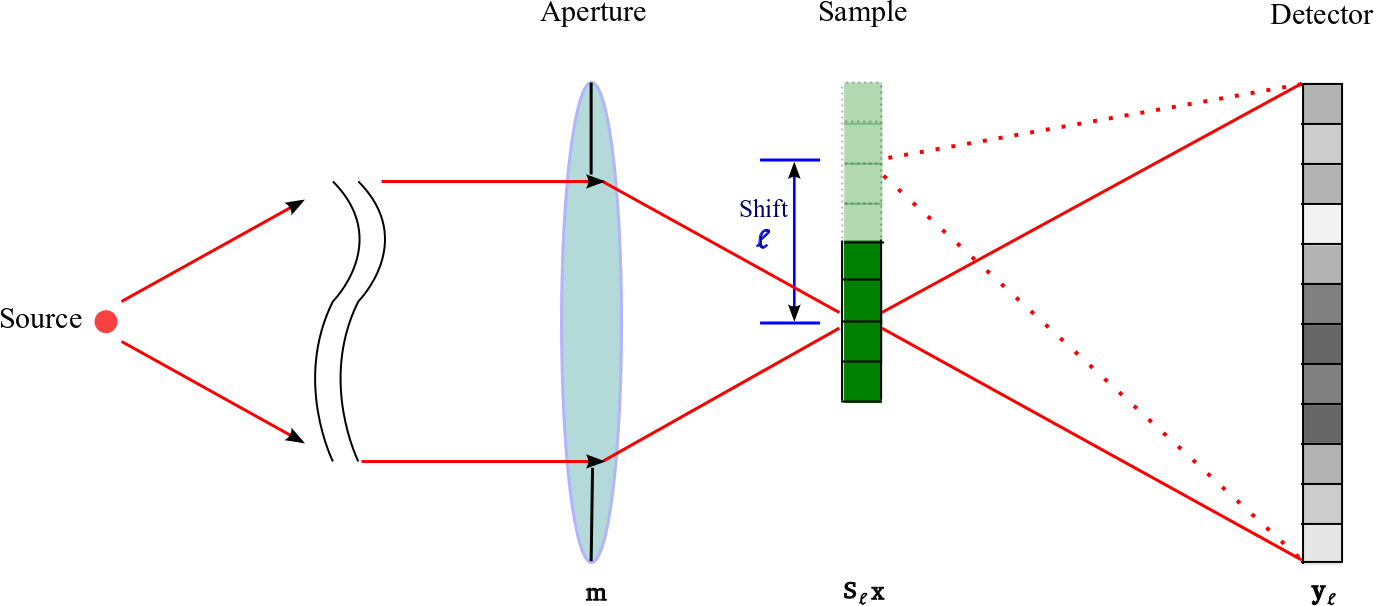
\includegraphics[scale=0.25]{pics/ptych1D}
    \caption{Illustration of one-dimensional ptychographic imaging {\small 
        (Adapted from ``Fly-scan ptychography'', Huang et al., 
        Scientific Reports 5 (9074), 2015.)} }
    \label{fig:ptychography_setup}
\end{figure}

In ptychographic imaging (see Fig.
\ref{fig:ptychography_setup}), small regions of a specimen are
illuminated one at a time and an intensity\footnote{By intensity,
we mean magnitude squared.} detector captures each of the
resulting  diffraction patterns. Thus each of the ptychographic
measurements is a local measurement, which under certain
assumptions (e.g., appropriate wavelength of incident radiation,
far-field Fraunhofer approximation), can be modeled as
\cite{Goodman2005IntroFourierOptics,Dierolf2008Ptych}%\RSnote{We need some citations here to justify this model}
%
\begin{equation}
    y(t, \omega) = \left \vert \mathcal F [ \widetilde h \cdot S_t f ] (\omega) 
       \right \vert^2 + \eta(t, \omega) .\label{eq:ptych}
\end{equation} 
%we acquire a sequence of possibly noisy, {\em local} (as
%opposed to {\em global}) snapshots of the magnitude of the underlying specimen. %The need
%to minimize the number of measurements acquired and inevitable
%measurement errors in the imaging process only accentuate the complexity
%of this phase retrieval problem.
%
%
%To set the stage for the discussion in this paper, consider the
%one-dimensional ptychographic imaging setup in Fig.~
%\ref{fig:ptychography_setup}, w
%Specifically, in the one-dimensional ptychography setting we focus on, . Under certain conditions (appropriate wavelength of
%incident radiation, far-field Fresnel approximation), it is possible to
%show \cite{?} that the acquired magnitude measurements of the form 
%%
%\begin{equation*}
%    y_\ell = \left \vert \mathcal F [ \widetilde m \circ S_\ell x ]
%       \right \vert^2,
%\end{equation*}
%%
Here, $\mathcal F$ denotes the Fourier transform, $f : [0, 1] \to \C$ represents
the unknown test specimen, $S_t$ is the shift operator defined
via $$(S_t f)(s) := f(s + t),$$ and $\widetilde h : [0, 1] \to \C$ is the so-called
illumination function %\RSnote{Aditya, is this standard terminology?} 
\cite{arXiv:1105.5628_MarchesiniEtAl}
of the imaging system. %Note that squaring the magnitude of the Fourier transform above means that $y_\ell$ is a
%phaseless diffraction measurement corresponding to a specific
%shift (by $\ell$) of the test specimen.  
To account for the local nature of the measurements in
\eqref{eq:ptych}, we assume that $\text{supp}(\widetilde h)
\subset \text{supp} (f)$.

As the phase retrieval problem is inherently non-linear and requires sophisticated computer algorithms to solve, consider the discrete version of \eqref{eq:ptych}, with $\widetilde{\m}, \x_0 \in \C^d$ discretizing $\widetilde{h}$ and $f$.  Thus \eqref{eq:ptych}, in the absence of noise, becomes 
%
\begin{equation}
    (\y_\ell)_j = \left \vert \sum_{n=1}^d \widetilde m_n \, (x_0)_{n+\ell} \,
      \mathbbm e^{-\frac{2\pi \mathbbm i (j-1) (n-1)}d} 
      \right \vert^2, \quad (j,\ell) \in [d] \times  
      [d]_0, 
  \label{eq:1d_ptycho}
\end{equation}
%
where indexing is
considered modulo-$d$, so $(\y_\ell)_j$
is a diffraction measurement corresponding to the $j^{th}$ Fourier mode
of a circular $\ell$-shift of the specimen. We use circular shifts for convenience and we remark that this is appropriate as one can zero-pad $\x_0$ and $\widetilde{\m}$  in \eqref{eq:1d_ptycho} and obtain the same $(\y_\ell)_j$ as one would with non-circular shifts. In practice, one may not need to use all the shifts $\ell \in [d]_0$ as a subset may suffice.  Defining $\m_j \in \C^d$ by \begin{equation} (\m_j)_n = \overline{\widetilde m_n} \, \mathbbm e^{\frac{2\pi \mathbbm i (j-1) (n-1)}d} \label{eq:ptychm} \end{equation} and rearranging \eqref{eq:1d_ptycho}, we obtain
\begin{align}
    (\y_\ell)_j &= \left \vert \sum_{n=1}^d (x_0)_{n+\ell} \, \overline{(\m_j)_n} \right \vert^2 \label{eq:loco_measurements} %\\ 
        %&
        = \left \vert \sum_{n=1}^\delta (x_0)_{n+\ell} \, \overline{(\m_j)_n} \right \vert^2 \\
        &= \lvert \langle S_\ell \x_0, \m_j \rangle \rvert^2 \notag %\\
       % &
       = \langle S_\ell \x_0 \x_0^* S_\ell^*, \m_j \m_j^* \rangle \notag\\
        &= \langle T_\delta(\x_0 \x_0^*), S_\ell^* \m_j \m_j^* S_\ell \rangle, \quad (j, \ell) \in [d] \times [d]_0 \notag
\end{align}
%
where the second and last equalities follow from the fact that $\widetilde \m$ (and hence each $\m_j$) is locally supported.  %% \RSnote{here be dragons: We have $d$ masks all generated from the same $\tilde{m}$ and then we would have $2\delta-1$ versions of them? Doesn't quite match up with our model later, so we need to address this somehow.}
We note that \eqref{eq:loco_measurements}
defines a correlation with local masks or window functions
$\m_j$.  More importantly, \eqref{eq:loco_measurements} shows that ptychography (with $\ell$ ranging over any subset of $[d]_0$) represents a case of the general system seen in \eqref{eq:lifted_system}.

\subsection{Connections to Masked Fourier Measurements}
%\RSnote{This should also be shortened and moved either to the intro under "Connections to Windowed-Fourier Measurements", or to the end...}
\label{sec:STFT}
%
%%
%
Often, in imaging applications involving phase retrieval, a mask is placed either between the illumination source and the sample or between the sample and the sensor. Here, we will see that the mathematical setup that we consider is applicable in this scenario, albeit when the masks are band-limited.  As before, let $\x_0, \m \in \mathbbm C^d$ denote the unknown signal of
interest, and a known mask (or window), respectively. Moreover, for a vector $\x_0 \in \C^d$ we denote its discrete Fourier transform $\widehat{\x_0} \in \mathbbm{C}^d$ by $$(\widehat{x_0})_k :=\sum_{n=1}^d (x_0)_n e^{-2\pi \mathbbm{i} (n-1)(k-1)/d}.$$  Here, we consider squared magnitude \emph{windowed Fourier
transform} measurements of the form 
%
\begin{equation}
  ({\y_\ell})_k = \left \vert \sum_{n=1}^d (x_0)_n \, m_{n-\ell} \,
      \mathbbm e^{-\frac{2\pi \mathbbm i (k-1) (n-1)}d} 
      \right \vert^2, ~ k \in [d],
      ~ \ell \in \{\ell_1, \dots, \ell_L\} \subset 
        [d]_0.
  \label{eq:STFT_measurements}
\end{equation}
%
As before, $\ell$ denotes a shift or translation of the mask/window, so
 $({\y_\ell})_k$ corresponds to the (squared magnitude of) the
$k^{th}$ Fourier mode associated with an
$\ell$-shift\footnote{As above, all indexing and shifts are considered
modulo-$d$.} of the mask $\m$. Defining the modulation operator, $W_k: \C^d \mapsto \C^d$,  by its action $(W_k \x_0)_n = e^{2\pi \mathbbm i (k-1)(n-1)/d}~(x_0)_n$ and applying elementary Fourier transform properties\footnote{$\widehat{S_\ell \x_0}=W_{\ell+1}\widehat{\x_0}$, $\widehat{W_k \x_0}=S_{-k+1}\widehat{\x_0}$, and $W_k S_\ell \x_0 = e^{-2\pi \mathbbm i (k-1)\ell/d} S_\ell W_k \x_0$.}
 one has
%
\begin{align}
    (\y_\ell)_k &=  \lvert \langle  \x_0, S_{-\ell}(e^{2\pi \mathbbm i (k-1)\ell/d}W_k\overline{\m} )\rangle \rvert^2 \notag \\
       & =  \lvert \langle  \x_0, S_{-\ell}(W_k \overline{\m} )\rangle \rvert^2 \notag 
       =  \lvert \langle  \widehat{\x_0}, \widehat{S_{-\ell}(W_{k} \overline{\m} )}\rangle \rvert^2 \notag \\
       & = \lvert \langle  \widehat{\x_0}, W_{-\ell+1}(S_{-k+1}\widehat{\overline{\m}} )\rangle \rvert^2 \notag \\ 
       &=\lvert \langle  \widehat{\x_0}, S_{-k+1}(W_{-\ell+1}\widehat{\overline{\m}} )\rangle \rvert^2.
       \end{align}

Defining $\widehat{\m}_\ell := W_{-\ell+1}\widehat{\overline{\m}}$ and assuming that $\supp(\widehat{\overline{\m}})\subset [\delta]$ (e.g., assuming that $\m$ is real-valued and band-limited), we now have that
\begin{align}%        \notag \\ 
%
    (\y_\ell)_{k}   &= \langle \widehat\x_0 \widehat\x_0^*, S_{-k+1} \widehat{\m}_\ell \widehat{\m}_\ell^* S_{-k+1}^*\rangle \notag\\
   &= \langle T_\delta(\widehat\x_0 \widehat\x_0^*), S_{-k+1} \widehat{\m}_\ell \widehat{\m}_\ell^* S_{-k+1}^*\rangle, \notag
%        &= \langle T_\delta(\x_0 \x_0^*), S_\ell^* \m_j \m_j^* S_\ell \rangle, \quad (j, \ell) \in [d] \times [d]_0 \notag
\end{align}
which again represents a case of the general system seen in \eqref{eq:lifted_system}. Moreover, our results all hold for this setting, albeit with the Fourier transforms of signals and conjugated masks.

%--------------------------------------------------
% Literature Survey 
%--------------------------------------------------
\subsection{Related Work}
\label{sec:lit}

%% --Alternating projection techniques \cite{gerchberg1972practical,fienup1978reconstruction} work well in practice and have been popular for decades, but are notoriously difficult to analyze.  These iterative methods work by improving an initial guess until they stagnate.  Recently Marchesini et al. proved that alternating projection schemes using generic measurements are guaranteed to converge to the correct solution {\em if provided with a sufficiently accurate initial guess}, and algorithms for ptychography were explored in particular \cite{marchesini2015alternating}.  However, no global recovery guarantees currently exist for alternating projection techniques utilizing local measurements (i.e., finding a sufficiently accurate initial guess is not generally easy).\\

%-- probabilistic recovery guarantees have been proven for many methods when provided with global gaussian measurements, including: methods based on convex optimization techniques \cite{candes2012phaselift,candes2014solving}, methods based on (stochastic) gradient decent strategies \cite{candes2015phase}, methods based on graph-theoretic and frame-based approaches  \cite{alexeev2014phase}, and alternating minimization methods variants (e.g., with resampling) \cite{netrapalli2013phase}. \\

The first approach to the phase retrieval problem was proposed in the 1970's in \cite{gerchberg1972practical} by Gerchberg and Saxton, where the measurement data corresponded to knowing the magnitude of both the image $\x_0$ and its Fourier transform.  This result was famously expanded upon by Fienup \cite{fienup1978reconstruction} later that decade, one significant improvement being that only the magnitude of the Fourier transform of $\x_0$ must be known in the case of a signal $\x_0$ belonging to some fixed convex set $\mathcal{C}$ (typically, $\mathcal{C}$ is the set of non-negative, real-valued signals restricted to a known domain).  Though these techniques work well in practice and have been popular for decades, they are notoriously difficult to analyze (see, e.g., \cite{takajo1997numerical,takajo1998study,takajo1999further,bauschke2002phase,bauschke2003hybrid,elser2003phase}).  These are  iterative methods that work by improving an initial guess until they stagnate.  Recently Marchesini et al.~proved that alternating projection schemes using generic measurements are guaranteed to converge to the correct solution {\em if provided with a sufficiently accurate initial guess} and algorithms for ptychography were explored in particular \cite{marchesini2015alternating}.  However, no global recovery guarantees currently exist for alternating projection techniques using local measurements (i.e., finding a sufficiently accurate initial guess is not generally easy).

Other authors have taken to proving probabilistic recovery guarantees when provided with globally supported Gaussian measurements.  Methods for which such results exist vary in their approach, and include convex relaxations \cite{candes2014solving,candes2012phaselift}, gradient descent strategies \cite{candes2015phase}, graph-theoretic  \cite{alexeev2014phase} and frame-based approaches \cite{balan2009painless, bodmann2013stable}, and variants on the alternating minimization (e.g., with resampling) \cite{netrapalli2013phase}.

Several recovery algorithms achieve theoretical recovery guarantees while using at most $D = \mathcal{O}(d \log^4 d)$ masked Fourier coded diffraction pattern measurements, including both {\em PhaseLift} \cite{Candes2014WF,gross2015improved}, and {\em Wirtinger Flow} \cite{candes2015phase}.  However, these measurements are both randomized (which is crucial to the probabilistic recovery guarantees developed for both PhaseLift and Wirtinger Flow -- deterministic recovery guarantees do not exist for either method in the noisy setting), and provide global information about $\x_0$ from each measurement (i.e., the measurements are not locally supported).

Among the first treatments of local measurements are \cite{eldar2014sparse,BendoryE16} and \cite{jaganathan2015stft}, in which it is shown that STFT measurements with specific properties can allow (sparse) phase retrieval in the noiseless setting, and several recovery methods are proposed.  Similarly, the phase retrieval approach from \cite{alexeev2014phase} was extended to STFT measurements in \cite{salanevich2015polarization} in order to produce recovery guarantees in the noiseless setting.  More recently, randomized robustness guarantees were developed for time-frequency measurements in \cite{pfander2016robust}.  However, no {\it deterministic} robust recovery guarantees have been proven in the noisy setting for any of these approaches.  Furthermore, none of the algorithms developed in these papers are empirically demonstrated to be competitive numerically with standard alternating projection techniques for large signals when utilizing windowed Fourier and/or correlation-based measurements.  In \cite{IVW2015_FastPhase}, the authors propose the measurement scheme developed in the current paper and prove the first deterministic robustness results for a different greedy recovery algorithm.

%% -- early mathy phase retrieval papers \cite{balan2006signal,balan2009painless}.\\

%% -- 
%%-- About convergence of ER \cite{takajo1997numerical}\\
%%-- About convergence of HIO \cite{takajo1998study}\\
%%-- More on HIO convergence \cite{takajo1999further}\\
%%-- A reformulation of ER and HIO as convex optimization methods, \cite{bauschke2002phase}\\
%%-- Another optimization-based method that is "competitive with HIO", no theory \cite{bauschke2003hybrid} \\
%%-- The difference map approach -- another HIO-like optimization-based approach \cite{elser2003phase}

%-- Local measurements:  In \cite{eldar2014sparse,jaganathan2015stft} it is shown that STFT measurements with specific properties can allow (sparse) phase retrieval in the noiseless setting, and several recovery methods are proposed.  Similarly, the phase retrieval approach from \cite{alexeev2014phase} is extended to STFT measurements in \cite{salanevich2015polarization} in order to produce recovery guarantees in the noiseless setting. However, no recovery guarantees are proven in the noisy setting for any of these approaches.  Aditya and my paper \cite{IVW2015_FastPhase}...\\


%-------------------------------------------------------------------------------------------

\subsection{Organization}  Section \ref{sec:MeasMatrix} discusses two collections of local correlation masks $\m_j$, one of which is novel and the other of which was originally studied in \cite{IVW2015_FastPhase}.  Most importantly, Section \ref{sec:MeasMatrix} shows that the recovery of $T_\delta(\x_0\x_0^*)$ from measurements associated with the proposed masks can be done stably in the presence of measurement noise. %and then briefly introduces the new lifting-based phase retrieval approach for local measurements considered herein.  
%The new recovery algorithm for local
%correlation measurements is then discussed in detail in Section~\ref{sec:TheAlg}, and it is shown in Section~\ref{sec:STFT} that the same approach can also be 
%used to solve the problem of phase retrieval from Short Time Fourier Transform (STFT) magnitude measurements. 
Moreover, since in the noisy regime, the leading eigenvector $\widetilde{\x}$ of $\widetilde{X}$ (associated with line 3 of Algorithm \ref{alg:phaseRetrieval1}) will no longer correspond exactly to the true phases $\widetilde{\x}_0$, we are interested in a perturbation theory for the eigenvectors of $\widetilde{X}_0$.  Intuitively, $\widetilde{\x}$ will be most accurate when the eigenvalue of $\widetilde X_0$ associated with $\widetilde{\x}_0$ is well separated from the rest of the eigenvalues and so, accordingly, Section~\ref{sec:Spectrum} studies the spectrum of $\widetilde X_0$.  Indeed, this eigenvalue is rigorously shown to control the stability of the top eigenvector of $\widetilde{X}_0$ with respect to noise, and Section~\ref{sec:Perturb} develops perturbation results concerning their top eigenvectors by adapting the spectral graph techniques used in \cite{alexeev2014phase}.  Recovery guarantees for the proposed phase retrieval method are then compiled in Section~\ref{sec:RecovGuarantee}.  Numerical results demonstrating the accuracy, efficiency, and robustness of the proposed methods are finally provided in Section \ref{sec:NumEval}\footnote{MATLAB code to run the BlockPR algorithm is available online at \cite{bitbucket_BlockPR}.}, while Section \ref{sec:conclusion} contains some concluding remarks and avenues for further research.  In Appendix~\ref{sec:AltPerturbBounds}, we provide an alternate, weaker but easier to derive eigenvector perturbation result analogous to the one in Section \ref{sec:Perturb} which may be of independent interest.


\section{Well-conditioned measurement maps}
\label{sec:MeasMatrix}
Here, we present two example constructions for which the linear operator $\mathcal{A}|_{T_\delta(\C^{d\times d})}$ used in Step 1 of Algorithm \ref{alg:phaseRetrieval1} is well conditioned. Such constructions are crucial for the stability of the method to additive noise. 

\subsection*{Example 1:} 
In \cite{IVW2015_FastPhase}, a construction was proposed for the masks $\m_\ell$ in \eqref{eq:shift_model} that guarantees the stable invertibility of $\mathcal{A}$.  This construction comprises windowed Fourier measurements with parameters $\delta \in \mathbbm{Z}^+$ and $a \in [4, \infty)$ corresponding to the $2\delta-1$ masks $\m_j\in\C^d$, $j=1,...,2\delta-1$ with entries given by
%
\begin{equation}
(\m_j)_{n} = \left\{ \begin{array}{ll}
    \frac{\ee^{-n/a}}{\sqrt[4]{2\delta -1}} \cdot
    \ee^{\frac{2 \pi \ii \cdot (n - 1) \cdot (j -1)}
    {2\delta - 1}} & \textrm{if}~n \leq \delta \\ 
    0 & \textrm{if}~n >  \delta\end{array} \right. .
    \label{eq:MeasDef}
\end{equation}
%
Here, measurements using all shifts $\ell = 1,..., d$ of each mask are taken.  In the notation of \eqref{eq:lifted_system}, this corresponds to  $K = 2\delta - 1$ and $P = [d]_0$, which yields $D = (2\delta - 1)d$ total measurements.  By considering the basis $\{E_{ij}\}$ for $T_\delta(\C^{d \times d})$ given by %\[(E_{ij})_{st} = \delta_{(i, j)}(s, t), \quad \text{for} \ |i - j| \mod d < \delta,\] where $\delta_{(i,j)}$ denotes the Dirac delta with 
\begin{align}\nonumber
E_{i,j}(s,t) =\left\{\begin{array}{l} 1, \quad (i,j)=(s,t)\\ 0, \quad \text{otherwise}\end{array}\right.
\end{align}
it was shown in \cite{IVW2015_FastPhase} that this system is both well conditioned and rapidly invertible.  In particular, if $M'$ is the matrix representing the measurement mapping $\mathcal{A} : T_{\delta}(\C^{d \times d}) \to T_{\delta}(\C^{d \times d})$ with respect to the basis $\{E_{ij}\}$, the following estimates of the condition number and cost of inversion hold.

\begin{thm}[\cite{IVW2015_FastPhase}]
Consider measurements of the form \eqref{eq:MeasDef} with $a:= \max \left\{ 4,~\frac{\delta - 1}{2} \right\}$. 
Let $M' \in \C^{D \times D}$ be the matrix representing the measurement mapping $\mathcal{A} : T_{\delta}(\C^{d \times d}) \to T_{\delta}(\C^{d \times d})$ with respect to the basis $\{E_{ij}\}$.  Then, the condition number of $M'$ satisfies 



%Let $M' \in \mathbbm{C}^{D \times D}$ be the matrix representing the measurement mapping $\mathcal{A} : T_{\delta}(\C^{d \times d}) \to T_{\delta}(\C^{d \times d})$ with respect to the basis $\{E_{ij}\}$, and consider measurements of the form \eqref{eq:MeasDef} using parameters $a:= \max \left\{ 4,~\frac{\delta - 1}{2} \right\}$.  Then, the condition number of $M'$ satisfies 
%
$$\kappa \left( M' \right) ~<~ \max
\left\{ 144 \ee^2,~\frac{9 \ee^2}{4} \cdot (\delta -
1)^2 \right \},$$
%
and the smallest singular value of $M'$ satisfies
%
$$\sigma_{\rm min} \left( M' \right) > \frac{7}{20 a} \cdot \ee^{-(\delta + 1)/a} > \frac{C}{\delta}$$
%
for an absolute constant $C \in \R^+$.  Furthermore, $M'$ can be
inverted in $\mathcal{O} \left( \delta \cdot d \log d \right)$-time.
\label{thm:WellCondMeas}
\end{thm}

This theorem indicates that one can both efficiently and stably solve for $\x_0 \x_0^*$ using \eqref{eq:lifted_system} with the measurements given in \eqref{eq:MeasDef}.   This measurement scheme is also interesting because it corresponds to a ptychography system if we take the illumination function (i.e.~the physical mask) in \eqref{eq:1d_ptycho} to be $\widetilde{m}_n = \frac{\ee^{- n / a}}{\sqrt[4]{2 \delta - 1}}$ and assume that $d = k(2 \delta - 1)$ for some $k \in \N$; in practice, this may be achieved by zero-padding the specimen.  Then we may take the subset of the measurements \eqref{eq:ptychm} given by $j = (p -1)k + 1, \ p \in [2 \delta - 1]$ to obtain the masks specified in \eqref{eq:MeasDef}.  We also remark that in this setup, only one physical mask is required, as the index $j$ in \eqref{eq:MeasDef} denotes the different frequencies observed in the Fourier domain at the sensor array.


\subsection*{Example 2:} We provide a second deterministic construction that improves on the condition number of the previous collection of measurement vectors.  We merely set $\m_1 = e_1, \m_{2j} = e_1 + e_{j+1}$, and 
% m_2j needs to be + i e_j+1 (plus) to account for complex conj. in inner prod.
$\m_{2j + 1} = e_1 + i e_{j+1}$ for $j = 1, \ldots, \delta - 1$.  A simple induction shows that $\{S_\ell \m_j \m_j^* S_\ell^*\}_{\ell \in [d]_0, j \in [2k - 1]}$ is a basis for $T_k(\C^{d \times d})$, so if we take $\m_1, \ldots, \m_{2\delta - 1}$ for our masks we'll have a basis for $T_{\delta}(\C^{d \times d})$.  Indeed, if we let $$\mathcal{B} : T_k(\C^{d \times d}) \to \C^{\delta \times d}$$ be the measurement operator defined via 
%
$$\big(\mathcal{B}(X)\big)_{\ell, j} = \langle S_\ell \m_j \m_j^* S_\ell^*, X \rangle, \quad (\ell, j) \in [d]_0 \times [2k - 1]$$
we can immediately solve for the entries of $X \in T_k(\H^{d \times d})$ from $\mathcal{B}(X) =: B$ by observing that \[\begin{array}{rcl}
X_{i,i} & = & B_{i - 1,1} \\
X_{i, i + k} & = & \frac{1}{2}B_{i - 1, 2k} + \frac{i}{2}B_{i - 1, 2k + 1} - \frac{1 + i}{2} (B_{i - 1, 1} + B_{i + k - 1, 1}), \end{array}\] where we naturally take the indices of $B$ mod $d$.  This leads to an upper triangular system if we enumerate $X$ by its diagonals; namely we regard $T_\delta(\H^{d \times d})$ as a $d(2 \delta - 1)$ dimensional vector space over $\R$ and set, for $i \in  [d]$ 
%
\[\begin{array}{ll}
z_{kd + i} =  \left\{\begin{array}{r@{,\quad}l} \operatorname{Re}(X_{i, i + k}) & 0 \le k < \delta \\ \operatorname{Im}(X_{i, i + k - \delta + 1}) & \delta \le k < 2\delta - 1 \end{array}\right., \ \ 
y_{kd + i}  =  \left\{\begin{array}{r@{,\quad}l} \mathcal{B}(X)_{i, 1} & k = 0 \\ \mathcal{B}(X)_{i, 2k} & 1 \le k < \delta \\  \mathcal{B}(X)_{i, 2(k - \delta + 1) + 1} & \delta \le k < 2 \delta - 1 \end{array}\right.
\end{array}. \] Then with $S = S_1 \in \R^{d \times d}$ representing the circular shift operator as before, we have  %
%
%\[y = \begin{bmatrix} I & 0 & 0 & \cdots & 0 \\ -(I + S)/2 & I/2 & 0 & \cdots & 0 \\ \vdots & & \ddots & & \\ I + S^{\delta - 1} & 0 & \cdots & 0 & I \end{bmatrix} z =: Cz.\]  
\[y = \begin{bmatrix} I_d & 0 & 0 \\ D & 2 I_{d(\delta - 1)} & 0 \\ D & 0 & 2 I_{d(\delta - 1)} \end{bmatrix}z =: Cz, \ \text{where} \ D = \begin{bmatrix} I_d + S \\ I_d + S^2 \\ \vdots \\ I_d + S^{\delta - 1} \end{bmatrix}.\]  Since the matrix $C$ is upper triangular, its inverse is immediate: \[C^{-1} = \begin{bmatrix} I_d & 0 & 0 \\ -D / 2 & I_{d(\delta-1)} / 2 & 0 \\ -D / 2 & 0 & I_{d(\delta-1)} / 2 \end{bmatrix}.\]  To ascertain the condition number of $\mathcal{B}$% of solving for $X$ from $\mathcal{B}(X)$
, then, all we need is the extremal singular values of $C$.  We bound the top singular value by considering 
\[\begin{array}{rcl} \sigma_{\max}(C) = \max\limits_{||w||^2 + ||v||^2 = 1} \left\lVert C\begin{bmatrix} w \\ v \end{bmatrix} \right\rVert  & = & \left\lVert \begin{bmatrix} w \\ D w \\ D w \end{bmatrix} + 2\begin{bmatrix} 0 \\ v \end{bmatrix} \right\rVert \\
& \le & \sqrt{||w||^2 + 2 ||w + Sw||^2 + \cdots + 2 ||w + S^{\delta - 1} w||^2} + ||2 v|| \\
& \le & \sqrt{8 (\delta - 1) + 1}||w|| + 2 ||v|| \le \sqrt{8(\delta - 1) + 5} \le 2\sqrt{2 \delta},  \end{array}\]  where in the last line we have used $||w||^2 + ||v||^2 = 1$.  By a nearly identical argument, we find \[\dfrac{1}{\sigma_{\min}(C)} = \sigma_{\max}(C^{-1}) \le \sqrt{2 \delta}\] so that the condition number is bounded by $\kappa(C) \le 4\delta$.
%\RSnote{Brian, check this: I think the constants are off.}\BPnote{Checked and changed!}


%%%%%%%%%%%%%%%%%%%%%%%%%%%%%%%%%%%%%%%%%%%%%%%%%%%%%%%
%% \section{Fast Phase Retrieval from Local Correlation Measurements}
%% \label{sec:fastloco}
%% %
%%
%
We now summarize a new %recently introduced \cite{IVW2015_FastPhase} 
fast (essentially linear-time) approach for recovering $\x_0$ from local
correlation measurements of the form (\ref{eq:loco_measurements}). 
More explicitly, we will consider the problem of recovering $\x_0 \in \mathbbm C^d$ from noisy
magnitude measurements $\y \in \mathbbm{R}^D$ of the form 
%
\begin{equation}
    \y = \left | M \x_0 \right |^2 + \n, 
    \label{equ:MeasModel}
\end{equation}
%
with $D \geq d$.  Here $M \in \mathbbm{C}^{D \times d}$ is our
measurement matrix, $| \cdot |^2: \mathbbm{C}^D \rightarrow
\mathbbm{R}^D$ computes the  componentwise squared magnitude of each
vector entry, and $\n \in \mathbbm{R}^D$ represents arbitrary
measurement noise.  Note that we will always consider the indices of vectors in
$\mathbbm{C}^d$ to be $\mod d$ and between $1$ and $d$; more
specifically, for any $\z \in \mathbbm{C}^d$, we always mean to indicate the entry 
$z_{(j-1) \mod d \ + 1}$ whenever we write $z_j$.


\subsection{A Banded Lifting Scheme}
\label{sec:LiftToBandedMatrix}

Solving for $\z$ via \eqref{equ:LinProb} in the noiseless setting yields a portion of the rank one matrix ${\bf x}_0 {\bf x}_0^*\in \mathbbm{C}^{d \times d}$.  More specifically, only the diagonal entries are recovered as part of the banded matrix
\begin{equation}
(\X_0)_{j,k} =  \left\{ \begin{array}{ll} ({\bf x}_0 {\bf x}_0^*)_{j,k} & \textrm{if}~| j - k ~{\rm mod}~d | < \delta \\ 0 & \textrm{otherwise} \end{array} \right..
\label{equ:PhaseMatrix}
\end{equation}
Normalizing each entry of $\X_0 \in \mathbbm{C}^{d \times d}$ one obtains the Hermitian matrix $\tilde{\X}_0 \in \mathbbm{C}^{d \times d}$ with entries
\begin{equation}
(\tilde{\X}_0)_{j,k} =  \left\{ \begin{array}{ll} \mathbbm{e}^{\mathbbm{i}(\phi_j - \phi_k)} & \textrm{if}~| j - k ~{\rm mod}~d | < \delta \\ 0 & \textrm{otherwise} \end{array} \right.,
\label{equ:MatrixofPhases}
\end{equation}
where $(x_0)_j = r_j \mathbbm{e}^{\mathbbm{i} \phi_j}$ for $j \in [d]$.  Our objective is now to use $\X_0 \in \mathbbm{C}^{d \times d}$ to recover $\phi_1, \dots, \phi_d \in [0, 2 \pi]$, the phases of the entries of ${\bf x}_0$.  That is, we want to recover the vector ${\bf \tilde{x}}_0 \in \mathbbm{C}^d$ with 
\begin{equation}
(\tilde{x}_0)_j := \mathbbm{e}^{\mathbbm{i}\phi_j} ~=~ \left\{\begin{array}{ll} (x_0)_j / |(x_0)_j| & \textrm{if}~|(x_0)_j| \neq 0\\ 1 & \textrm{else} \end{array} \right.
\label{Def:VecofPhases}
\end{equation} 
using $\tilde{\X}_0$.  The following theorem, proven in \cite{IV_SPIE}, demonstrates that this is possible in the noiseless setting by simply computing the top eigenvector of $\tilde{\X}_0$.  

\begin{thm}
The largest magnitude eigenvalue of $\tilde{\X}_0$ is $\nu_1 = 2 \delta -1$, and $\tilde{\x}_0$ is the only eigenvector of $\tilde{\X}_0$ with eigenvalue $\nu_1$.  Furthermore, $c \sqrt{\sum^d_{j=2} \nu^2_j} \leq \nu_1$ whenever $\delta \geq \frac{1+(d+1) c^2}{2(1+c^2)}$ for any chosen $c \in \mathbbm{R}^+$.
\label{thm:Noiseless_Spectrum}
\end{thm}

As demonstrated below, computing the leading eigenvector of $\tilde{\X}_0$ also turns out to be both highly robust to noise numerically, as well as provably robust theoretically.  In order to see this, explicit formulas are developed for the entire spectrum of any such $\tilde{\X}_0$ matrix below, in \S \ref{sec:Spectrum}.  Besides improving on Theorem~\ref{thm:Noiseless_Spectrum}, these formulas, when combined with matrix perturbation results, allow us to bound the effect of noise on the leading eigenvector of $\tilde{\X}_0$ in \S \ref{sec:Perturb}.  These bounds are then carefully combined with properties of the proposed measurements (e.g., Theorem~\ref{thm:WellCondMeas}) in order to develop theoretical robustness guarantees for the overall phase retrieval approach in \S \ref{sec:RecovGuarantee}.  The end result is a new phase retrieval method for measurements of the type discussed above (recall \S \ref{sec:MeasMatrix}) which is significantly more robust to noise than similarly fast methods for locally supported measurements.  We are now ready to begin by explicitly specifying our recovery algorithm in full detail.



%%%%%%%%%%%%%%%%%%%%%%%%%%%%%%%%%%%%%%%%%%%%%%%%%%%%%%%
%\section{An Improved Recovery Algorithm for Locally Supported Measurements}
%\label{sec:TheAlg}
%
In this section we will formalize and discuss the phase retrieval method outlined in Section~\ref{sec:intro}.  It is also summarized below in Algorithm~\ref{alg:phaseRetrieval}.  In short, the method can be subdivided into three simple stages:  During the first stage a linear system corresponding to the utilized measurements is inverted in order to approximately recover the diagonal entries of the rank-one matrix $\x_0 \x^*_0$ (see line 1 of Algorithm~\ref{alg:phaseRetrieval}).  Due to its special structure, the associated measurement matrix $M'$ from the construction of \eqref{eq:MeasDef} can be inverted in just $\mathcal{O} \left( \delta \cdot d \log d \right)$-time by performing $\mathcal{O(\delta)}$ fast Fourier transforms (see Theorem~\ref{thm:WellCondMeas}, and \cite{IVW2015_FastPhase} for additional details).  

During its second stage, the algorithm reorganizes its estimates of the diagonal entries of $\x_0 \x^*_0$ into a Hermitian, banded, and entry-wise normalized matrix $\tilde{\X}$ (see lines 2-4).  The leading eigenvector of this $\tilde{\X}$, which provides estimates of the phases of each entry in $\x_0$, is then computed (see line 5).  Finally, during its third stage, the algorithm approximates the magnitudes of each entry of $\x_0$, and then uses them to construct its final estimate of $\x_0$ (see line 6).

\begin{algorithm}
\renewcommand{\algorithmicrequire}{\textbf{Input:}}
\renewcommand{\algorithmicensure}{\textbf{Output:}}
\caption{Fast Phase Retrieval from Local Correlation Measurements}
\label{alg:phaseRetrieval}
\begin{algorithmic}[1]
    \REQUIRE Measurements $\y = |  M \x_0 |^2 + \n \in \mathbbm{R}^D$ as per \eqref{equ:shift_model}
    \ENSURE ${\bf x} \in \mathbbm{C}^d$ with ${\bf x} \approx \mathbbm{e}^{-\mathbbm{i} \theta} {\bf x}_0$ for some $\theta \in [0, 2 \pi]$ 
    \STATE Compute ${\bf z}' = (M')^{-1} P {\bf y}$ (see \eqref{equ:LinProb}) %--[??? use ${\bf z}' = W (M')^{-1} P {\bf y}$ instead -- see \eqref{def:Wdef}) ?]
    \STATE Form a banded matrix $\Y \in \mathbbm{C}^{d \times d}$ from $\z'$ as per \eqref{equ:PhaseMatrix} in \S\ref{sec:LiftToBandedMatrix}
    \STATE Ensure Hermitianity by setting $\X = (\Y + \Y^*) / 2$
    \STATE Form the Hermitian banded matrix of phases, $\tilde{\X} \in \mathbbm{C}^{d \times d}$, by normalizing the entires of $\X$ %(replacing any zero entries in the band with $1$'s)
    \STATE Compute the top eigenvector of $\tilde{\X}$, $\u \in \mathbbm{C}^d$ and a normalized version $\tilde{\x}$ with $\tilde{x}_i = u_i / |u_i|$
    \STATE Set $x_j = \sqrt{X_{j,j}} \cdot \tilde{x}_j$ for all $j \in [d]$ to form $\x \in \mathbbm{C}^d$
    %\STATE Set $\x = W^* \tilde{\x}$ 
    \end{algorithmic}
\end{algorithm}

\BPnote{The algorithm seems to be ``first construction'' specific.  Should we change step 1 and 2 to reflect that we're inverting an arbitrary linear system on the lifted space?}. \RSnote{I think this entire subsection goes, and the speed calculation can be put into example 1 of the "well-conditioned measurement maps" section.}

In the low-noise regime (i.e, $\n \approx {\bf 0}$), computing the top eigenvector of $\tilde{\X} \approx \tilde{\X_0}$ to $\epsilon$-precision using the power method in line 5 will require a number of iterations determined by $\frac{\nu_2}{\nu_1}$, where $\nu_1$ and $\nu_2$ are the largest and second largest eigenvalues of $\tilde{\X_0}$, respectively.  Referring to Lemma~\ref{lem:spectrum} and the proof of Lemma~\ref{lem:EigGap} in \S \ref{sec:Spectrum} one can see that
\begin{align*}
\frac{\nu_2}{\nu_1} &= \frac{1 + 2 \sum_{k = 1}^{\delta - 1}\cos\left(\bigfrac{2\pi k}{d}\right)}{2 \delta - 1} \leq \frac{1 + 2 (\delta - 1) \cos (\pi \delta / d)}{2 \delta - 1} \leq  \frac{1 + 2 (\delta - 1) \left(1 - \frac{1}{2} \left(\frac{\pi \delta}{d} \right)^2 + \frac{1}{12} \left(\frac{\pi \delta}{d} \right)^4 \right)}{2 \delta - 1}\\
& \leq 1 - \left(\frac{1}{2} \left(\frac{\pi \delta}{d} \right)^2 - \frac{1}{12} \left(\frac{\pi \delta}{d} \right)^4 \right)\frac{2}{3}
\end{align*}
for all $d \geq \delta \geq 2$.  This implies that using
\begin{align*}
\frac{\ln(\epsilon/d)}{\ln \left(1 - \left(\frac{1}{3} \left(\frac{\pi \delta}{d} \right)^2 - \frac{1}{18} \left(\frac{\pi \delta}{d} \right)^4 \right) \right)} &= \frac{\ln(d/ \epsilon)}{ \sum^{\infty}_{n=1} \frac{1}{n} \left(\frac{1}{3} \left(\frac{\pi \delta}{d} \right)^2 - \frac{1}{18} \left(\frac{\pi \delta}{d} \right)^4 \right)^n}\\ 
&\leq \frac{\ln(d/ \epsilon)}{ \frac{1}{3} \left(\frac{\pi \delta}{d} \right)^2 - \frac{1}{18} \left(\frac{\pi \delta}{d} \right)^4 } = \mathcal{O}\left( \frac{d^2 \ln (d/\epsilon)}{\delta^2} \right)
\end{align*}
power method iterations should generally suffice in order to provide an $\mathcal{O}(\epsilon)$-accurate approximation to the leading eigenvector of $\tilde{\X}$ in line 5 of Algorithm~\ref{alg:phaseRetrieval}.
If computed by repeatedly squaring/rescaling $\tilde{\X}$ $\mathcal{O} \left(\log (d/\delta) \cdot \log \log (d/\epsilon)  \right)$-times before applying the result to a randomly chosen initial vector, one can expect to achieve an $\mathcal{O}(\epsilon)$-accurate answer in worst case $\mathcal{O}(d^2 \log (d/\delta) \cdot \log \log (1/\epsilon) )$-time.  Numerically, however, it appears as if $\mathcal{O}(\log^c d)$ power iterations\footnote{Herein, $c$ always represents an arbitrary positive constant.} usually suffice when the initial vector is deterministically chosen to be, e.g., $\mathbbm{1}$ (the vector of all ones).  Hence, the runtime of line 5 is typically $\mathcal{O}(\delta \cdot d \log^c d )$-time.  \RSnote{We need to rework this -- we believe it should have a $d^3$ somewhere in the worst case runtime, at least we couldn't beat it as we worked through this.  Specifically, if we have $\dfrac{d^2}{\delta^2} \ln(d / \epsilon)$ iterations, and each one costs $d \cdot \delta^2$ (from sparsity), you end up with $d^3 \log(1 / \epsilon)$.  Also, the repeated squaring costs $~d^3$ for each square (we lose bandedness), so we couldn't find a speedup there.  Are you using the structure to compute things in Fourier?  If so, please flesh it out.}

In practice, then, the total runtime complexity of Algorithm~\ref{alg:phaseRetrieval} is generally $\mathcal{O}(d \log^c d)$ whenever $\delta$ is allowed to scale at most poly-logarithmically in $d$.  See Section~\ref{sec:NumEval} for additional discussion, and the next section for more information concerning techniques for estimating the magnitudes of each entry in $\x_0$.

\subsection{An Improved Magnitude Estimation Method}\RSnote{Two options: we either remove this, as it would be the basis of another paper, or we keep it and move it to the end, under a section named "Extensions" or "Future work" or something like this.}

Looking at the matrix $\X$ formed on line 3 of Algorithm~\ref{alg:phaseRetrieval} one can see that
$$\X= \X_0 + N'$$
where $\X_0$ is the banded Hermitian matrix defined in \eqref{equ:PhaseMatrix}, and $N'$ contains arbitrary banded Hermitian noise.  As stated (and analyzed below) Algorithm~\ref{alg:phaseRetrieval} takes advantage of this structure in line 6 in order to estimate the magnitude of each entry of $\x_0$ based on the fact that 
$$\X_{j,j} = |(x_0)_{j}|^2 + N'_{j,j}$$
holds for all $j \in [d] := \{ 1, \dots, d\}$.  Though this magnitude estimate suffices for our theoretical treatment below, it can be improved on in practice by using slightly more general techniques.

Considering the component-wise magnitude of $X$, $|X| \in \mathbbm{R}^{d \times d}$, one can see that its entries are 
\begin{equation*}
|\X|_{j,k} =  \left\{ \begin{array}{ll} |({x}_0)_j| |({x}_0)_{k}| + N''_{j,k} & \textrm{if}~| j - k ~{\rm mod}~d | < \delta \\ 0 & \textrm{otherwise} \end{array} \right.,
\end{equation*}
where $N'' \in \mathbbm{R}^{d \times d}$ represents the changes in magnitude to the entries of $|\X_0|$ due to noise. %% For example, if $\delta = 2$ and $d = 4$ then
%% \[ |X| = \begin{bmatrix}
%%     & |(x_0)_1|^2 & &
%%     |(x_0)_1||(x_0)_2| & & 
%%     0 & &
%%     |(x_0)_1||(x_0)_4| & \\
%%     & 
%%     |(x_0)_2||(x_0)_1| & &
%%     |(x_0)_2|^2 & &
%%     |(x_0)_2||(x_0)_3| & &
%%     0 & \\
%%     & 0 & & 
%%     |(x_0)_3||(x_0)_2| & &
%%     |(x_0)_3|^2 & &
%%     |(x_0)_3||(x_0)_4| & & \\
%%     & |(x_0)_4||(x_0)_1| & &
%%     0 &  &
%%     |(x_0)_4||(x_0)_3| & &
%%     |(x_0)_4|^2 &
%% \end{bmatrix} + N''.    \]
%% Next, for any such matrix $|X|$, let $D_j \in \mathbbm{R}^{\delta \times \delta}$ denote its sub-matrix whose entries are given by 
%% $$(D_j)_{k,h} = |X|_{(j+k-1)~{\rm mod}~d,~(j+h-1)~{\rm mod}~d},$$
%% where $j \in [d]$.  Thus, in our example above with $\delta = 2$ and $d = 4$, we would have
%% \[ D_2 = \begin{bmatrix}
%%     |(x_0)_2|^2 & |(x_0)_2||(x_0)_3| \\
%%     |(x_0)_3||(x_0)_2| & |(x_0)_3|^2 
%% \end{bmatrix} + N_2'', ~{\rm and}~D_4 = \begin{bmatrix}
%%     |(x_0)_4|^2 & |(x_0)_4||(x_0)_1| \\
%%     |(x_0)_1||(x_0)_4|&  |(x_0)_1|^2 
%%     \end{bmatrix} + N''_4,
%% \]
%% where $N''_2, N''_4 \in \mathbbm{R}^{2 \times 2}$ are sub-matrices of the symmetric noise matrix $N''$.  It is important to note that these $D_j$ will always be rank-one matrices, plus symmetric noise.  As such, we may estimate the magnitudes $|(x_0)_j|, ~|(x_0)_{j+1}|,~ \dots,~ |(x_0)_{j+\delta-1}|$ by computing the leading eigenvector of $D_j$ for any desired $j \in [d]$.
We may then let $D_j \in \R^{\delta \times \delta}$ denote the submatrix of $|X|$ given by \[(D_j)_{k,h} = |X|_{(j+k-1)~{\rm mod}~d,~(j+h-1)~{\rm mod}~d},\] for all $j \in [d]$; similarly we let $N_j''$ denote the respective submatrices of $N''$.  With this notation, it is clear that \[D_j = |\x_0|^{(j)} (|\x_0|^{(j)})^* + N_j'',\] where $|\x_0|^{(j)}_k = |\x_0|_{k + j - 1}, k \in [\delta]$.  This immediately reveals that we can estimate the magnitudes of the entries of $\x$ by calculating the top eigenvectors of these submatrices!

Indeed, if we do so for all of $D_1, \dots, D_d \in \mathbbm{R}^{\delta \times \delta}$, we will produce $\delta$ estimates for each entry's magnitude.  A final estimate of each $|(x_0)_j|$ can then be computed by taking the average, median, etc. of the $\delta$ different estimates of $|(x_0)_j|$ provided by each of the leading eigenvectors of $D_{j-\delta+1}, \dots, D_j$.  Of course, one need neither use all $d$ possible $D_j$ matrices, nor make them have size $\delta \times \delta$.  More generally, to reduce computational complexity, one may instead use $d/s$ matrices, $\tilde{D}_{j'} \in \mathbbm{R}^{\gamma \times \gamma}$, of size $1 \leq \gamma \leq \delta$ and with shifts $s \leq \gamma$ (dividing $d$), having entries
$$(\tilde{D}_{j'})_{k,h} = |X|_{(sj'+k-1)~{\rm mod}~d,~(sj'+h-1)~{\rm mod}~d}.$$
Computing the leading eigenvectors of $\tilde{D}_{j'}$ for all $j' \in [d/s]$ will then produce (multiple) estimates of each $|(x_0)_j|$ which can then be averaged, etc., as desired in order produce our final magnitude estimates.  As we shall see below in \S \ref{sec:NumEval}, one can achieve better numerical robustness to noise using this technique than what can be achieved using the simpler magnitude estimation technique presented in line 6 of Algorithm~\ref{alg:phaseRetrieval}.  The theoretical analysis of this method is relegated to future work. \BPnote{Although I'm starting to think we can get something here rather quickly out of lemma 4}\RSnote{The numbering may have changed, are you sure you mean Lemma 4?}


We are now prepared to begin analyzing the performance of Algorithm~\ref{alg:phaseRetrieval} in detail.  We will begin this process by considering the spectral properties of any matrix $\tilde{\X}_0$ formed as in \eqref{equ:MatrixofPhases}.  This spectral information will ultimately help us to understand the robustness of line 5 in Algorithm~\ref{alg:phaseRetrieval} to noise.


%%%%%%%%%%%%%%%%%%%%%%%%%%%%%%%%%%%%%%%%%%%%%%%%%%%%%%%
\section{The Spectrum of $\tilde{\X}_0$}
\label{sec:Spectrum}
%Let $\delta \in \N$ be such that $\delta \le \lfloor \frac{d+1}{2} \rfloor$.  Theorem~\ref{thm:Noiseless_Spectrum} guarantees that $\widetilde{X}_0$ from \eqref{equ:MatrixofPhases} has $\widetilde{\x}_0$ as its (unique) top eigenvector with eigenvalue $\nu_1 = 2 \delta -1$.  This combined with the fact that $\| \widetilde{X}_0 \|_{\rm F} = \sqrt{d (2 \delta - 1)}$ and ${\rm Tr}(\widetilde{X}_0) = d$ suggests that line 5 of Algorithm~\ref{alg:phaseRetrieval} is likely to produce a reasonably accurate approximation to $\widetilde{\x}_0$ as long as $\| \n \|_2$ is sufficiently small and $\delta$ is sufficiently large.  Of course, more detailed knowledge regarding the spectral properties of $\widetilde{X}_0$ are required before such observations can be made precise.  In this section the spectral properties of $\widetilde{X}_0$ will be derived, thereby allowing a detailed study of Algorithm~\ref{alg:phaseRetrieval}'s robustness to arbitrary measurement noise $\n$.

Consider line 3 of Algorithm~\ref{alg:phaseRetrieval1}, which shows that we are trying to recover $\widetilde{\x}_0:= \frac{{\x_0}}{|\x_0|}$ via an eigenvector method. Here, we show that  $\widetilde{X}_0$ has $\widetilde{\x}_0$ as its top eigenvector and we investigate the spectral properties of $\widetilde{X}_0$ in this section, following the intuition that the eigenvalue gap $|\lambda_1 - \lambda_2|$ will affect the robustness of the spectral step in the algorithm.

For the remainder of the paper, we let $\mathbbm{1}$ refer to a constant vector of all ones; its size will always be determined by context.  To begin, consider $U = T_\delta(\mathbbm{1}\mathbbm{1}^*)$, i.e., 
\begin{equation}
U_{j,k} =  \left\{ \begin{array}{ll} 1 & \textrm{if}~| j - k |~{\rm mod}~d  < \delta \\ 0 & \textrm{otherwise} \end{array} \right..
\label{equ:NormedUmatSPG}
\end{equation}
Observe that $U$ is circulant for all $\delta$, so its eigenvectors are always discrete Fourier vectors.  Setting $\omega_j = \ee^{2\pi\ii\frac{j-1}{d}}$ for $j = 1, 2, \ldots, d$, one can also see that the eigenvalues of $U$ are given by 
\begin{equation}
\nu_j = \sum_{k = 1}^d (U)_{1,k}\omega_j^{k-1} = 1 + \sum_{k = 1}^{\delta - 1}\omega_j^k + \omega_j^{-k} ~=~ 1 + 2 \sum_{k = 1}^{\delta - 1}\cos\left(\bigfrac{2\pi (j-1) k}{d}\right),
\label{eqn:lambda}
\end{equation}
for all $j = 1, \dots, d$.  In particular, $\nu_1 = 2 \delta - 1$.  Set $\Lambda = \diag\{\nu_1, \ldots, \nu_{d}\}$ and let $F$ denote the unitary $d \times d$ discrete Fourier matrix with entries 
$$F_{j,k} := \frac{1}{\sqrt{d}} \ee^{2\pi\ii\frac{(j-1)(k-1)}{d}},$$ then $U = F \Lambda F^*$.

We consider that $\widetilde{X}_0$ and $U$ are similar; indeed $\widetilde{\X}_0 = \widetilde{D}_0 U \widetilde{D}_0^*$, where $\widetilde{D}_0 = \diag\{(\widetilde{x}_0)_1, \ldots, (\widetilde{x}_0)_d\}$.  Since $|(\widetilde{\x}_0)_j| = 1$ for each $j$, we have that $\widetilde{D}_0$ is unitary.  Thus the eigenvalues of $\widetilde{X}_0$ are given by \eqref{eqn:lambda}, and its eigenvectors are simply the discrete Fourier vectors modulated by the entries of $\widetilde{\x}_0$.  %
We now have the following lemma.

\begin{lemma}
Let $\widetilde{\X}_0$ be defined as in \eqref{eq:X_0}.  Then $$\widetilde{\X}_0 = \widetilde{D}_0 F \Lambda F^* \widetilde{D}_0^*$$ where $F$ is the unitary $d \times d$ discrete Fourier transform matrix, $\widetilde{D}_0$ is the $d \times d$ diagonal matrix $\diag\{(\widetilde{x}_0)_1, \ldots, (\widetilde{x}_0)_d\}$, and $\Lambda$ is the $d \times d$ diagonal matrix $\diag\{\nu_1, \ldots, \nu_{d}\}$ where
$$\nu_j := 1 + 2 \sum_{k = 1}^{\delta - 1}\cos\left(\bigfrac{2\pi (j-1) k}{d}\right)$$
for $j = 1, \dots, d$.
\label{lem:spectrum}
\end{lemma}

We next estimate the principal eigenvalue gap of $\widetilde{\X}_0$.  This information will be crucial to our understanding of the stability and robustness of Algorithm~\ref{alg:phaseRetrieval1}.  

\subsection{The Spectral Gap of $\widetilde{\X}_0$}

Set $\theta_j = \frac{2 \pi j}{d}$ and begin by observing that, for any $\theta \in \R$,
\begin{eqnarray*}
  \sum_{k = 1}^{\delta - 1}\cos(\theta k) %& = & \bigfrac{\sin(\theta / 2)}{\sin(\theta / 2)}\sum_{k = 1}^{\delta - 1}\cos(\theta k) \\
  %& = & \bigfrac{1}{2\sin(\theta / 2)} \sum_{k=1}^{\delta - 1}\left(\sin(\theta(k + 1 / 2)) - \sin(\theta(k - 1 / 2))\right) \\
  %& = & \bigfrac{1}{2\sin(\theta / 2)}\left(\sin(\theta(\delta - 1/2)) - \sin(\theta / 2)\right) \\
  & = & \bigfrac{1}{2}\left(\bigfrac{\sin(\theta(\delta - 1/2))}{\sin(\theta / 2)} - 1\right).
\end{eqnarray*}
Accordingly, defining $l_\delta : \R \to \R$ by $l_\delta(\theta) := 1 + 2\sum_{k=1}^{\delta - 1} \cos(\theta k)$ we have that
\begin{eqnarray}
  \nu_{j+1} %& = & l_\delta(\theta_j) = 1 + 2 \sum_{k = 1}^{\delta - 1}\cos(\theta_j k) \notag \\
  & = & l_\delta(\theta_j) ~=~ \bigfrac{\sin(\theta_j(\delta - 1/2))}{\sin(\theta_j / 2)}. \label{equ:EigenFormula}
\end{eqnarray}
Thus, the eigenvalues of $\widetilde{\X}_0$ are sampled from the $(\delta-1)^{\rm st}$ Dirichlet kernel.  
Of course, $\nu_1 = 2\delta - 1$ is the largest of these in magnitude, so the eigenvalue gap $\min_j \nu_1 - |\nu_j|$ is at most equal to
\begin{eqnarray*}
  \nu_1 - \nu_2 & = & (2\delta -  1) - \bigfrac{\sin(\pi / d (2\delta - 1))}{\sin(\pi / d)} \\
  & \le & (2 \delta - 1) - \bigfrac{\pi / d(2 \delta - 1) - \frac{1}{6}(\pi / d (2 \delta - 1))^3}{\pi / d} \\
  & = & \frac{1}{6}\left(\frac{\pi}{d}\right)^2(2 \delta - 1)^3 \le \frac{4\pi^2}{3} \frac{\delta^3}{d^2} \label{equ:gap12}.
\end{eqnarray*}
Thus, $\nu_1 - |\nu_2 | \lesssim \frac{\delta^3}{d^2}$.  However, a lower bound on the spectral gap is more useful.  The following lemma establishes that the spectral gap is indeed $\sim \frac{\delta^3}{d^2}$ for most reasonable choices of $\delta < d$.

\begin{lemma}
Let $\nu_1 = 2 \delta -1, \nu_2, \dots, \nu_d$ be the eigenvalues of $\widetilde{\X}_0$.  Then, there exists a positive absolute constant $C \in \R^+$ such that
$$\min_{j \in \{2, 3, \dots, d \} } (\nu_1 - |\nu_j| ) \geq C \frac{\delta^3}{d^2}$$
whenever $d \geq 4\delta$ and $\delta \geq 3$. % More generally, defining the function $l_{\delta, d} : \Z \to \R$ by 
%\[l_{\delta, d}(k) = (\delta - 1) - \sum_{i=1}^{\delta - 1} \cos\left(\frac{2 \pi i}{d} \right),\] we have that $\min_{k \in [d]} l_{\delta, d}(k) \simeq \delta^3 / d^2$.
\label{lem:EigGap}
\end{lemma}

\begin{proof}

Let $\theta_j = \frac{2 \pi j}{d}$.  We find the lower bound by considering that $\theta_j \in [\pi / d, 2\pi - \pi / d]$ for every $j > 0$, so 
\[\nu_1 - \max | \nu_j | \ge \nu_1 - \max_{\theta \in [\pi / d, 2\pi - \pi / d]} | l_\delta(\theta) | = (2 \delta - 1) - \max_{\theta \in [\pi / d, \pi]} | l_\delta(\theta) |,\]where we have used our eigenvalue formula from \eqref{equ:EigenFormula}, and the symmetry of $l_\delta$ about $\theta = \pi$.

We now show that $l_\delta$ is decreasing towards its first zero at $\theta = \frac{2 \pi}{2 \delta - 1}$ by considering the derivative \[l_\delta'(\theta) = \bigfrac{(\delta - 1/2)\cos((\delta - 1/2)\theta) \sin(\theta/2) - 1/2 \sin((\delta - 1/2)\theta) \cos(\theta / 2)}{\sin(\theta / 2) ^ 2},\] which is non-positive if and only if \[(2\delta - 1) \sin(\theta/2)\cos((\delta - 1/2)\theta)  \le  \sin((\delta - 1/2)\theta) \cos(\theta /2 ).\]  Since $\tan(\cdot)$ is convex on $[0,\, \pi / 2)$, this last inequality will hold for $\theta \in [0,\, \frac{\pi}{2\delta - 1})$.  For $\theta \in [\frac{\pi}{2\delta-1}, \frac{2\pi}{2\delta -1})$, $\cos((\delta - 1/2)\theta) \leq 0$ while the remainder of the terms are non-negative, so the inequality also holds.  Therefore,
\[\nu_1 - \max_{j > 1} |\nu_j| \ge (2 \delta - 1) - \max \left\{\nu_2, \max_{\theta \in [\frac{2\pi}{2\delta-1}, \pi]} |l_\delta(\theta)| \right\},\]
which permits us to bound $(2 \delta - 1) - \nu_2$ and $(2 \delta - 1) - \max\limits_{\theta \in [\frac{2\pi}{2\delta-1}, \pi]} |l_\delta(\theta)|$ separately.

%% For $\max\limits_{\theta \in [\frac{2\pi}{2\delta-1}, \pi]} |l_\delta(\theta)|$, we consider the Dirichlet kernel \eqref{equ:EigenFormula} %, \[l_\delta(\theta) = \bigfrac{\sin((\delta - 1/2)\theta)}{\sin(\theta / 2)},\] 
%% which allows us to devise an upper bound by considering it as a sine wave modulated by a decreasing envelope in the usual fashion; therefore, we take the first non-negative half-cycle of $\sin((\delta - 1/2)\theta)$ and bound $l_\delta$ there.  More specifically,
%% $$  \max_{\theta \in [\frac{2\pi}{2\delta-1}, \pi]} | l_\delta(\theta) |  \le \left| \sin \left(\frac{2\pi}{2\delta - 1} \right) \right|^{-1}  \le \bigfrac{2\delta - 1}{4},$$
%% where the last line uses that $\bigfrac{2 \pi}{2\delta - 1} \le \pi / 2$ (since $\delta \ge 3$).  If this is indeed the top eigenvalue, it gives an eigenvalue gap of $\bigfrac{3}{4}(2\delta - 1)$, which we shall see is much too large.

For $\max\limits_{\theta \in [\frac{2\pi}{2\delta-1}, \pi]} |l_\delta(\theta)|$, we simply observe that \[\max\limits_{\theta \in [\frac{2\pi}{2\delta-1}, \pi]} |l_\delta(\theta)| \le \max\limits_{\theta \in [\frac{2\pi}{2\delta-1}, \pi]} \dfrac{1}{\sin(\theta / 2)} = \left( \sin \left(\frac{\pi}{2\delta - 1} \right) \right)^{-1}  \le \bigfrac{2\delta - 1}{2},\] where the last line uses that $\bigfrac{\pi}{2\delta - 1} \le \pi / 2$ (since $\delta \ge 3$).  This yields $\nu_1 - \max\limits_{\theta \in [\frac{2\pi}{2\delta-1}, \pi]} |l_\delta(\theta)| \ge \frac{1}{2}(2 \delta - 1)$.

As for $\nu_2$, we have $\theta_1 \cdot (\delta - 1) \le \pi / 2$ (since $4(\delta - 1) \le d$). Thus, $\cos(\cdot)$ will be concave on $[0,\, \theta_1(\delta-1)]$.  Considering \eqref{eqn:lambda}, this will give $\sum_{k=1}^{\delta - 1}\cos(k\theta_1) \le (\delta - 1) \cos \left(\theta_1 \frac{\delta}{2} \right)$, so \[\begin{array}{rcl}
  \nu_1 - \nu_2 & \ge & 2(\delta - 1) \left(1 - \cos \left(\pi\frac{\delta}{d} \right) \right)\\
  & \ge & 2(\delta - 1) \left(\dfrac{(\pi \frac{\delta}{d})^2}{4}\right) \\
  & \ge & \dfrac{\pi^2}{3} \cdot \dfrac{\delta^3}{d^2}.
\end{array}\]
The stated result follows.  %The lower bound on $l_{\delta, d}$ comes from considering that $l_{\delta, d}(k) = 1/2(\nu_1 - \nu_{k+1})$; the upper bound comes from the observation concerning $\nu_1 - \nu_2$ made in \eqref{equ:gap12}.
\end{proof}

We are now sufficiently well informed about $\widetilde{\X}_0$ to consider perturbation results for its leading eigenvector.


%%%%%%%%%%%%%%%%%%%%%%%%%%%%%%%%%%%%%%%%%%%%%%%%%%%%%%%
\section{Perturbation Theory for $\tilde{\X}_0$}
\label{sec:Perturb}

 In this section we will use spectral graph theoretic techniques to obtain a bound on the error associated with recovering phase information using our method.  % namely $\min\limits_{\theta \in [0, 2\pi]} ||\tx - \ee^{\ii \theta} \tx_0||_2$.  
In particular, we will adapt the proof of Theorem 6.3 from \cite{alexeev2014phase} to develop a bound for $\min_{\theta\in[0,2\pi]} \Vert \tx_0 - \mathbbm{e}^{\mathbbm{i}\theta}\tx \Vert_2$.  This approach involves considering both $\tX$ from Algorithm~\ref{alg:phaseRetrieval1} and $\widetilde{\X}_0$ from \eqref{eq:X_0} in the context of spectral graph theory, so we begin by defining essential terms.  The idea is to consider a graph whose vertices correspond to the entries of $\tx_0$ from \eqref{eq:X_0}, and whose edges carry the relative phase data.\footnote{The interested reader is also referred to Appendix~\ref{sec:AltPerturbBounds} where more standard perturbation theoretic techniques are utilized in order to obtain a  weaker bound on the error associated with recovering phase information via the proposed approach.}
\\

We begin with an undirected graph $G = (V, E)$ with vertex set $V = \{1, 2, \dots, d\}$ and weight mapping $w: V \times V \to \R^+$, where $w_{ij} = w_{ji}$ and $w_{ij} = 0$ iff $\{i, j\} \notin E$.  The \textbf{degree} of a vertex $i$ is \[\deg(i) := \sum_{j ~{\rm s.t.}~ (i, j) \in E} w_{ij},\] and we define the \textbf{degree matrix} and \textbf{weighted adjacency matrix} of $G$ by \[D := \diag(\deg(i)) \ \text{and} \ W_{ij} := w_{ij}, \label{eq:degandweight}\] respectively.  The \textbf{volume} of $G$ is \[\vol(G) := \sum_{i \in V} \deg(i).\]  Finally, the \textbf{Laplacian} of $G$ is the $d \times d$ real symmetric matrix \begin{equation} L := I - D^{-1/2} W D^{-1/2} = D^{-1/2}(D - W)D^{-1/2}, \label{eq:graph_laplacian_normd}\end{equation}
where $I \in \{ 0,1\}^{d \times d}$ is the identity matrix.  

When $G$ is connected, Lemma 1.7 of \cite{chungspectral} shows that the nullspace of $(D - W)$ is $\Span(\mathbbm{1})$, and the nullspace of $L$ is $\Span(D^{1/2}\mathbbm{1})$.  Observing that $D - W$ is diagonally semi-dominant, it follows from Gershgorin's disc theorem that $(D - W)$ and $L$ are both positive semidefinite.  Alternatively, one may also note that 
\begin{equation*} {\bf v}^*(D - W){\bf v} = \sum_{i \in V} \left(v_i^2\deg(i) - \sum_{j \in V} v_i v_j w_{ij}\right) = \frac{1}{2} \sum_{i, j \in V} w_{ij} (v_i - v_j)^2 \geq 0 \end{equation*}
holds for all ${\bf v} \in \mathbbm{R}^d$.  Thus, we may order the eigenvalues of $L$ in increasing order so that $0 = \lambda'_1 < \lambda'_2 \le \cdots \le \lambda'_n$.  
We then define the \textbf{spectral gap} of $G$ to be $\tau = \lambda'_2$.

Herein, though we will state the main theorem of this section more generally, we will only be interested in the case where the graph $G=(V,E)$ is the simple unweighted graph whose adjacency matrix is $U = T_{\delta}(\mathbbm{1} \mathbbm{1}^*)$ as in \eqref{equ:NormedUmatSPG}.  In this case we will have $W = U$ and $D = (2 \delta - 1)I$.  We also immediately obtain the following corollary of Lemmas~\ref{lem:spectrum} and~\ref{lem:EigGap}.

\begin{corollary}
Let $G$ be the simple unweighted graph whose adjacency matrix is $U$ from \eqref{equ:NormedUmatSPG}.  Let $L$ be the Laplacian of $G$.  Then, there exists a bijection $\sigma:[d] \rightarrow [d]$ such that
$$\lambda'_{\sigma(j)} = 1 - \frac{1 + 2 \sum_{k = 1}^{\delta - 1}\cos\left(\bigfrac{2\pi (j-1) k}{d}\right)}{2 \delta - 1}$$
for $j = 1, \dots, d$.  In particular, if $d \geq 4 \delta$ and $\delta \geq 3$ then \[\tau = \lambda'_2 > \dfrac{\pi^2}{6} \dfrac{\delta^2}{d^2}.\]
\label{cor:Gspectrum}
\end{corollary}

Using this graph $G$ as a scaffold we can now represent our computed relative phase matrix $\tX$ from Algorithm~\ref{alg:phaseRetrieval1} by noting that for some (Hermitian) perturbations $\eta_{ij}$ 
we will have 
\begin{equation}
\tX_{ij} = \bigfrac{(x_0)_i(x_0)_j^* + \eta_{ij}}{|(x_0)_i(x_0)_j^* + \eta_{ij}|} \cdot w_{ij} = \bigfrac{(x_0)_i(x_0)_j^* + \eta_{ij}}{|(x_0)_i(x_0)_j^* + \eta_{ij}|} \cdot \chi_{E(i, j)}.
\label{equ:DeftildeXviaGcomp}
\end{equation}
%Recall that in this instance and throughout this discussion, we consider $\frac{(\cdot)}{|\cdot|}$ to denote the function $\sgn : \C \to \mathcal{S}^1$ defined by \[\sgn(z) = \left\{\begin{array}{r@{,\ }l} z / |z| & z \neq 0 \\ 1 & z = 0\end{array}\right.\]  For ${\bf z} \in \Cn$, we consider $\sgn$ to operate entrywise. 
 Using this same notation we may also represent our original phase matrix $\widetilde{\X}_0$ %from 
%\eqref{equ:MatrixofPhases} 
via $G$ by noting that
\begin{equation}
(\widetilde{\X}_0)_{ij} = \bigfrac{(x_0)_i(x_0)_j^*}{|(x_0)_i(x_0)_j^*|} \cdot w_{ij} = \sgn \left( (x_0)_i(x_0)_j^* \right) \cdot \chi_{E(i, j)}.
\label{equ:DeftildeXviaGpure}
\end{equation}

%%We also consider data in the form of a mapping $\rho : V \times V \to \mathcal{S}^1 \cup \{0\}$.  This is used to represent our computed relative phase matrix $\tX$ from Algorithm~
%%\ref{alg:phaseRetrieval}; that is, we assume for some (Hermitian) perturbations $\eta_{ij}$ that we have \[\rho_{ij} = \bigfrac{(x_0)_i^*(x_0)_j + \eta_{ij}}{|(x_0)_i^*(x_0)_j + \eta_{ij}|} \cdot \chi_{E(i, j)}.\]  In this 
%%instance and throughout this discussion, we consider $\frac{(\cdot)}{|\cdot|}$ to denote the function $\sgn : \C \to \mathcal{S}^1$ defined by \[\sgn(z) = \left\{\begin{array}{r@{,\ }l} z / |z| & z \neq 0 \\ 1 & z = 
%%0\end{array}\right.\]  For ${\bf z} \in \Cn$, we consider $\sgn$ to operate pointwise.

We may now define the \textbf{connection Laplacian} of the graph $G$ associated with the Hermitian and entrywise normalized data given by $\tX$ to be the matrix 
\begin{equation}
L_1 = I - D^{-1/2} (\tX \circ W) D^{-1/2},
\label{equ:ConnectLaplace}
\end{equation}
where $\circ$ denotes entrywise (Hadamard) multiplication.
%%We then define the \textbf{connection Laplacian} of the graph $G$ conjoined with the relative phase data $\rho$ to be the matrix \[L_1 = I - D^{-1/2} A_1 D^{-1/2},\] where $(A_1)_{ij} = \rho_{ij}$.  We 
%%also define $A_0$ by \[(A_0)_{ij} = \bigfrac{x_i^*x_j}{|x_i^*x_j|} \cdot \chi_E(i, j).\]
Following \cite{Cheeger}, given $\tX$ and a vector ${\bf y} \in \mathbbm{C}^d$, we  define the \textbf{frustration of} $\bf y$ \textbf{with respect to} $\tX$ by \begin{equation} \eta_{\tX}({\bf y}) := \bigfrac{1}{2}\bigfrac{\sum_{(i, j) \in E} w_{ij}|y_i - \tX_{ij} y_j |^2}{\sum_{i \in V} \deg(i) |y_i|^2} = \bigfrac{{\bf y}^* (D - (\tX \circ W)) {\bf y}}{{\bf y}^* D {\bf y}}. \label{eq:frustration} \end{equation}
We may consider $\eta_{\tX}({\bf y})$ to measure how well ${\bf y}$ (viewed as a map from $V$ to $\mathbbm{C}$) conforms to the computed relative phase differences $\tX$ across the graph $G$. %We will need the following simple lemmas.

%\begin{lemma}
%  For any real numbers $a, b \in \R$, we have $\frac{1}{2} a^2 - b^2 \le (a - b)^2$.
%  \label{lem:SimpGTB1}
%\end{lemma}
%
%\begin{proof}  Rearranging, we have $0 \le \frac{1}{2} a^2 + 2b^2 - 2 a b = \frac{1}{2}(a - 2b)^2$. \end{proof}

%% \begin{lemma} For any $a, b \in \C$ with $|a| = 1$, we have $|a - \sgn(b)| \le 2 |a - b|$. 
%% \label{lem:SimpGTB2}
%% \end{lemma}

%\begin{proof}  Well, consider that $|\sgn(b) - b| = |1 - |b| | = | |a| - |b| | \le |a - b|$, so $|a - \sgn(b)| \le |a - b| + |b - \sgn(b)| \le 2 |a - b|$. \end{proof}

In addition, we adapt a result from \cite{Cheeger}:

\begin{lemma}[Cheeger inequality for the connection Laplacian]  
Suppose that $G = (V=[d], E)$ is a connected graph with degree matrix $D \in [0,\infty)^{d \times d}$, weighted adjacency matrix $W \in [0,\infty)^{d \times d}$, and spectral gap $\tau > 0$, and that $\tX \in \mathbbm{C}^{d \times d}$ is Hermitian and entrywise normalized.  Let ${\bf u} \in \mathbbm{C}^d$ be an eigenvector of $L_1$ from \eqref{equ:ConnectLaplace} corresponding to its smallest eigenvalue.  Then, ${\bf w} = \sgn({\bf u}) = \sgn \left( D^{-1/2}{\bf u} \right)$ satisfies \[\eta_{\tX}({\bf w}) \le \bigfrac{C'}{\tau} \cdot \min_{{\bf y} \in \mathbbm{C}^d} \eta_{\tX}( \sgn({\bf y}) ),\] where $C' \in \mathbbm{R}^+$ is a universal constant.
\label{lem:CheegerInequality}
\end{lemma}

\begin{proof}  
 %%Consider that finding the smallest eigenvalue of $L_1$ relaxes the problem $\min_{\omega : V \to \S^1} \eta(\omega)$, as 
 One can see that 
\begin{align*}
\inf_{{\bf v} \in \C^d \setminus \{ \bf 0 \}} \bigfrac{{\bf v}^* L_1 {\bf v}}{{\bf v}^* {\bf v}} &= \inf_{{\bf y} \in \C^d \setminus \{ \bf 0 \}} \bigfrac{(D^{1/2}{\bf y})^* L_1 (D^{1/2} {\bf y})}{(D^{1/2}{\bf y})^*(D^{1/2} {\bf y})} = \inf_{{\bf y} \in \C^d \setminus \{ \bf 0 \} } \bigfrac{{\bf y}^*(D - (\tX \circ W)){\bf y}}{{\bf y}^* D {\bf y} } \\
&= \inf_{y \in \C^d \setminus \{ \bf 0 \}} \eta_{\tX}({\bf y}) \le \min_{{\bf y} \in \mathbbm{C}^d} \eta_{\tX}( \sgn({\bf y}) ).  
\end{align*}
From here, Lemma 3.6 in \cite{Cheeger} gives \[\eta_{\tX}({\bf w}) \le \bigfrac{44}{\tau} \eta_{\tX}\left( D^{-1/2}{\bf u} \right) = \bigfrac{44}{\tau} \cdot \inf_{{\bf v} \in \C^d \setminus \{ \bf 0 \}} \bigfrac{{\bf v}^* L_1 {\bf v}}{{\bf v}^* {\bf v}} \le \bigfrac{44}{\tau} \cdot \min_{{\bf y} \in \mathbbm{C}^d} \eta_{\tX}( \sgn({\bf y}) ).\]
\end{proof}

We now state the main result of this section:

\begin{theorem}
Suppose that $G = (V=[d], E)$ is an undirected, connected, and unweighted graph (so that $W_{ij} = \chi_{E(i, j)}$) with spectral gap $\tau > 0$.  Let ${\bf u} \in \mathbbm{C}^d$ be an eigenvector of $L_1$ from \eqref{equ:ConnectLaplace} corresponding to its smallest eigenvalue, and let \[\widetilde{\bf x} = \sgn({\bf u}) \ \text{and} \ \tx_0 = \sgn(\x_0).\] Then for some universal constant $C \in \mathbbm{R}^+$, \[\min_{\theta \in [0, 2\pi]} ||\tx - \ee^{\ii \theta} \tx_0||_2 \le C \bigfrac{\|\tX - \widetilde{\X}_0\|_F}{\tau \cdot \sqrt{\min_{i \in V}(\deg(i))}},\] where $\tX$ and $\widetilde{\X}_0$ are defined as per \eqref{equ:DeftildeXviaGcomp} and \eqref{equ:DeftildeXviaGpure}, respectively. %%If, in addition, $G$ is $k$-regular, then we have \[\min_{\theta \in [0, 2\pi]} ||x - \ee^{\ii \theta}u||_2 \le C \bigfrac{||A_0 - A_1||_F}{k^{1/2}\tau}.\]
\label{thm:SpecGraphPertBound}
\end{theorem}

The proof follows by combining the two following lemmas, which share the hypotheses of the theorem.  Additionally, we introduce the notation ${\bf g} \in \C^d$ and $\Lambda \in \C^{d \times d}$, where $$g_i = (\tx_0)^*_i \tx_i \quad \text{and} \quad \Lambda_{ij} = (\tX_0)^*_{ij} \tX_{ij},$$ and observe that $|g_i| = |\Lambda_{ij}| = 1$ for each $(i, j) \in E$.

\begin{lemma}
Under the hypotheses of Theorem \ref{thm:SpecGraphPertBound}, there exists an angle $\theta \in [0, 2\pi]$ such that \[\tau \sum_{i \in V} \deg(i) \lvert g_i - \ee^{\ii \theta} \rvert^2 \le 2 \sum_{(i, j) \in E} \lvert g_i - g_j \rvert^2.\]
\label{lem:gbound1}
\end{lemma}

\begin{lemma}
Under the hypotheses of Theorem \ref{thm:SpecGraphPertBound}, there exists an absolute constant $C$ such that \[2\sum_{(i, j) \in E} \lvert g_i - g_j \rvert^2 \le \dfrac{C}{\tau} \lVert \tX - \tX_0 \rVert^2_F.\]
\label{lem:gbound2}
\end{lemma}

From these lemmas, the theorem follows immediately by observing $\sum_{i \in V} |g_i - \ee^{\ii \theta}|^2 = \norm{\tx - \ee^{\ii \theta} \tx_0}_2^2$.

\begin{proof}[Proof of Lemma~\ref{lem:gbound1}]
We set $\alpha = \bigfrac{\sum_{i \in V} \deg(i) g_i}{\vol(G)}$ and $w_i = g_i - \alpha$.  Then \[\mathbbm{1}^* D {\bf w} = \sum_{i \in V} \deg(i)(g_i - \alpha) = 0,\] so $D^{1/2}{\bf w}$ is orthogonal to $ D^{1/2}\mathbbm{1}$.  Noting that the null space of $L$ is spanned by $D^{1/2}\mathbbm{1}$ when $\tau > 0$, and recalling that $L \succeq 0$, we have \[\bigfrac{(D^{1/2}{\bf w})^* L (D^{1/2} {\bf w})}{{\bf w}^* D {\bf w}} \ge \min_{ \y^*D^{1/2}\mathbbm{1}=0} \bigfrac{{\bf y}^* L {\bf y}}{{\bf y}^* {\bf y}} = \tau.\]  Therefore, \[\everymath{\displaystyle} 
\begin{array}{rclcl}%
\tau {\bf w}^* D {\bf w} & \le&  {\bf w}^*(D - W) {\bf w} & = & {\bf g}^*(D - W) {\bf g}  \\
 & = & \sum_{i \in V} \deg(i) |g_i|^2 - \sum_{i \in V} g_i^* \sum_{(i,j) \in E}  g_j & = & \sum_{(i,j) \in E} (1 - g _i^* g_j) \\
 & = & \frac{1}{2} \sum_{(i, j) \in E} |g_i - g_j|^2.%
\end{array}\]%
We note that $\tau {\bf w}^* D {\bf w} = \tau \sum_{i \in V}\deg(i)|g_i - \alpha|^2$, while we seek a bound on $\sum_{i \in V} \deg(i) |g_i - \ee^{\ii \theta}|^2$.  To that end, we use the fact that $|g_i| = |\sgn(\alpha)| = 1$ to obtain $$|g_i - \sgn(\alpha)| \le |g_i - \alpha| + |\alpha - \sgn(\alpha)| \le 2|g_i - \alpha|.$$   Setting $\theta := \arg{\alpha}$, we have the stated result.
\end{proof}

\begin{proof}[Proof of Lemma~\ref{lem:gbound2}]
  Observe that for any two real numbers $a, b \in \R$, we have $\frac{1}{2} a^2 - b^2 \le (a - b)^2$. Thus, by the reverse triangle inequality we have
  \begin{equation}
    \begin{aligned}
      \sum_{(i, j) \in E}  \left(\frac{1}{2} |g_i - g_j|^2 - |\Lambda_{ij} - 1|^2\right)
      &\le \sum_{(i, j) \in E}  \left( |g_i - g_j| - |\Lambda_{ij} - 1|\right)^2 \\
      &\le \sum_{(i, j) \in E}  |g_i - \Lambda_{ij}g_j|^2 \\
      &= \sum_{(i, j) \in E}  |\tx_i - \tX_{ij} \tx_j |^2 \\
      &= 2 \vol(G) \cdot \eta_{\tX}(\tx),
    \end{aligned}
    \label{eq:gi_to_frustration}
  \end{equation}
%% \[\everymath{\displaystyle}\begin{array}{rcl}%
%% \sum_{(i, j) \in E}  \left(\frac{1}{2} |g_i - g_j|^2 - |\Lambda_{ij} - 1|^2\right) & \le & \sum_{(i, j) \in E}  \left( |g_i - g_j| - |\Lambda_{ij} - 1|\right)^2 \\%
%%  & \le & \sum_{(i, j) \in E}  |g_i - \Lambda_{ij}g_j|^2 \\%
%% %& = & \sum_{(i, j) \in E}  |(\tx_0)_i^* \tx_i - (\tx_0)_i^* (\tx_0)_j \tX_{ij}(\tx_0)_j^* \tx_j|^2 \\%
%% & = & \sum_{(i, j) \in E}  |\tx_i - \tX_{ij} \tx_j |^2 \\%
%% & = & 2 \vol(G) \cdot \eta_{\tX}(\tx),%
%% \end{array}\]
%
as the denominator of \eqref{eq:frustration} is $2\vol(G)$ whenever the entries of ${\bf y}$ all have unit modulus.

Lemma~\ref{lem:CheegerInequality} now tells us that 
\begin{equation} \begin{aligned} \sum_{(i, j) \in E}  \left(\frac{1}{2} |g_i - g_j|^2 - |\Lambda_{ij} - 1|^2\right) &\le \bigfrac{2 C' \vol(G)}{\tau} \min_{{\bf y} \in \mathbbm{C}^d} \eta_{\tX}( \sgn({\bf y}) ) \\&\le \bigfrac{2C' \vol(G)}{\tau} \eta_{\tX}(\tx_0).\end{aligned} \label{eq:de-cheeg} \end{equation}
Moreover,%
$$\begin{array}{rcl}%
\eta_{\tX}(\tx_0) & = & \bigfrac{\sum_{(i, j) \in E} |(\tx_0)_i - \tX_{ij} (\tx_0)_j |^2}{2 \sum_{i \in V} \deg(i) |(\tx_0)_i|^2} \\%
& = & \bigfrac{\sum_{(i, j) \in E} |(\tx_0)_i (\tx_0)^*_j - \tX_{ij}|^2}{2 \vol(G)} \\%
& = & \bigfrac{ \| \widetilde{\X}_0 - \tX \|_F^2}{2 \vol(G)},%
\end{array}$$%
so that $\sum_{(i, j) \in E} \frac{1}{2} |g_i - g_j|^2 \le \frac{C'}{\tau} \lVert \X_0 - \X \rVert^2_F + \sum_{(i, j) \in E} |\Lambda_{ij} - 1|^2$.  Considering also that \begin{equation} \sum_{(i, j) \in E} \abs{\Lambda_{ij} - 1}^2 = \sum_{(i, j) \in E} \abs*{\tX_{ij} - (\tX_0)_{ij}}^2 = \norm*{\tX - \tX_0}_F^2 \label{eq:Lamb=Frob}\end{equation} and $\tau \le 1$, this completes the proof.
\end{proof}

%% \begin{proof}  We begin by defining ${\bf g} \in \mathbbm{C}^d$ and $\Lambda \in \mathbbm{C}^{d \times d}$ by $g_i = (\tx_0)_i^* \tx_i$ and $\Lambda_{ij} = (\tX_0)^*_{ij} \tX_{ij} = (\tx_0)_i^* (\tx_0)_j \tX_{ij}$.  Note that $|g_i| = |\Lambda_{ij}| = 1$ holds for all $(i,j) \in E$.  Thus, by Lemma~\ref{lem:SimpGTB1} and the reverse triangle inequality, we have 
%% \[\everymath{\displaystyle}\begin{array}{rcl}%
%% \sum_{(i, j) \in E}  \left(\frac{1}{2} |g_i - g_j|^2 - |\Lambda_{ij} - 1|^2\right) & \le & \sum_{(i, j) \in E}  \left( |g_i - g_j| - |\Lambda_{ij} - 1|\right)^2 \\%
%%  & \le & \sum_{(i, j) \in E}  |g_i - \Lambda_{ij}g_j|^2 \\%
%% & = & \sum_{(i, j) \in E}  |(\tx_0)_i^* \tx_i - (\tx_0)_i^* (\tx_0)_j \tX_{ij}(\tx_0)_j^* \tx_j|^2 \\%
%% & = & \sum_{(i, j) \in E}  |\tx_i - \tX_{ij} \tx_j |^2 \\%
%% & = & 2 \vol(G) \cdot \eta_{\tX}(\tx),%
%% \end{array}\]%
%% as the denominator of $\eta_{\tX}({\bf y})$ is $2\vol(G)$ whenever the entries of ${\bf y}$ all have unit modulus.

%% Lemma~\ref{lem:CheegerInequality} now tells us that 
%% \[ \sum_{(i, j) \in E}  \left(\frac{1}{2} |g_i - g_j|^2 - |\Lambda_{ij} - 1|^2\right) \le \bigfrac{2 C' \vol(G)}{\tau} \min_{{\bf y} \in \mathbbm{C}^d} \eta_{\tX}( \sgn({\bf y}) ) \le \bigfrac{2C' \vol(G)}{\tau} \eta_{\tX}(\tx_0).\] 
%% Moreover,
%% \[\begin{array}{rcl}%
%% \eta_{\tX}(\tx_0) & = & \bigfrac{\sum_{(i, j) \in E} |(\tx_0)_i - \tX_{ij} (\tx_0)_j |^2}{2 \sum_{i \in V} \deg(i) |(\tx_0)_i|^2} \\%
%% & = & \bigfrac{\sum_{(i, j) \in E} |(\tx_0)_i (\tx_0)^*_j - \tX_{ij}|^2}{2 \vol(G)} \\%
%% & = & \bigfrac{ \| \widetilde{\X}_0 - \tX \|_F^2}{2 \vol(G)}.%
%% \end{array}\]%
%% Considering also that $\sum_{(i, j) \in E} |\Lambda_{ij} - 1|^2 = \sum_{(i, j) \in E} |\tX_{ij} - (\tX_0)_{ij}|^2 = \| \tX - \tX_0 \|_F^2,$ this analysis gives 
%% \[\sum_{(i, j) \in E} |g_i - g_j|^2 \le 2 \left(\bigfrac{C'}{\tau} + 1\right) \|\tX - \widetilde{\X}_0\|_F^2.\]

%% We now set $\alpha = \bigfrac{\sum_{i \in V} \deg(i) g_i}{\vol(G)}$ and $w_i = g_i - \alpha$.  Then \[\mathbbm{1}^* D {\bf w} = \sum_{i \in V} \deg(i)(g_i - \alpha) = 0,\] so $D^{1/2}{\bf w} \perp D^{1/2}\mathbbm{1}$.  Noting that the null space of $L$ is $\Span(D^{1/2}\mathbbm{1})$ when $\tau > 0$, and recalling that $L \succeq 0$, we have \[\bigfrac{(D^{1/2}{\bf w})^* L (D^{1/2} {\bf w})}{{\bf w}^* D {\bf w}} \ge \min_{{\bf y} \in \C^d, y \perp D^{1/2}\mathbbm{1}} \bigfrac{{\bf y}^* L {\bf y}}{{\bf y}^* {\bf y}} = \tau.\]  Therefore, \[\everymath{\displaystyle} \begin{array}{rcl}%
%% \tau {\bf w}^* D {\bf w} \le {\bf w}^*(D - W) {\bf w} & = & ({\bf g} - \alpha\mathbbm{1})^*(D - W)( {\bf g} - \alpha\mathbbm{1}) \\%
%%  & = & {\bf g}^*(D - W) {\bf g} \\%
%%  & = & \sum_{i \in V} \deg(i) |g_i|^2 - \sum_{i \in V} g_i^* \sum_{(i,j) \in E}  g_j \\%
%%  & = & \sum_{(i,j) \in E} (1 - g_i^* g_j) \\%
%%  & = & \frac{1}{2} \sum_{(i ,j) \in E} (2 - g_i^* g_j - g_j^* g_i) \\%
%%  & = & \frac{1}{2} \sum_{(i, j) \in E} |g_i - g_j|^2 \\%
%%  & \le & \left(\bigfrac{C'}{\tau} + 1\right) \|\tX - \widetilde{\X}_0\|_F^2.%
%% \end{array}\]%

%% To finish, we may now note that $\tau {\bf w}^* D {\bf w} = \tau \sum_{i \in V}\deg(i)|g_i - \alpha|^2$.  By Lemma~\ref{lem:SimpGTB2}, then, we have 
%% \[\bigfrac{\tau}{2} \sum_{i \in V} \deg(i) \left| g_i - \bigfrac{\alpha}{|\alpha|} \right|^2 \le \tau {\bf w}^* D {\bf w} \le \left(\bigfrac{C'}{\tau} + 1\right) \|\tX - \widetilde{\X}_0\|_F^2.\]  
%% Recalling that $g_i = (\tx_0)_i^* \tx_i$, setting $\ee^{\ii\theta} = \bigfrac{\alpha}{|\alpha|}$, and rearranging now gives 
%% \[\sum_{i \in V} \left | \tx_i - \ee^{\ii \theta}(\tx_0)_i \right|^2 \le \bigfrac{2}{\tau \min_{i \in V}(\deg(i))} \left(\bigfrac{C'}{\tau} + 1\right)  \|\tX - \widetilde{\X}_0\|_F^2.\]  
%% %%If $G$ is not $k$-regular, we bound $\min(\deg(i))$ by $1$ ($G$ is connected; in particular, there are no isolated vertices), otherwise we osberve $\min(\deg(i)) = k$, and the desired result follows.
%% We obtain our final form of the bound by noting that $\tau \leq 2$ will always hold for $d \geq 2$ (see, e.g., Lemma 1.7 of \cite{chungspectral}).
%% \end{proof}

We may now use Theorem~\ref{thm:SpecGraphPertBound} to produce a perturbation bound for our banded matrix of phase differences $\widetilde{\X}_0$.% from \eqref{equ:MatrixofPhases}.

\begin{corollary}
Let $\tX_0$ be the matrix in \eqref{eq:X_0}, $\tx_0$ be the vector of true phases \eqref{eq:X_0}, and $\tX$ be as in line 3 of Algorithm~\ref{alg:phaseRetrieval1} with $\tx = \sgn({\bf u})$ where ${\bf u}$ is the top eigenvector of $\widetilde{X}$. Suppose that 
$\Vert \tX_0 - \tX \Vert_F \le \eta \Vert \tX_0 \Vert_F$ for some $\eta>0$.  Then, there exists an absolute constant $C' \in \mathbb{R}^+$ such that
\[\min_{\theta\in[0,2\pi]} \Vert \tx_0 - \mathbbm{e}^{\mathbbm{i}\theta} \tx \Vert_2 \le C' \bigfrac{\eta d^\frac{5}{2}}{\delta^{2}}.\]
\label{cor:GenBoundv2}
\end{corollary}

\begin{proof}
 We apply Theorem~\ref{thm:SpecGraphPertBound} with the unweighted and undirected graph $G = (V, E)$, where $V = [d]$ and $E = \{(i, j) : |i - j| \mod d < \delta\}$.  Observe that $G$ is also connected and $(2\delta - 1)$-regular so that $\min_{i \in V}(\deg(i)) = 2\delta - 1$.  The spectral gap of $G$ is $\tau > \frac{\pi^2}{6} \delta^2 / d^2 > 0$ by Corollary~\ref{cor:Gspectrum}.  We know that $\| \widetilde{X}_0 \|_F = \sqrt{d(2\delta - 1)}$, so that $\| \tX_0 - \tX \|_{F} \le \eta \sqrt{d(2\delta - 1)}$.  Finally, if ${\bf u}$ is the top eigenvector of $\widetilde{X}$ then it will also be an eigenvector of $L_1$ corresponding to its smallest eigenvalue since, here, $L_1 = I - \frac{1}{2 \delta - 1} \tX $.

Combining these observations we have \[\min_{\theta\in[0,2\pi]} \Vert \tx_0 - \mathbbm{e}^{\mathbbm{i}\theta} \tx \Vert_2 \le C \bigfrac{\eta (d (2 \delta - 1))^{1/2}}{\pi^2 / 6 \cdot \delta^2 / d^2 \cdot (2 \delta - 1)^{1/2}} = C' \bigfrac{\eta d^{5/2}}{\delta^2}.\]
\end{proof}


We are now properly equipped to analyze the robustness of Algorithm~\ref{alg:phaseRetrieval1} to noise.

%%%%%%%%%%%%%%%%%%%%%%%%%%%%%%%%%%%%%%%%%%%%%%%%%%%%%%%
\section{Recovery Guarantees for the Proposed Method}
%\RSnote{herein lies a notational cluster$\&@\#*$}
\label{sec:RecovGuarantee}

Herein we will assume Algorithm~\ref{alg:phaseRetrieval1} is provided with measurements $\y$ of the form \eqref{eq:shift_model_noise} such that the linear operator \eqref{eq:linear} is invertible on $T_{\delta}(\C^{d \times d})$ with condition number $\kappa > 0$.  Unless otherwise stated, we follow the notation of \S \ref{sec:locCorrMeas}- \S\ref{sec:mainRes}; therefore, our assumptions imply that $\lVert \X - \X_0 \rVert_F \le \kappa \lVert \n \rVert_2$.
%% Herein we will assume that Algorithm~\ref{alg:phaseRetrieval1} is provided with measurements $\y$ that are generated by the locally supported masks defined in  Section \ref{sec:MeasMatrix}.  As a result, we will be able to utilize Theorem~\ref{thm:WellCondMeas} as desired.  To begin, one can see from \eqref{equ:MeasModel} and \eqref{equ:LinProb} that the vector ${\bf z}'$ computed in line 1 of Algorithm~\ref{alg:phaseRetrieval} satisfies  
%% \begin{equation}
%% \z' = {\bf z} + (M')^{-1} P \n
%% \label{equ:InvertedNoiseyMeas}
%% \end{equation}
%% where $\z$ is defined as in \eqref{equ:Defz} and \eqref{equ:LinProb}.  Note that Theorem~\ref{thm:WellCondMeas} implies that $\|  (M')^{-1} P \n \|_2 \leq C \delta \|  \n \|_2$ for an absolute constant $C \in \mathbbm{R}^+$.  Thus, we have a bound on the perturbation to the entires of the matrix $X$ formed in line 3 of Algorithm~\ref{alg:phaseRetrieval}.

%%We will prove our final result by introducing a proxy signal, $\x' \in \C^d$, whose entries are identical to the entries of $\x_0$ when their magnitudes are large, and that have the phases of the computed signal $\x$ otherwise.  That is, we let
%%$$x'_j := \left\{ \begin{array}{ll} \left( x_0 \right)_j & \textrm{if}~ | \left( x_0 \right)_j | \geq \sqrt{\frac{\delta \| \n \|_2}{\rho}}\\
%%| \left( x_0 \right)_j | \cdot \tilde{x}_j & \textrm{else} \end{array} \right..$$
%%where $\rho \in \mathbbm{R}^+$ is a free parameter.  
We now aim to bound the Frobenius norm of the perturbation error $(\tilde{X} - \tilde{\X}_0)$ present in the matrix $\tilde{X}$ formed in line 2 of Algorithm~\ref{alg:phaseRetrieval1}.
Toward this end we define the set of $\rho$-small indexes of $\x_0$ to be 
\begin{equation}
S_\rho := \left\{ j~\bigg|~ | \left( x_0 \right)_j | < \left(\frac{\kappa \| \n \|_2}{\rho} \right)^{\frac{1}{4}} \right\}
\label{equ:SrhoDef}
\end{equation}
where $\rho \in \mathbbm{R}^+$ is a free parameter.  
%---------------------------------------------------------------------\\
%
%INSERT DISCUSSION CONCERNING $S_\rho$!  OR MAYBE MOVE THE DISCUSSION AND EXAMPLES UP TO THE INTRODUCTION WHERE WE STATE OUR MAIN RESULTS????  It measures the flatness, or non-sparsity of $\x_0$.  The noise only has to erase a $\mathcal{O}(\delta^2)$ diagonal block of $X$ in order to disconnect our angular synchronization problem into two separate problems whose two separate global phase errors we can never hope to rectify.  This tells us that we will be most robust on signals $\x_0$ which have no sequences of $\delta$ small entries in a row.  The set $S_\rho$ tells us how "small" any such set of entries can be.  Generally, we would choose $\rho$ so that $|S_\rho|$ is very small in order to get a best bound....\\
%
%---------------------------------------------------------------------\\
With the definition of $S_\rho$ in hand we can bound the perturbation error $(\tilde{X} - \tilde{\X}_0)$ using the next lemma.
%%Note that this set also depends on the parameter $\rho$, and exactly records the entires of $\x'$ which are not identical to entires of $\x_0$.  As in \eqref{equ:PhaseMatrix} and \eqref{equ:MatrixofPhases} we now define $\X'$ and $\tilde{\X}'$ by
%%\begin{equation}
%%\X'_{j,k} =  \left\{ \begin{array}{ll} ({\bf x}' {\bf x}'^*)_{j,k} & \textrm{if}~| j - k ~{\rm mod}~d | < \delta \\ 0 & \textrm{otherwise} \end{array} \right..
%%\end{equation}
%%Normalizing each entry of $\X' \in \mathbbm{C}^{d \times d}$ one obtains the Hermitian matrix $\tilde{\X}' \in \mathbbm{C}^{d \times d}$ with entries
%%\begin{equation}
%%\tilde{\X}'_{j,k} =  \left\{ \begin{array}{ll} \mathbbm{e}^{\mathbbm{i}(\theta_j - \theta_k)} & \textrm{if}~| j - k ~{\rm mod}~d | < \delta \\ 0 & \textrm{otherwise} \end{array} \right.,
%%\label{equ:MatrixofPhases}
%%\end{equation}
%%where $x'_j = s_j \mathbbm{e}^{\mathbbm{i} \theta_j}$ for $j \in [d]$.  

\begin{lemma}
Let $\tilde{\X}$ be the matrix computed in line 2 of Algorithm~\ref{alg:phaseRetrieval1}.  We have that $$\| \tilde{\X} - \tilde{\X}_0 \|_{\rm F} \leq C \sqrt{\frac{\rho \frac{\kappa}{\delta} \| \n \|_2 + \left| S_\rho \right|}{d}} \cdot \| \tilde{\X}_0 \|_{\rm F}$$
holds for all $\rho \in \R^+$, where $C$ is an absolute constant.
\label{lem:EtaBound}
\end{lemma}

\begin{proof}
%% For any $j,k$ with 
%% $| j - k |~{\rm mod}~d  < \delta$ we have that 
%% $$|(\tilde{\X}_0)_{jk} - \tilde{\X}_{jk}| = |\mathbbm{e}^{\mathbbm{i}(\phi_{jk} - \beta_{jk})} - 1| = 2 \sin \left(  \frac{| \phi_{jk} - \beta_{jk} |}{2} \right)$$
%% where $\phi_{jk} = \arg (\tilde{\X}_0)_{jk}$ and $\beta_{jk} = \arg (\tilde{\X}_{j,k})$.  Defining $N_{jk} = \X_{jk} - (\X_0)_{jk}$, the law of sines now implies that $$2 \sin \left(  \frac{| \phi_{jk} - \beta_{jk} |}{2} \right) \leq 2 \left| \sin \left(  \frac{\phi_{jk} - \beta_{jk} }{2} \right) \right| \leq 2 \frac{|N_{jk}|}{| (\X_0)_{jk} |} \leq 2 \rho^{\frac{1}{2}} \frac{|N_{jk}|}{(\kappa \| \n \|_2)^{\frac{1}{2}}}$$ whenever $j,k \in S_\rho^{c}$.
Set $N_{jk} = X_{jk} - (X_0)_{jk}$ and consider that, for any $j, k \in S_\rho^c$, %
\[\begin{array}{rcccl}
|(\tX_0)_{jk} - \tX_{jk}| & = & \left|(\tX_0)_{jk} - \sgn\left(\frac{X_{jk}}{|(X_0)_{jk}|}\right)\right| & \le & \left|(\tX_0)_{jk} - \frac{X_{jk}}{|(X_0)_{jk}|}\right| + \left|\frac{X_{jk}}{|(X_0)_{jk}|} - \sgn\left(\frac{X_{jk}}{|(X_0)_{jk}|}\right)\right| \\
&\le &2\left|(\tX_0)_{jk} - \frac{X_{jk}}{|(X_0)_{jk}|}\right| & = & 2\frac{|N_{jk}|}{|(X_0)_{jk}|} \le 2 \rho^{\frac{1}{2}} \frac{|N_{jk}|}{(\kappa \| \n \|_2)^{\frac{1}{2}}}.
\end{array}\]

Thus, there exists an absolute constant $C' \in \R^+$ such that%
\begin{align*}
\| \tilde{\X} - \tilde{\X}_0 \|^2_{\rm F} &\leq \sum_{j,k \in S_\rho^{c}} 4 \rho \frac{|N_{jk}|^2}{\kappa \| \n \|_2} + \sum_{j \in S_\rho, ~{\rm or}~ k \in S_\rho} |(\tilde{\X}_0)_{jk} - \tilde{\X}_{jk}|^2\\ &\leq 4 \rho \frac{\| N \|^2_{\rm F}}{\kappa \| \n \|_2} + \sum_{j \in S_\rho} 4 \cdot (4\delta - 3) = 4 \rho \frac{\| N \|^2_{\rm F}}{\kappa \| \n \|_2} + 4 \cdot (4\delta - 3) \left| S_\rho \right| \\ & \leq C' (\rho \kappa \| \n \|_2 + \delta \left| S_\rho \right|).
\end{align*}%
The proof is completed by recalling that $\lVert \tX_0 \rVert_F = \sqrt{(2\delta - 1)d}$.
\end{proof}

We are finally ready to prove a robustness result for Algorithm~\ref{alg:phaseRetrieval1}.

\begin{theorem}
Suppose that $\tilde{\X}$ and $\tilde{\X}_0$ satisfy $\Vert \tilde{\X} - \tilde{\X}_0 \Vert_{\rm F}~\leq \eta \Vert \tilde{\X}_0 \Vert_F$ for some $\eta>0$.
Then, the estimate $\x$ produced by Algorithm~\ref{alg:phaseRetrieval1} satisfies 
\[ \min_{\theta \in [0, 2 \pi]} \left\Vert  \x_0 - \mathbbm{e}^{\mathbbm{i} \theta} \x \right\Vert_2 \leq C \Vert \x_0 
        \Vert_{\infty} \left( \frac{d^{5/2}}{\delta^2} \right) \eta  + C  d^{\frac{1}{4}} \sqrt{\kappa \| \n \|_2 },\]
where $C \in \mathbb{R}^+$ is an absolute universal constant.  Alternatively, one can bound the error in terms of the size of the index set $S_\rho$ from \eqref{equ:SrhoDef} as 
\begin{equation}
\min_{\theta \in [0, 2 \pi]} \left\Vert  \x_0 - \mathbbm{e}^{\mathbbm{i} \theta} \x \right\Vert_2 \leq C' \Vert \x_0 
        \Vert_{\infty} \left( \frac{d}{\delta} \right)^2 \sqrt{\rho \frac{\kappa}{\delta} \| \n \|_2 + \left| S_\rho \right|} + C' d^{\frac{1}{4}} \sqrt{\kappa \| \n \|_2 }, \label{equ:ManRes2} 
\end{equation}
for any desired $\rho \in \R^+$, where $C' \in \mathbb{R}^+$ is another absolute universal constant.
\label{thm:MainRes}
\end{theorem}

\begin{proof}

Let $\phi \in [0,2 \pi)$ be arbitrary;  % be such that $\Re\left( \langle \tilde{\x}_0,\mathbbm{e}^{\mathbbm{i} \phi} \tilde{\x} \rangle \right) = \left| \langle \tilde{\x}_0, \tilde{\x} \rangle \right|$. 
then $\mathbbm{e}^{\mathbbm{i} \phi }\x = |\x| \circ \mathbbm{e}^{\mathbbm{i} \phi} \tilde{\x}$ and $\x_0 = |\x_0| \circ \tilde{\x}_0$, where $\circ$ denotes the entrywise (Hadamard) product.

We see that%
\begin{align*}
\min_{\phi \in [0, 2 \pi]} \| \x_0 - \mathbbm{e}^{\mathbbm{i} \phi }\x \|_2 &= \min_{\phi \in [0, 2 \pi]} \left\| |\x_0| \circ \tilde{\x}_0 - |\x| \circ \mathbbm{e}^{\mathbbm{i} \phi} \tilde{\x} \right\|_2 \\
&\leq \min_{\phi \in [0, 2 \pi]} \left\| |\x_0| \circ \tilde{\x}_0 - |\x_0| \circ \mathbbm{e}^{\mathbbm{i} \phi} \tilde{\x}  \right\|_2 + \left\| |\x_0| \circ \mathbbm{e}^{\mathbbm{i} \phi} \tilde{\x}  - |\x| \circ \mathbbm{e}^{\mathbbm{i} \phi} \tilde{\x}  \right\|_2 
\end{align*}
where the second term is now independent of $\phi$.  As a result we have that
\begin{equation*}
\min_{\phi \in [0, 2 \pi]} \| \x_0 - \mathbbm{e}^{\mathbbm{i} \phi }\x \|_2 \leq \| \x_0 \|_{\infty} \left( \min_{\phi \in [0, 2 \pi]} \| \tilde{\x}_0 - \mathbbm{e}^{\mathbbm{i} \phi} \tilde{\x} \|_2 \right) + C'' \sqrt{\kappa \sqrt{d} \cdot \| \n \|_2 }
\end{equation*}
for some absolute constant $C'' \in \mathbbm{R}^+$.  Here the bound on the second term follows from Lemma 3 of \cite{IVW2015_FastPhase} and the Cauchy-Schwarz inequality.  %Both Theorems~\ref{cor2:GenBound} and~\ref{thm:EB} may now be used to bound the first term.\\
%
%{\bf !! TO MIRROR KRON THM BOUND MOVE THIS UP INTO SPECTRUM SECTION.}\\
%
%\begin{align*}
%\| \tilde{\x}_0 - \mathbbm{e}^{\mathbbm{i} \phi} \tilde{\x} \|^2_2 &= 2d - 2 \Re\left( \langle \tilde{\x}_0,\mathbbm{e}^{\mathbbm{i} \phi} \tilde{\x} \rangle \right) \\
%&= 2d \left( 1 - \frac{1}{d} \left| \langle \tilde{\x}_0, \tilde{\x} \rangle \right| \right) \leq 2d \left( 1 - \frac{1}{d^2} \left| \langle \tilde{\x}_0, \tilde{\x} \rangle \right|^2 \right).
%\end{align*}
The first inequality of the theorem now results from an application of Corollary~\ref{cor:GenBoundv2} to the first term.  The second inequality then follows from Lemma~\ref{lem:EtaBound}.
\end{proof}

Looking at the second inequality \eqref{equ:ManRes2} in Theorem~\ref{thm:MainRes} we can see that the error bound there will be vacuous in most settings unless $S_\rho = \emptyset$.  Recalling \eqref{equ:SrhoDef}, one can see that $S_\rho$ will be empty as soon as $\rho = \kappa \delta \| \n \|_2 / \left| (x_0)_{\rm min} \right|^4$, where $(x_0)_{\rm min}$ is the smallest magnitude of any entry in $\x_0$.  Utilizing this value of $\rho$ in \eqref{equ:ManRes2} leads to the following corollary of Theorem~\ref{thm:MainRes}.

\begin{corollary}
Let $(x_0)_{\rm min} := \min_j |(x_0)_j|$ be the smallest magnitude of any entry in $\x_0$.  Then, the estimate $\x$ produced by Algorithm~\ref{alg:phaseRetrieval1} satisfies 
\[ \min_{\theta \in [0, 2 \pi]} \left\Vert  \x_0 - \mathbbm{e}^{\mathbbm{i} \theta} \x \right\Vert_2 \leq C \left( \frac{\Vert \x_0 
        \Vert_{\infty}}{(x_0)^2_{\rm min}} \right) \left( \frac{d}{\delta} \right)^2 \kappa \| \n \|_2 + C d^{\frac{1}{4}} \sqrt{\kappa \| \n \|_2 },\]
where $C \in \mathbb{R}^+$ is an absolute universal constant.  
\label{Cor:RecovRes}
\end{corollary}

Corollary~\ref{Cor:RecovRes} yields a deterministic recovery result for any signal $\x_0$ which contains no zero entries.  If desired, a randomized result can now be derived from Corollary~\ref{Cor:RecovRes} for arbitrary $\x_0$ by right multiplying the signal $\x_0$ %% \eqref{equ:MblockDecomp}
with a random ``flattening'' matrix as done in \cite{IVW2015_FastPhase}.   Finally, we note that a trivial variant of Corollary~\ref{Cor:RecovRes} can also be combined with the discussion in \S \ref{sec:STFT} in order to generate recovery guarantees for the windowed Fourier measurements defined by \eqref{eq:STFT_measurements}.  However, we will leave such variants and extensions to the interested reader.


%%%%%%%%%%%%%%%%%%%%%%%%%%%%%%%%%%%%%%%%%%%%%%%%%%%%%%%
\section{Numerical Evaluation}
\label{sec:NumEval}
We now present numerical simulations supporting the theoretical recovery guarantees in Section
\ref{sec:RecovGuarantee}.  In addition to illustrating the performance of our algorithm, we also compare it against other
existing phase retrieval methods using {\em local} measurements. All the results
presented here may be recreated using the open source {\em BlockPR} Matlab software package which is
freely available at \cite{bitbucket_BlockPR}.

In Section~\ref{sec:SparseMeasureMasks} we utilize the sparse measurement masks of Example 2 (see \S \ref{sec:MeasMatrix} for details). For each choice of $\delta$ these measurements correspond to $2\delta - 1$ physical masks which are each shifted $d$ times across the sample $\x_0$ by shifts of size $1$. In Section~\ref{sec:PtychographicMeasExper}, we then consider the Fourier measurement masks of Example 1 from \S \ref{sec:MeasMatrix}. For each choice of $\delta$ these measurements correspond to $2\delta - 1$ Fourier measurements of {\em one} physical mask/illumination which is also shifted $d$ times across the sample $\x_0$ by shifts of size $1$. These Fourier measurements correspond particularly well to ptychographic measurements of a large sample in the small $\delta$ regime.

For completeness, we also present selected results comparing the proposed formulation against other
well established phase retrieval algorithms (such as {\em Wirtinger Flow}) using {\em global}
measurements such as coded diffraction patterns (CDPs) \cite[\S 1.5]{Candes2014WF}.  These
measurements correspond to those one might obtain from the diffraction patterns of the sample $\x_0$
after it has been masked by several different global random windows. Unless otherwise stated, we use
i.i.d.  zero-mean complex Gaussian random test signals with measurement errors modeled using an
additive Gaussian noise model. Applied measurement noise and reconstruction error are both reported
in decibels (dB) in terms of signal to noise ratios (SNRs), with 
%
\[  \mbox{SNR (dB)} = 10 \log_{10} \left( 
        \frac{\sum_{j=1}^D\vert \langle \a_j, \x_0 \rangle \vert ^4}
            {D\sigma^2} \right), \qquad  
    \mbox{Error (dB)} = 10 \log_{10} \left( \frac{\min_\theta \|\ee^{\ii \theta} \x - 
	\x_0 \|_2^2}{\| \x_0 \|^2_2}\right),  \]
%
where $\a_j, \x_0, \x, \sigma^2$ and $D$ denote the measurement vectors, true signal, recovered
signal, (Gaussian) noise variance and number of measurements respectively.  All simulations were
performed on a laptop computer running GNU/Linux (Ubuntu Linux 16.04 \verb|x86_64|) with an
Intel$^\circledR$ Core\texttrademark i3-3120M (2.5 GHz) processor, 4GB RAM and Matlab R2015b. Each
data point in the timing and robustness plots was obtained as the average of $100$ trials.

\subsection{Numerical Improvements to Algorithm~\ref{alg:phaseRetrieval1}:  Magnitude Estimation}
\label{sec:MagEstImpNumerical}

Looking at the matrix $\X$ formed on line 1 of Algorithm~\ref{alg:phaseRetrieval1} one can see that
$$\X= \X_0 + N',$$
where $\X_0$ is the banded Hermitian matrix $T_\delta(\x_0 \x_0^*)$ defined in \eqref{equdef:X0}, and $N'$ contains arbitrary banded Hermitian noise.  As stated and analyzed above, Algorithm~\ref{alg:phaseRetrieval1} estimates the magnitude of each entry of $\x_0$ by observing that
$$\X_{jj} = |(x_0)_{j}|^2 + N'_{jj}, \quad j \in [d].$$
Though this magnitude estimate suffices for our theoretical treatment above, it can be improved in practice by using slightly more general techniques.

Considering the component-wise magnitude of $X$, $|X| \in \mathbbm{R}^{d \times d}$, one can see that its entries are 
\begin{equation*}
|\X|_{jk} =  \left\{ \begin{array}{ll} |({x}_0)_j| |({x}_0)_{k}| + N''_{jk} & \textrm{if}~| j - k | ~{\rm mod}~d < \delta \\ 0 & \textrm{otherwise} \end{array} \right.,
\end{equation*}
where $N'' = |X| - |X_0|$ represents the changes in magnitude to the entries of $|\X_0|$ due to noise. %% For example, if $\delta = 2$ and $d = 4$ then
%% \[ |X| = \begin{bmatrix}
%%     & |(x_0)_1|^2 & &
%%     |(x_0)_1||(x_0)_2| & & 
%%     0 & &
%%     |(x_0)_1||(x_0)_4| & \\
%%     & 
%%     |(x_0)_2||(x_0)_1| & &
%%     |(x_0)_2|^2 & &
%%     |(x_0)_2||(x_0)_3| & &
%%     0 & \\
%%     & 0 & & 
%%     |(x_0)_3||(x_0)_2| & &
%%     |(x_0)_3|^2 & &
%%     |(x_0)_3||(x_0)_4| & & \\
%%     & |(x_0)_4||(x_0)_1| & &
%%     0 &  &
%%     |(x_0)_4||(x_0)_3| & &
%%     |(x_0)_4|^2 &
%% \end{bmatrix} + N''.    \]
%% Next, for any such matrix $|X|$, let $D_j \in \mathbbm{R}^{\delta \times \delta}$ denote its sub-matrix whose entries are given by 
%% $$(D_j)_{k,h} = |X|_{(j+k-1)~{\rm mod}~d,~(j+h-1)~{\rm mod}~d},$$
%% where $j \in [d]$.  Thus, in our example above with $\delta = 2$ and $d = 4$, we would have
%% \[ D_2 = \begin{bmatrix}
%%     |(x_0)_2|^2 & |(x_0)_2||(x_0)_3| \\
%%     |(x_0)_3||(x_0)_2| & |(x_0)_3|^2 
%% \end{bmatrix} + N_2'', ~{\rm and}~D_4 = \begin{bmatrix}
%%     |(x_0)_4|^2 & |(x_0)_4||(x_0)_1| \\
%%     |(x_0)_1||(x_0)_4|&  |(x_0)_1|^2 
%%     \end{bmatrix} + N''_4,
%% \]
%% where $N''_2, N''_4 \in \mathbbm{R}^{2 \times 2}$ are sub-matrices of the symmetric noise matrix $N''$.  It is important to note that these $D_j$ will always be rank-one matrices, plus symmetric noise.  As such, we may estimate the magnitudes $|(x_0)_j|, ~|(x_0)_{j+1}|,~ \dots,~ |(x_0)_{j+\delta-1}|$ by computing the leading eigenvector of $D_j$ for any desired $j \in [d]$.
We may then let $D_j \in \R^{\delta \times \delta}$ denote the submatrix of $|X|$ given by \[(D_j)_{kh} = |X|_{(j+k-1)~{\rm mod}~d,~(j+h-1)~{\rm mod}~d},\] for all $j \in [d]$; similarly we let $N_j''$ denote the respective submatrices of $N''$.  With this notation, it is clear that \[D_j = |\x_0|^{(j)} (|\x_0|^{(j)})^* + N_j'',\] where $|\x_0|^{(j)}_k = |\x_0|_{k + j - 1}, k \in [\delta]$.  This immediately suggests that we can estimate the magnitudes of the entries of $\x_0$ by calculating the top eigenvectors of these approximately rank one $D_j$ matrices.

Indeed, if we do so for all of $D_1, \dots, D_d \in \mathbbm{R}^{\delta \times \delta}$, we will produce $\delta$ estimates of each $(x_0)_{j}$ entry's magnitude.  A final estimate of each $|(x_0)_j|$ can then be computed by taking the average, median, etc. of the $\delta$ different estimates of $|(x_0)_j|$ provided by each of the leading eigenvectors of $D_{j-\delta+1}, \dots, D_j$; in our experiments, we used the arithmetic mean.  Of course, one need neither use all $d$ possible $D_j$ matrices, nor make them have size $\delta \times \delta$.  More generally, to reduce computational complexity, one may instead use $d/s$ matrices, $\tilde{D}_{j'} \in \mathbbm{R}^{\gamma \times \gamma}$, of size $1 \leq \gamma \leq \delta$ and with shifts $s \leq \gamma$ (dividing $d$), having entries
$$(\tilde{D}_{j'})_{k,h} = |X|_{(sj'+k-s)~{\rm mod}~d,~(sj'+h-s)~{\rm mod}~d}.$$
Computing the leading eigenvectors of $\tilde{D}_{j'}$ for all $j' \in [d/s]$ will then produce (multiple) estimates of each magnitude $|(x_0)_j|$ which can then be combined as desired to produce our final magnitude estimates.  As we shall see below, one can achieve better numerical robustness to noise using this technique than what can be achieved using the simpler magnitude estimation technique presented in line 4 of Algorithm~\ref{alg:phaseRetrieval1}.

%
\begin{figure}[hbtp]
\centering
\begin{subfigure}[b]{0.495\textwidth}
\centering
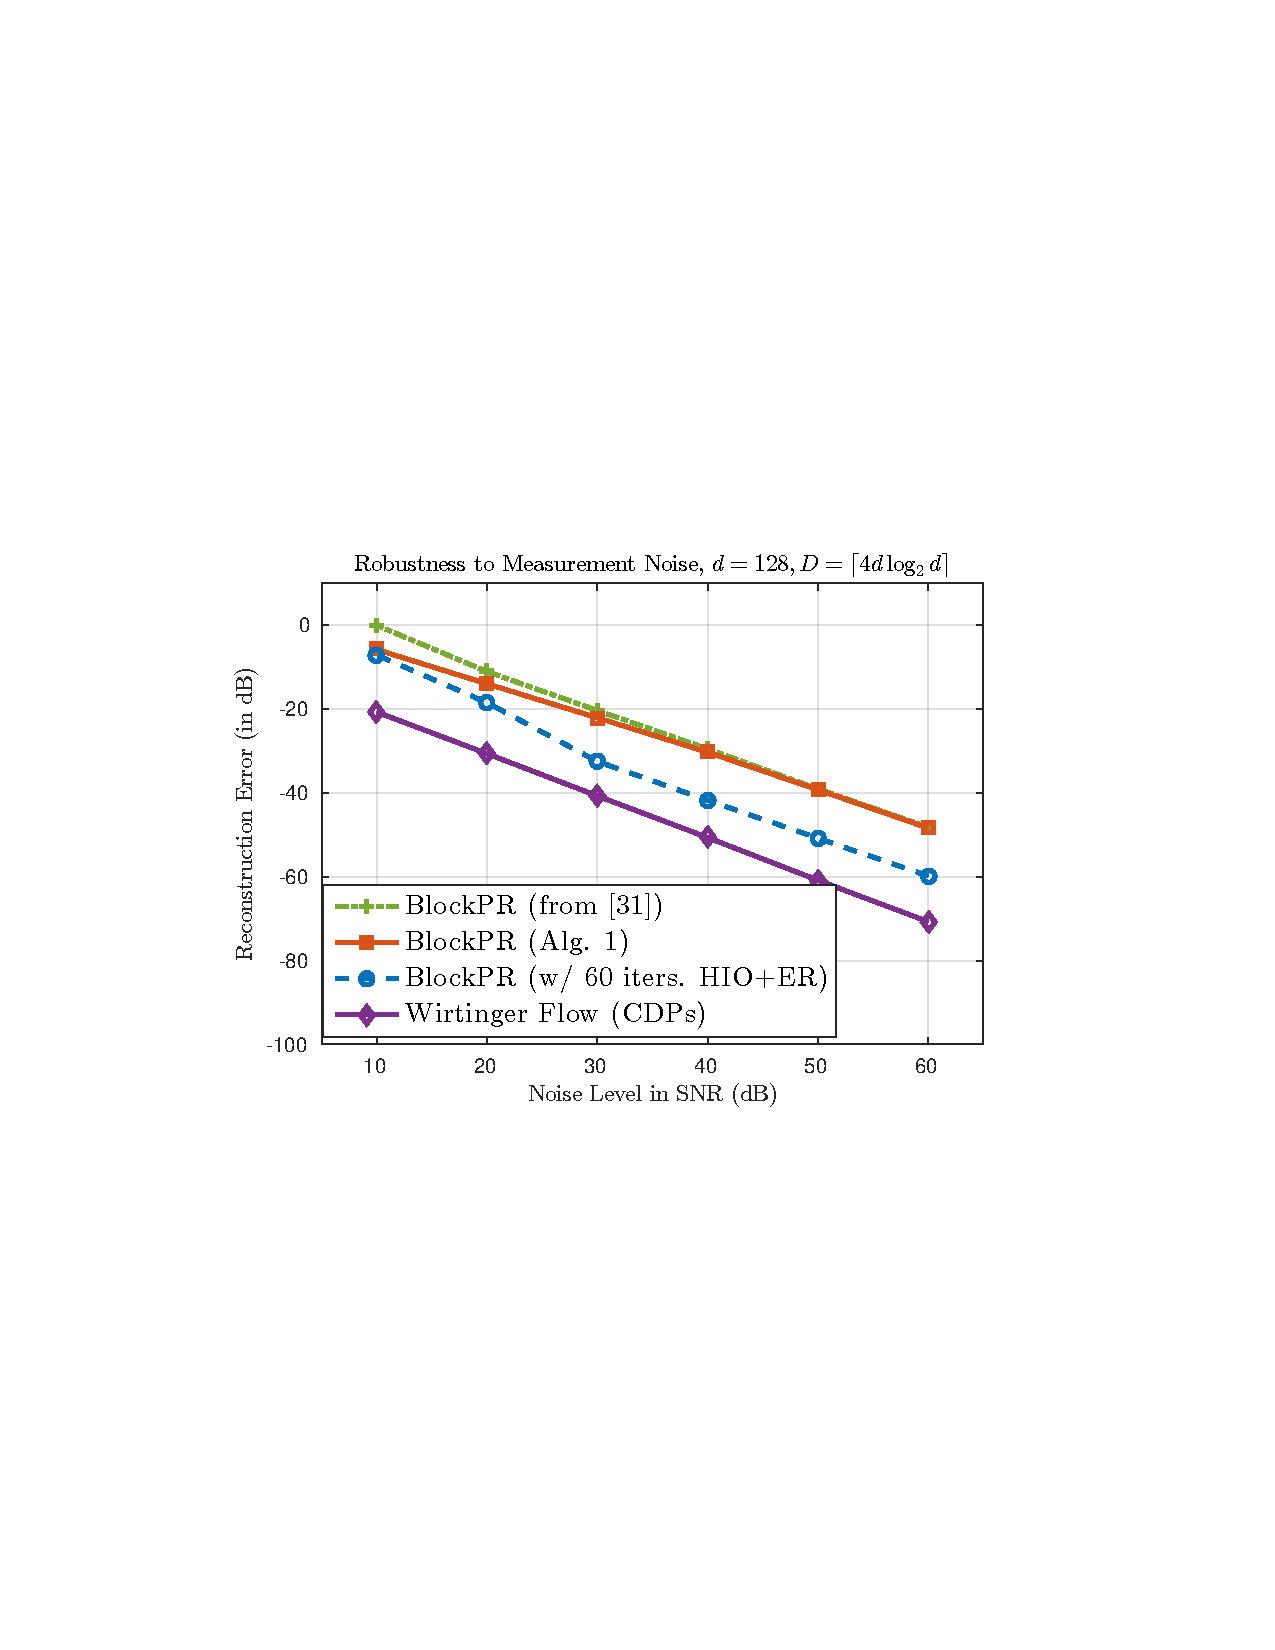
\includegraphics[clip=true, trim = 1.5in 3.5in 1.5in 3.25in,scale=0.610]{pics/fig2a}
\caption{Improved Robustness to Measurement Noise -- Comparing Variants of the {\em BlockPR}
algorithm}
\label{fig:eig_vs_greedy}
\end{subfigure}
\hfill
\begin{subfigure}[b]{0.495\textwidth}
\centering
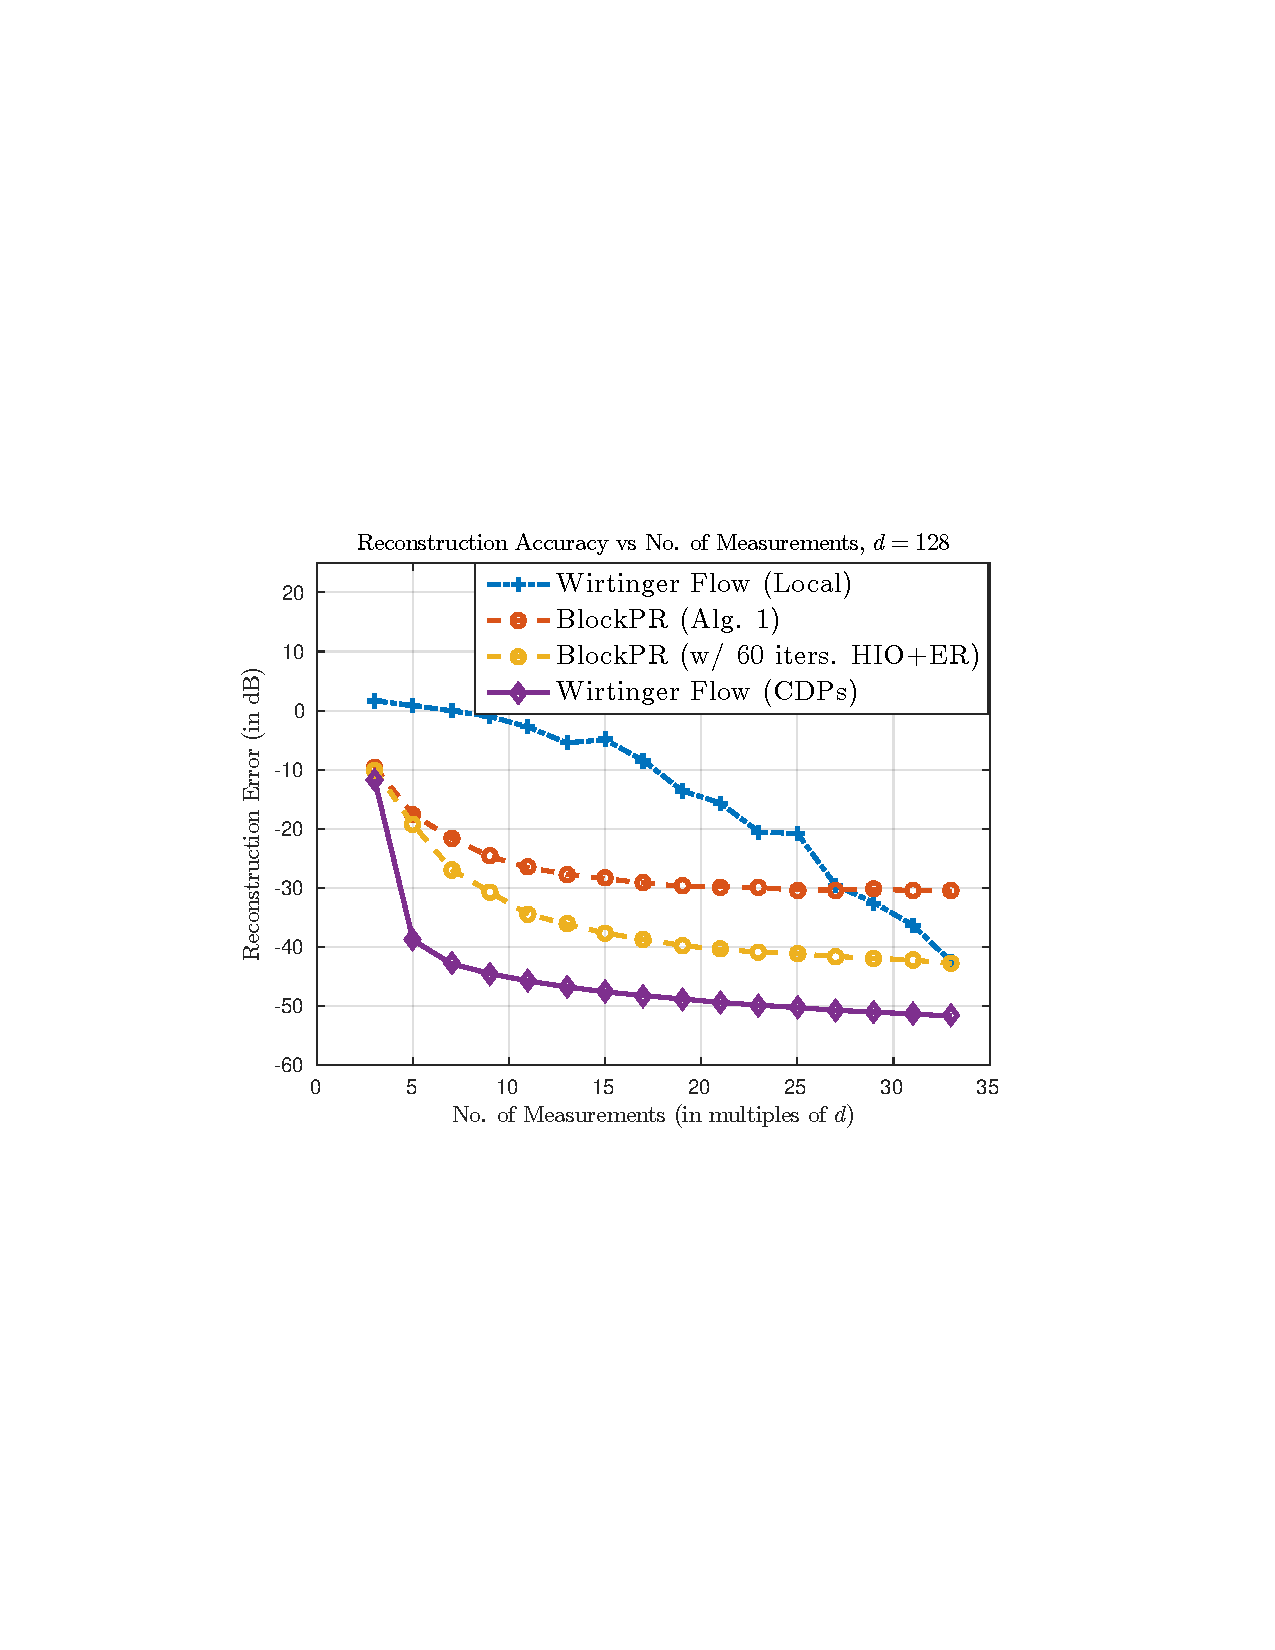
\includegraphics[clip=true, trim = 1.5in 3.35in 1.5in 3.25in,scale=0.565]{pics/fig2b}
\caption{Reconstruction Error vs. No. of Measurements; (Reconstruction at $40$dB SNR)}
\label{fig:WF_meas}
\end{subfigure}
\caption{Robust Phase Retrieval -- Local vs. Global Measurements}
\label{fig:WF}
\end{figure}
%


%SHOW PLOTS HERE, AND MENTION BRIEFLY THAT WE ARE TAKING THE MEAN OF THE DELTA MAGNITUDE ESTIMATES FOR EACH 
%$|(x_0)_j|$ PRODUCED BY THE TOP EIGENVECTORS OF $D_{j-\delta+1}, \dots, D_j$ IN OUR BETTER IMPLEMENTATION.  IN ADDITION, POST PROCESSING WITH <= 100 ITERATIONS OF ALTERNATING PROJECTIONS IS ALSO USED TO FURTHER IMPROVE OUR FINAL NUMERICAL NOISE ROBUSTNESS...\\
\subsection{Experiments with Measurements from Example 2 of \S \ref{sec:MeasMatrix}}
\label{sec:SparseMeasureMasks}

We begin by presenting results in Fig.~\ref{fig:eig_vs_greedy} demonstrating the improved noise
robustness of the proposed method over the formulation in \cite{IVW2015_FastPhase}. Recall that
\cite{IVW2015_FastPhase} uses a greedy angular synchronization method instead of the
eigenvector-based procedure analyzed in this paper. Fig.~\ref{fig:eig_vs_greedy} plots the
reconstruction error when recovering a $d=128$ length complex Gaussian test signal using $D=\lceil
4d\log_2 d\rceil$ measurements at different added noise levels. As mentioned above,
the local correlation measurements described in Example 2 of Section \ref{sec:MeasMatrix} are
utilized in this plot and in all the ensuing experiments in this subsection unless otherwise
indicated. Three variants of the proposed algorithm are plotted in Fig.~\ref{fig:eig_vs_greedy}:
\begin{enumerate}
    \item an implementation of Algorithm \ref{alg:phaseRetrieval1} (denoted by $\square$'s),
%    \item an implementation of Algorithm \ref{alg:phaseRetrieval1} with the improved magnitude estimation
%        procedure detailed in \S \ref{sec:MagEstImpNumerical} (with $s=1$ and using the average of the obtained $\tilde D_{j\prime}$
%        block magnitude estimates) and post-processed using $100$ iterations of the {\em
%        Gerchberg--Saxton} (or Error Reduction -- ER)
%        alternating projection algorithm (denoted by $\circ$'s), and 
    \item an implementation of Algorithm \ref{alg:phaseRetrieval1} post-processed using 
        $60$ iterations of the Hybrid Input--Output (HIO) and Error Reduction (ER) algorithms
        (implemented in two successive sets, with each set consisting of $20$ iterations of HIO followed 
        by $10$ ER iterations; denoted by $\circ$'s), and 
    \item the algorithmic implementation from \cite{IVW2015_FastPhase} (denoted by $+$'s). 
\end{enumerate}
%
We see that the eigenvector-based angular synchronization method proposed in this paper provides
more accurate reconstructions -- especially at low SNRs -- over the greedy angular synchronization
of \cite{IVW2015_FastPhase}. Moreover, post-processing using the HIO+ER algorithms as detailed above yields
a significant improvement in reconstruction errors over the two other variants. For reference, we also
include reconstruction errors with the {\em Wirtinger Flow} algorithm (denoted by $\Diamond$'s) when
using ({\em global}) coded diffraction pattern (CDP) measurements. Specifically, we use $2\delta-1$
(with $\delta = 2\log_2d = 14$) octanary modulations/codes as described in \cite[\S 1.5,
(1.9)]{Candes2014WF} to construct the CDP measurements. Clearly, using global measurements such as
coded diffraction patterns provides superior noise tolerance; however, they are not applicable to
the local measurement model considered here.  Indeed, when the {\em Wirtinger Flow} algorithm is
used with local measurements such as those described in this paper, the noise tolerance
significantly deteriorates. Fig. \ref{fig:WF_meas} illustrates this phenomenon by plotting the
reconstruction error in recovering a $d=128$ length complex Gaussian test signal at $40$~dB SNR when
using different numbers of measurements, $D$. {\em Wirtinger flow}, for example, requires a large
number of local measurements before returning accurate reconstructions. 
%We conjecture that the spectral initialization used in {\em
%Wirtinger Flow} and devised for
%global measurements (random Gaussian and coded diffraction pattern measurements) is less effective
%when applied to local measurements such as those considered in this paper. 
The wide disparity in reconstruction accuracy between local and global measurements for {\em
Wirtinger Flow} illustrates the significant challenge in phase retrieval from local measurements.
Furthermore, we see that the {\em BlockPR} method proposed in this paper is more noise tolerant than
{\em Wirtinger Flow} for local measurements.
%
\begin{figure}[hbtp]
\centering
\begin{subfigure}[b]{0.495\textwidth}
\centering
%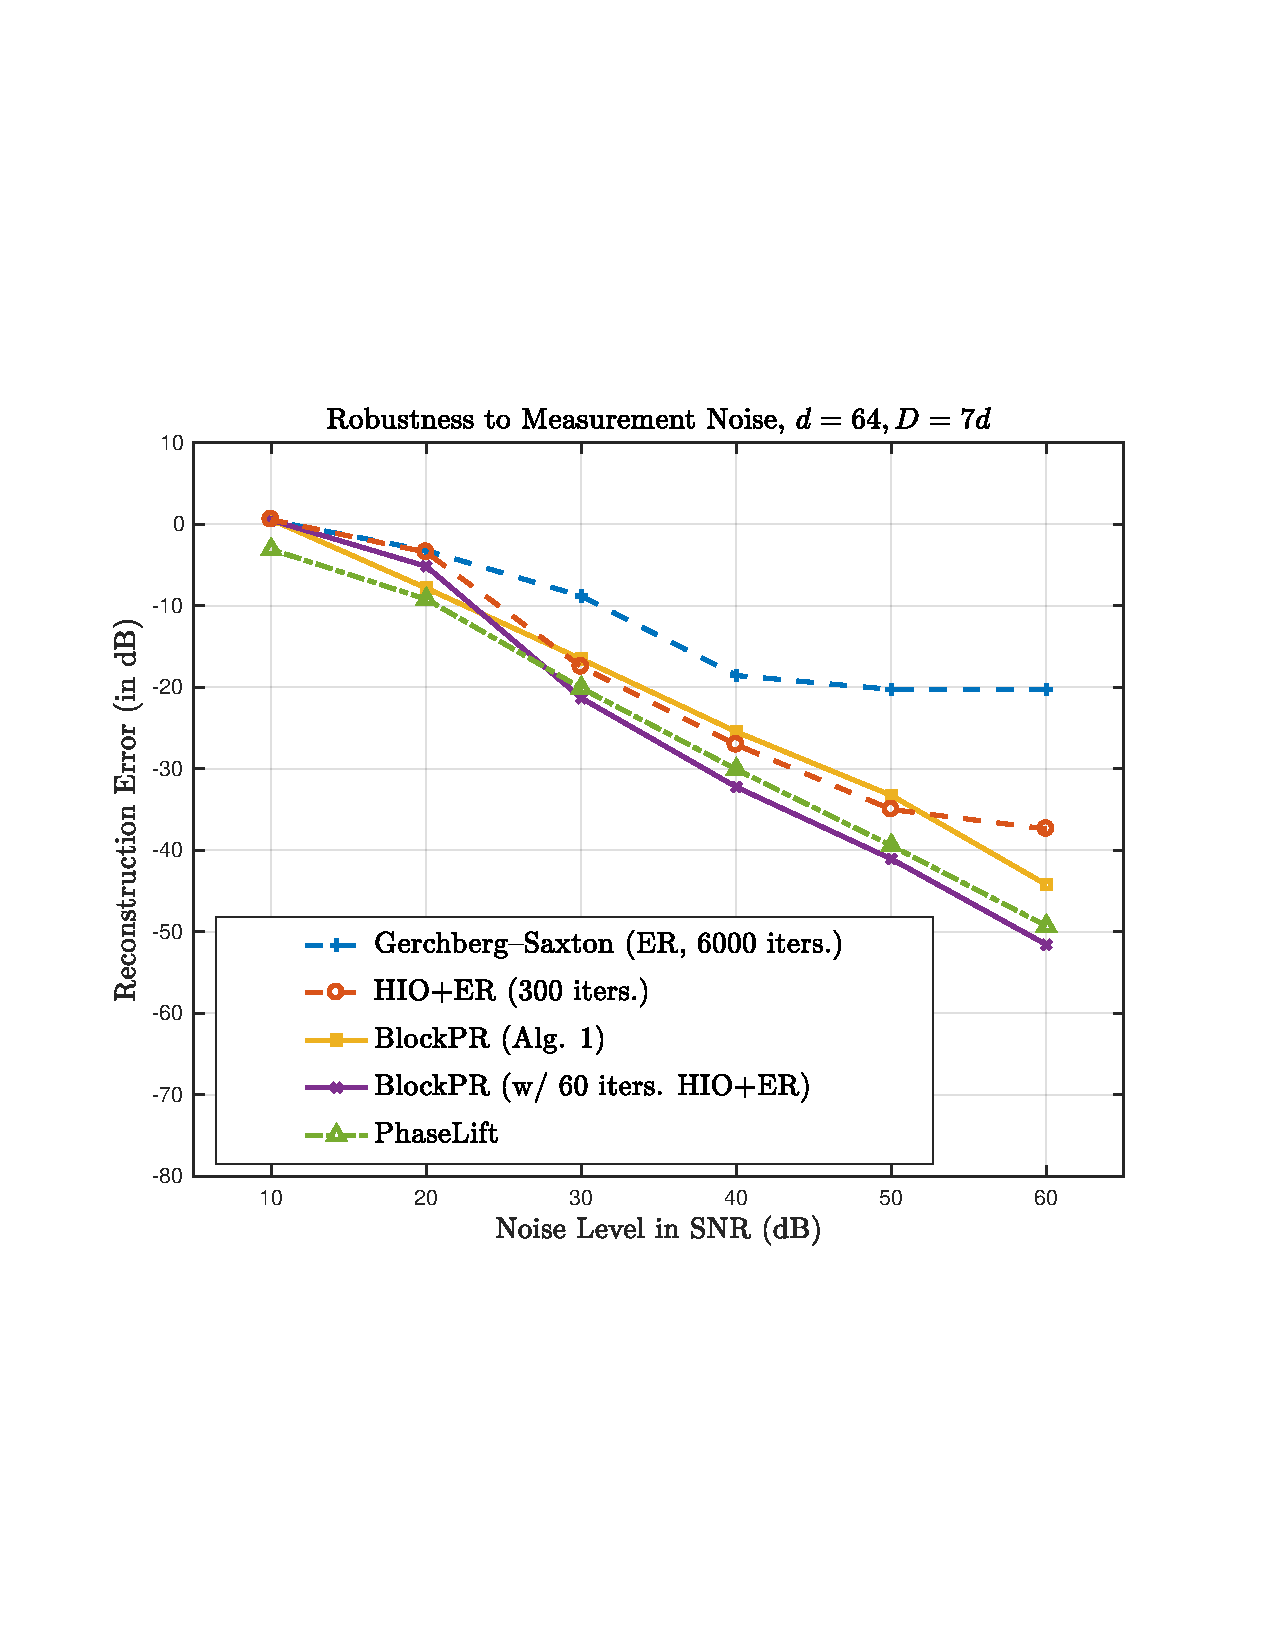
\includegraphics[clip=true, trim = 0.75in 2.75in 1in 2.5in,scale=0.45]{pics/fig3a}
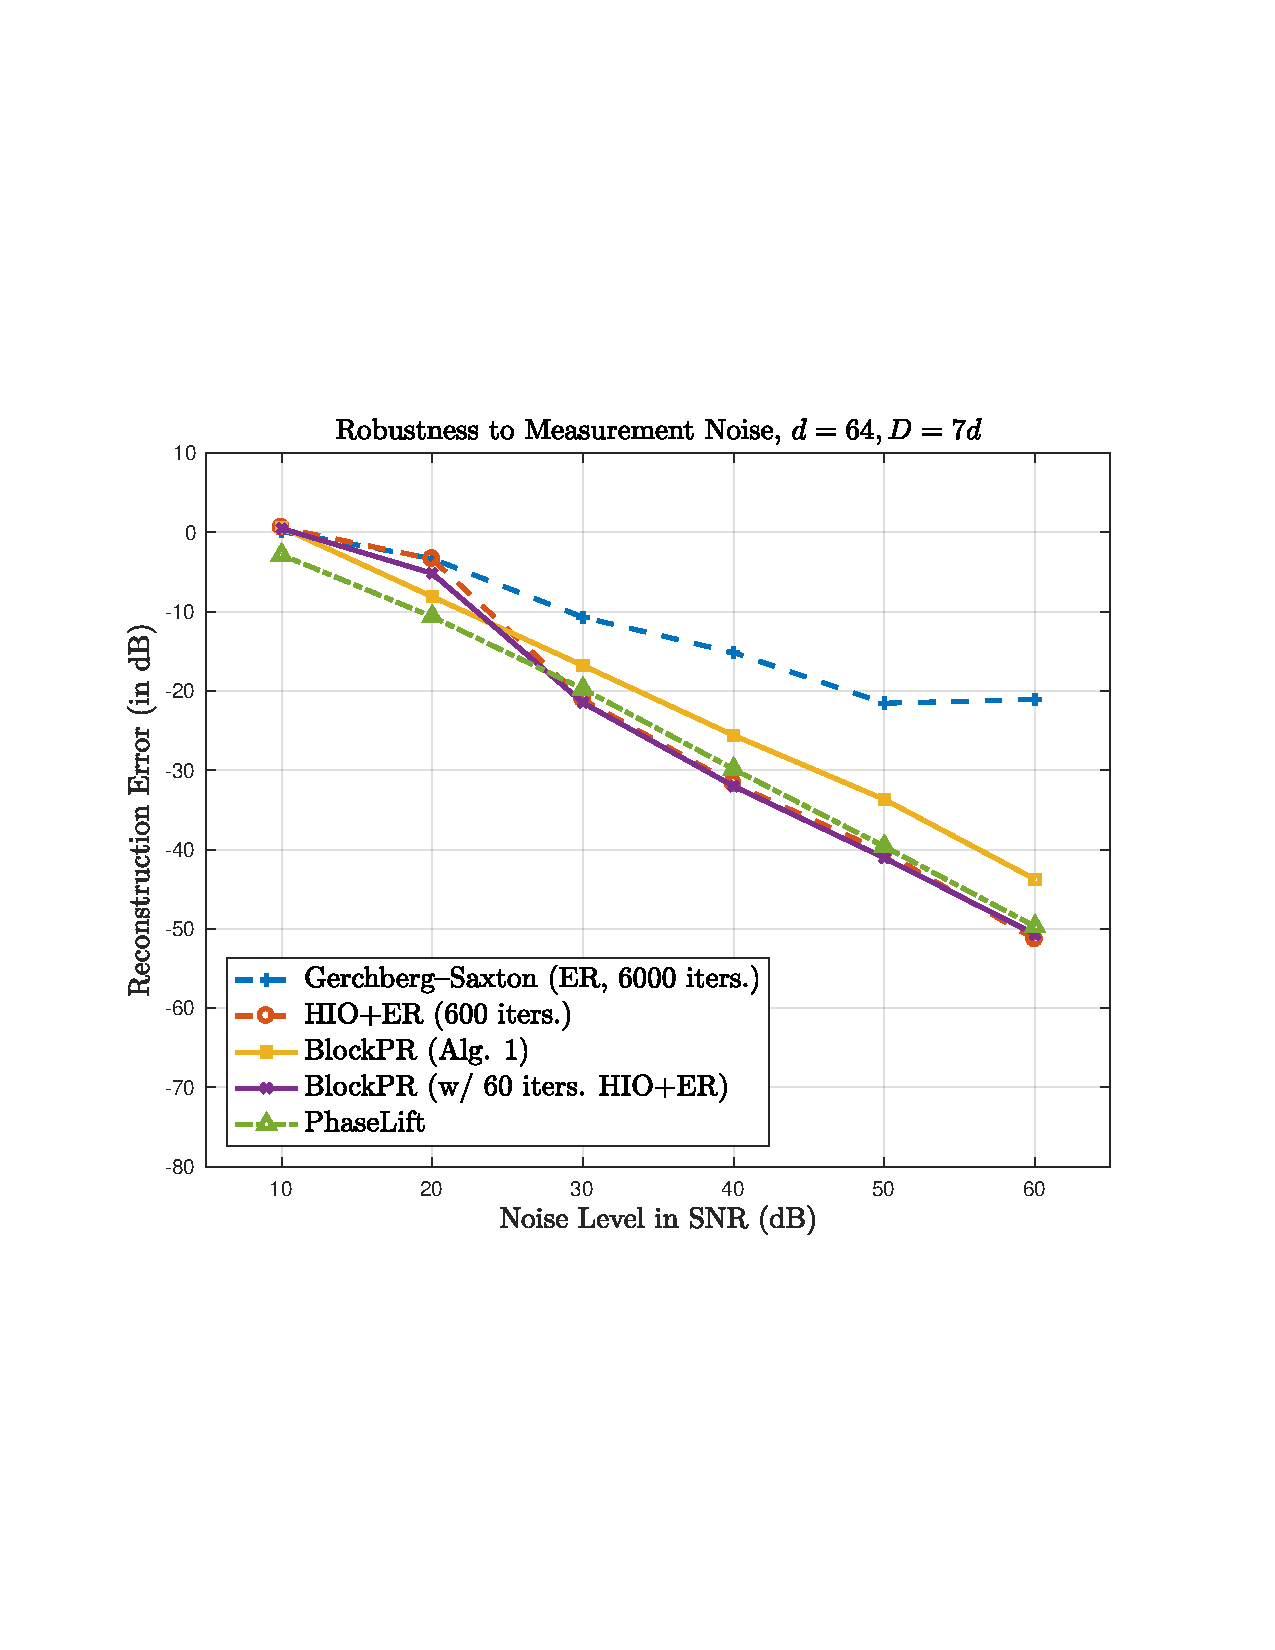
\includegraphics[clip=true, trim = 0.75in 2.75in 1in 2.5in,scale=0.45]{pics/robustness_600a}
\caption{Using $D=7d$ measurements.}
\label{fig:noise-7d}
\end{subfigure}
\hfill
\begin{subfigure}[b]{0.495\textwidth}
\centering
%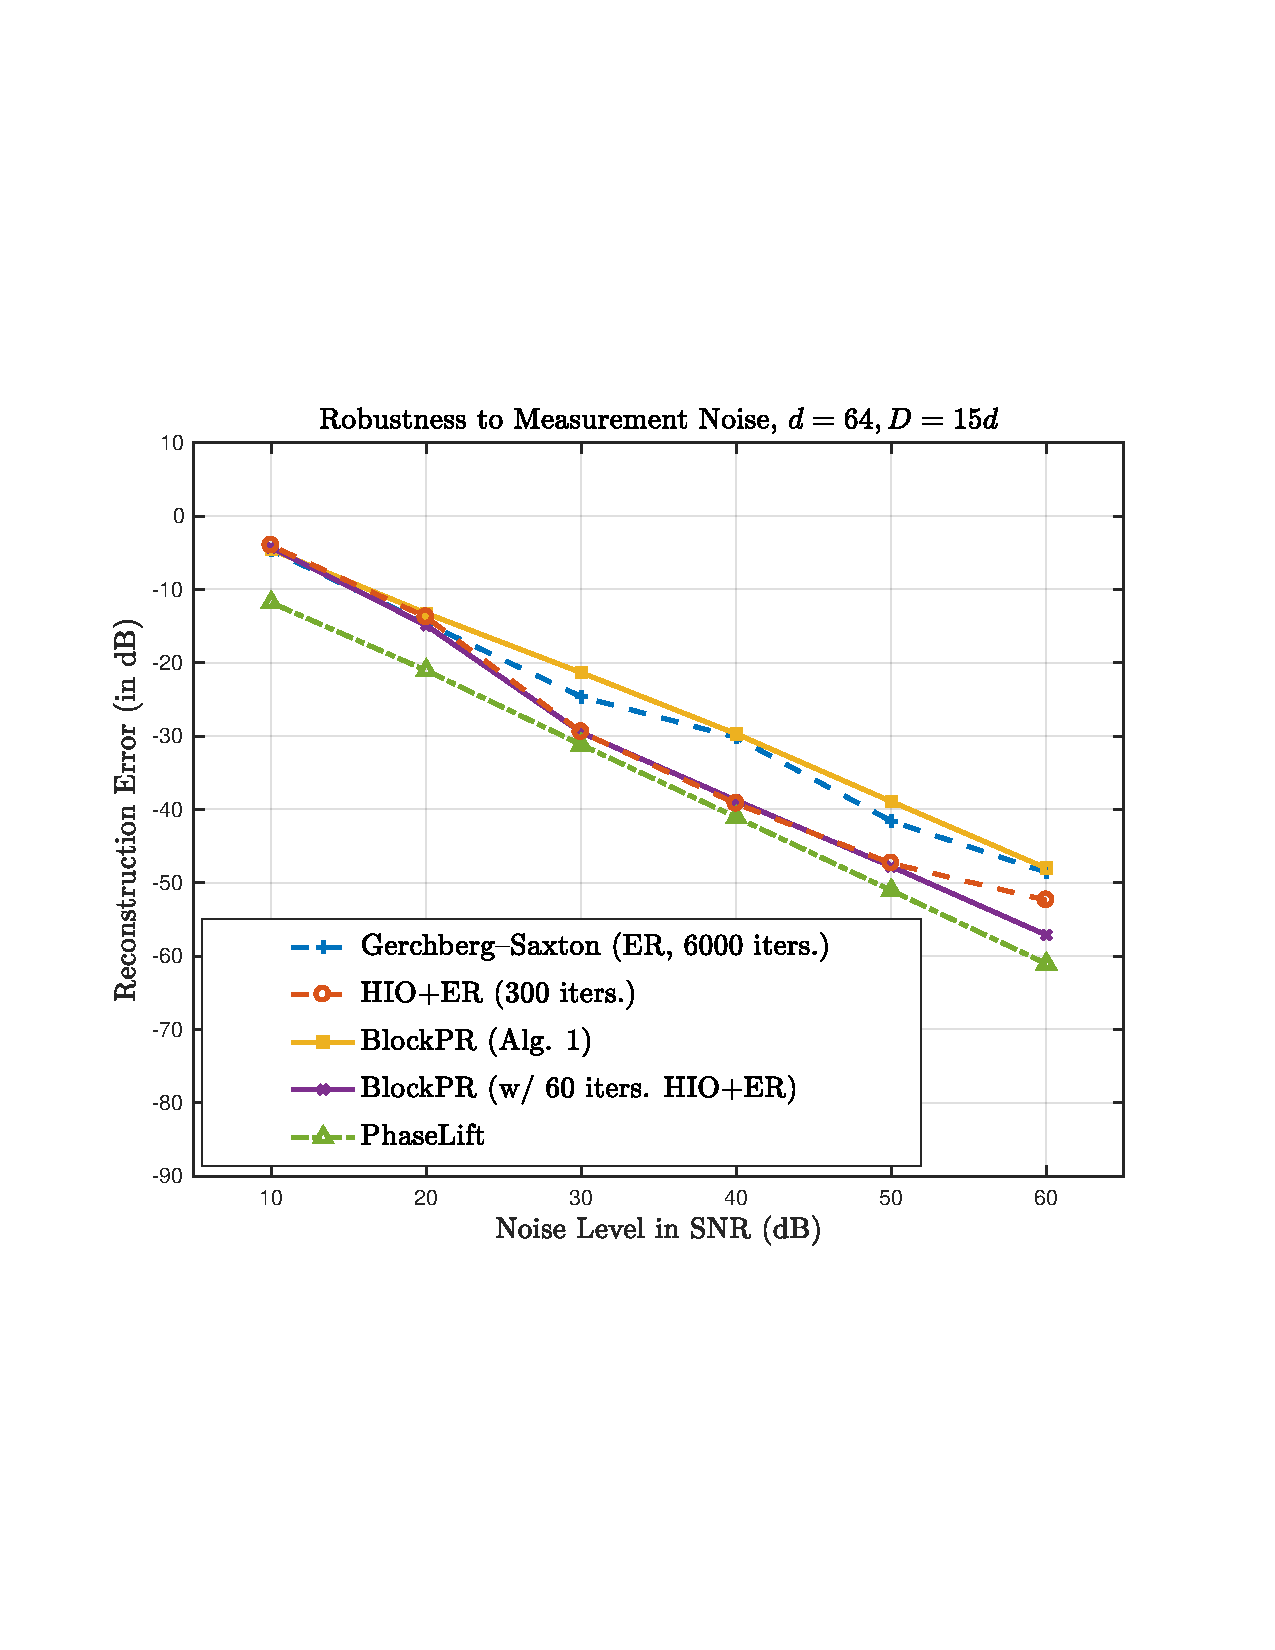
\includegraphics[clip=true, trim = 0.75in 2.75in 1in 2.5in,scale=0.45]{pics/fig3b}
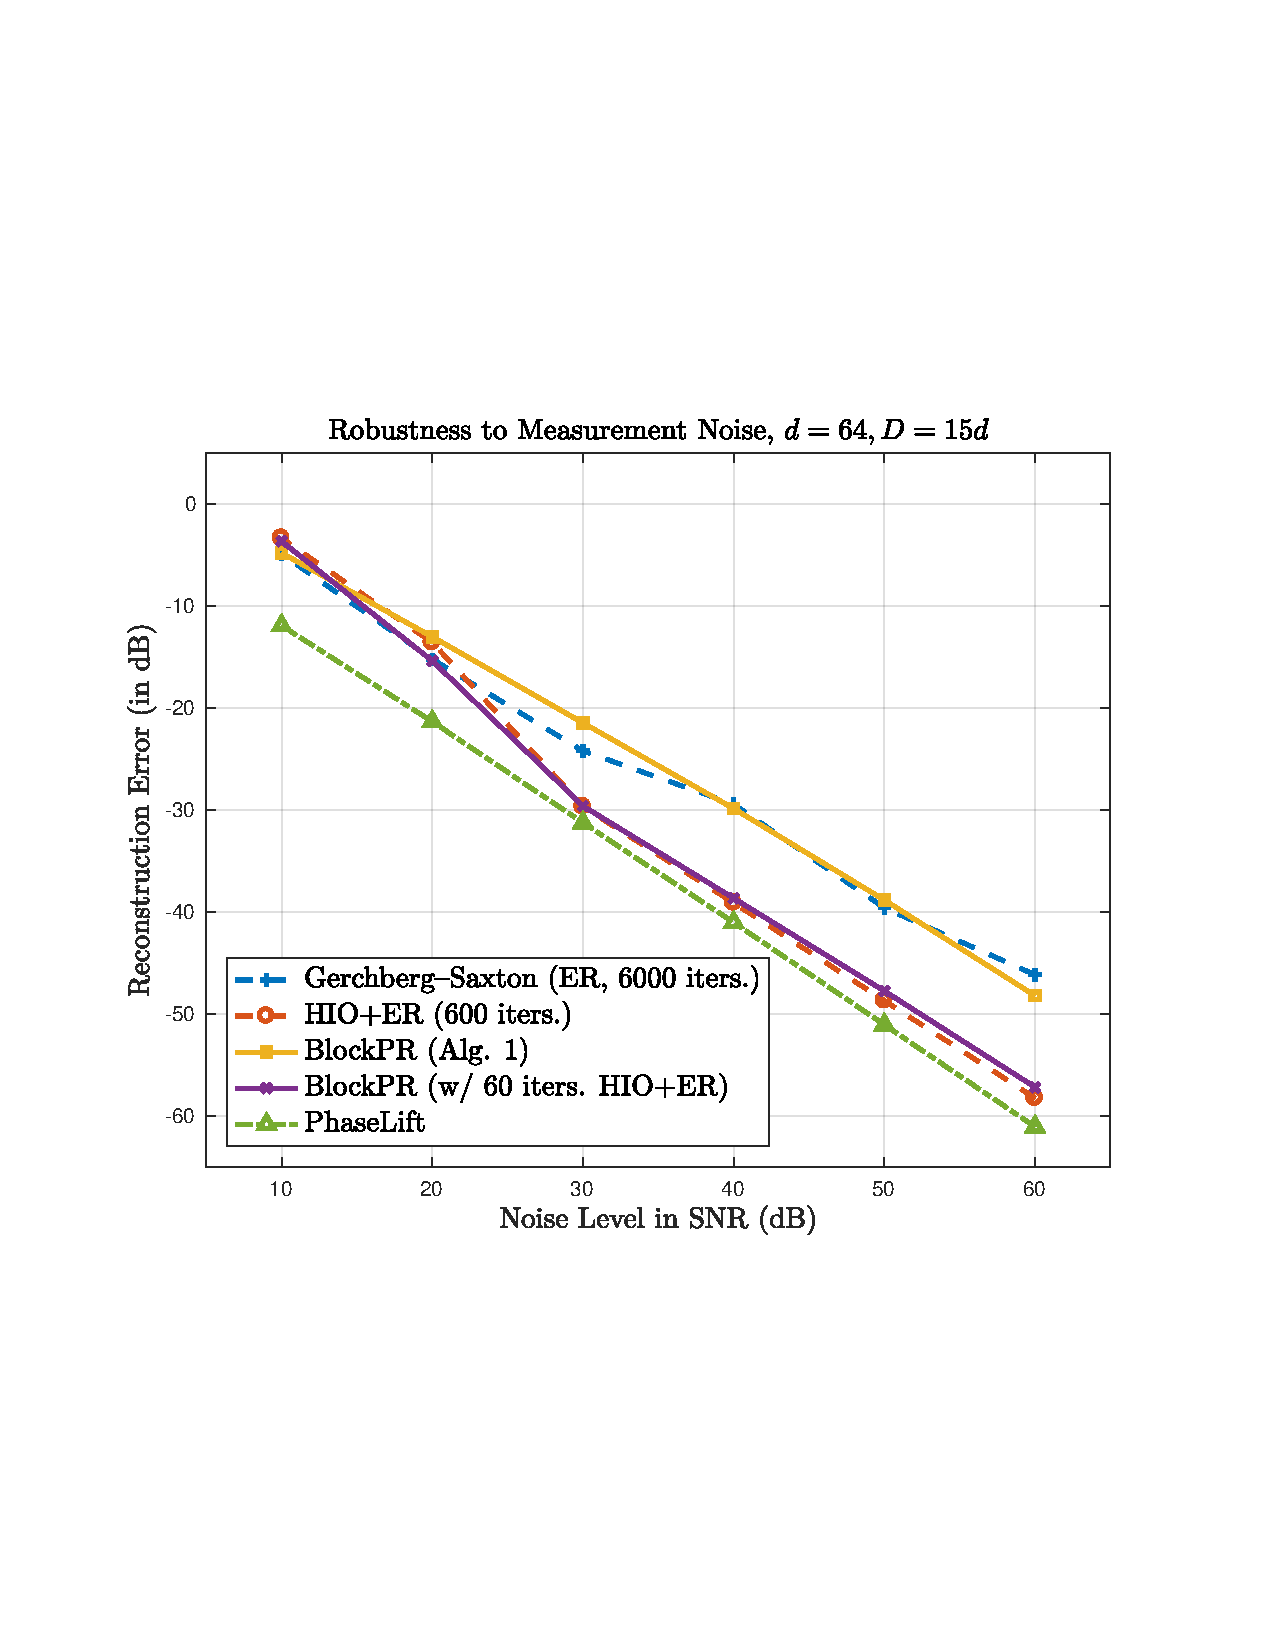
\includegraphics[clip=true, trim = 0.75in 2.75in 1in 2.5in,scale=0.45]{pics/robustness_600b}
\caption{Using $D=15d$ measurements.}
\label{fig:noise-15d}
\end{subfigure}\vspace{0.1in} \\
\begin{subfigure}[b]{0.495\textwidth}
\centering
%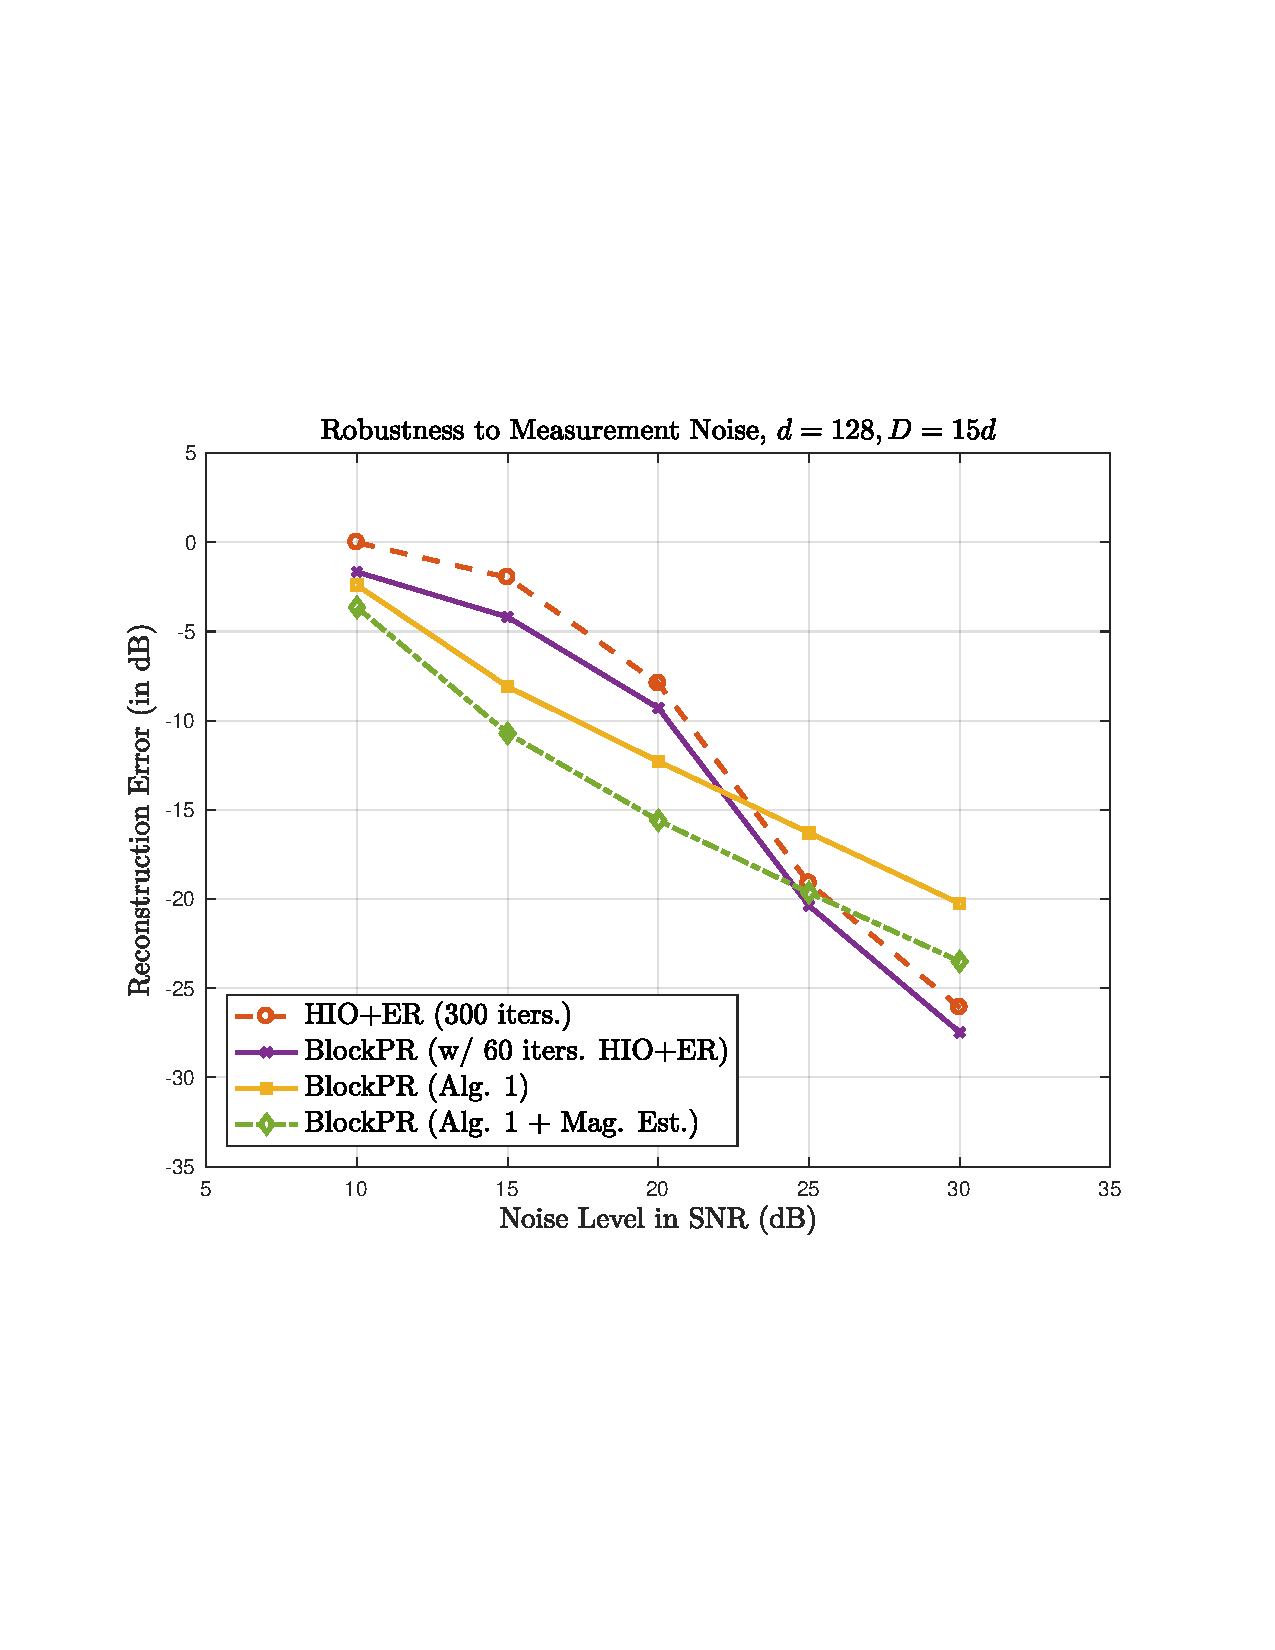
\includegraphics[clip=true, trim = 0.75in 2.75in 1in 2.5in,scale=0.45]{pics/fig3c}
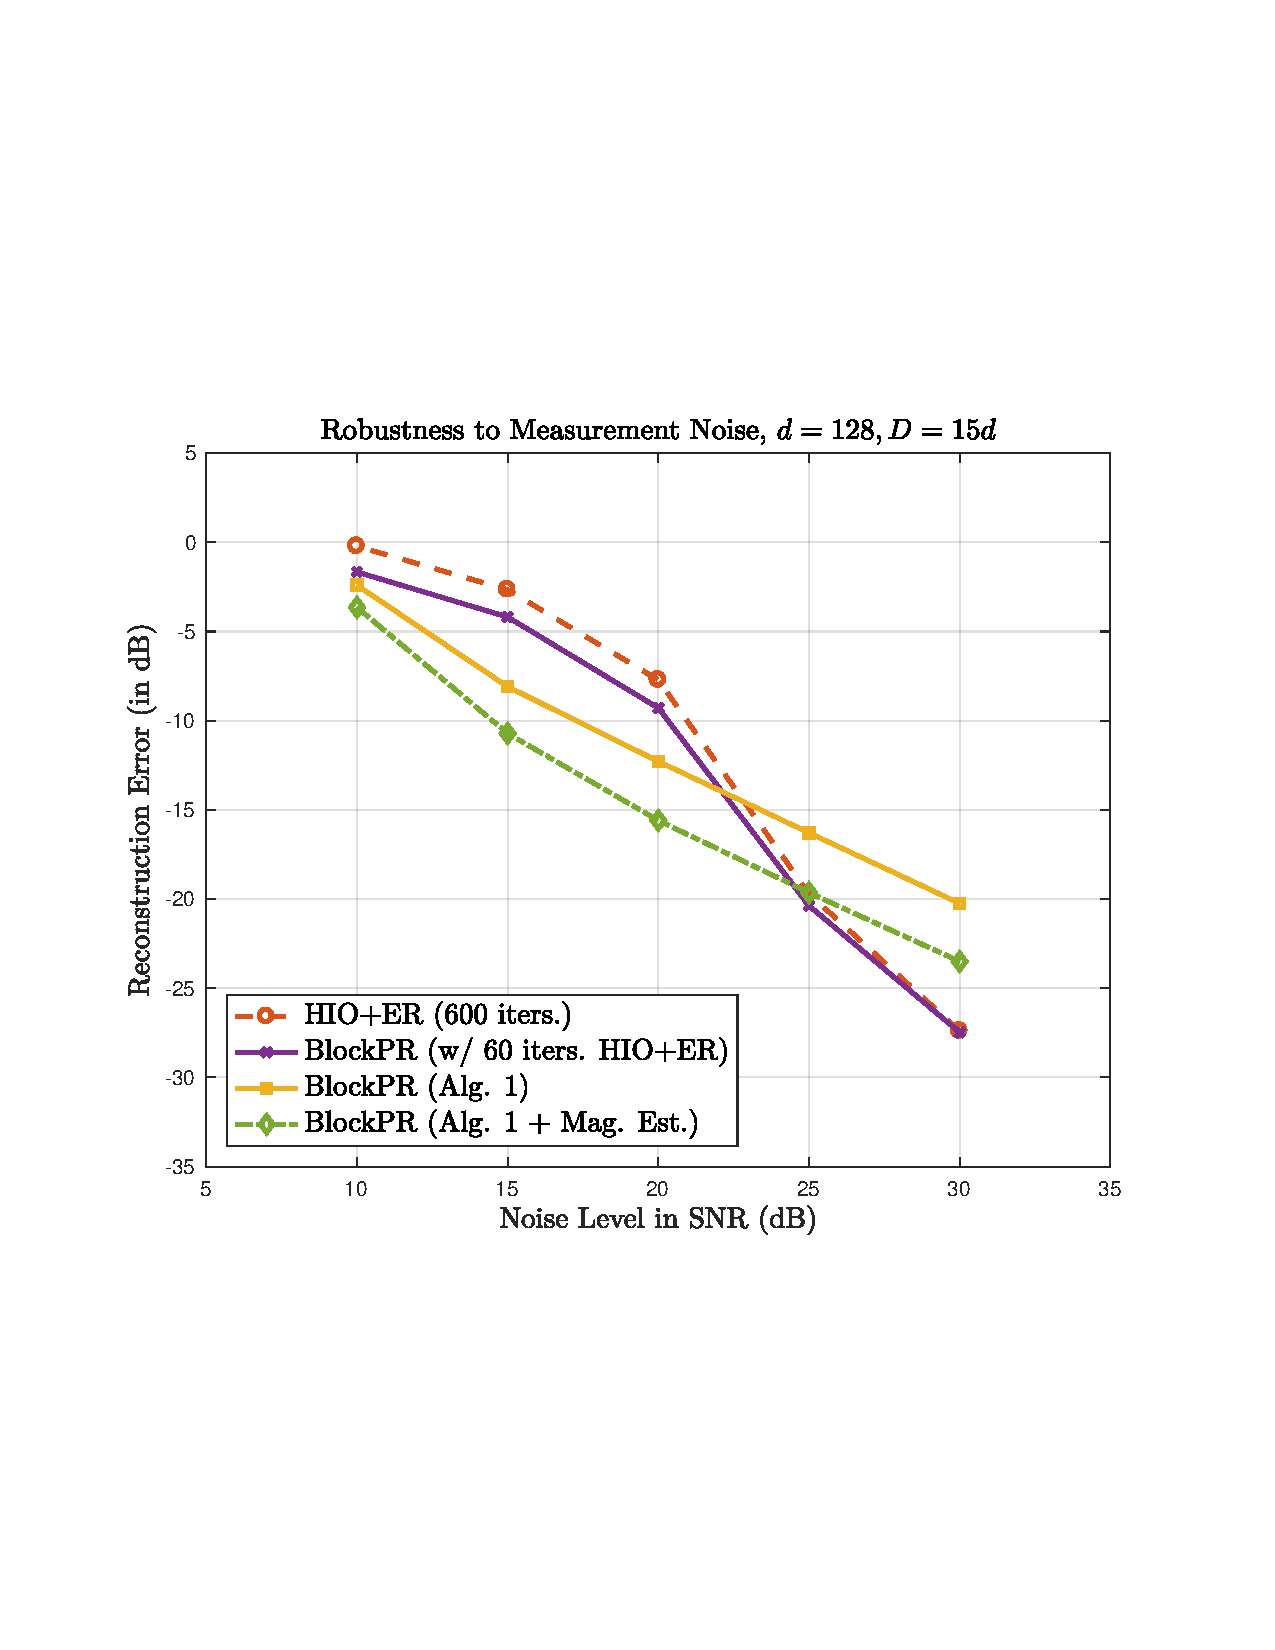
\includegraphics[clip=true, trim = 0.75in 2.75in 1in 2.5in,scale=0.45]{pics/robustness_600c}
\caption{Low SNR Simulations: Using $D=15d$ measurements, Problem Size $d=128$}
\label{fig:lowsnr_128}
\end{subfigure}
\hfill
\begin{subfigure}[b]{0.495\textwidth}
\centering
%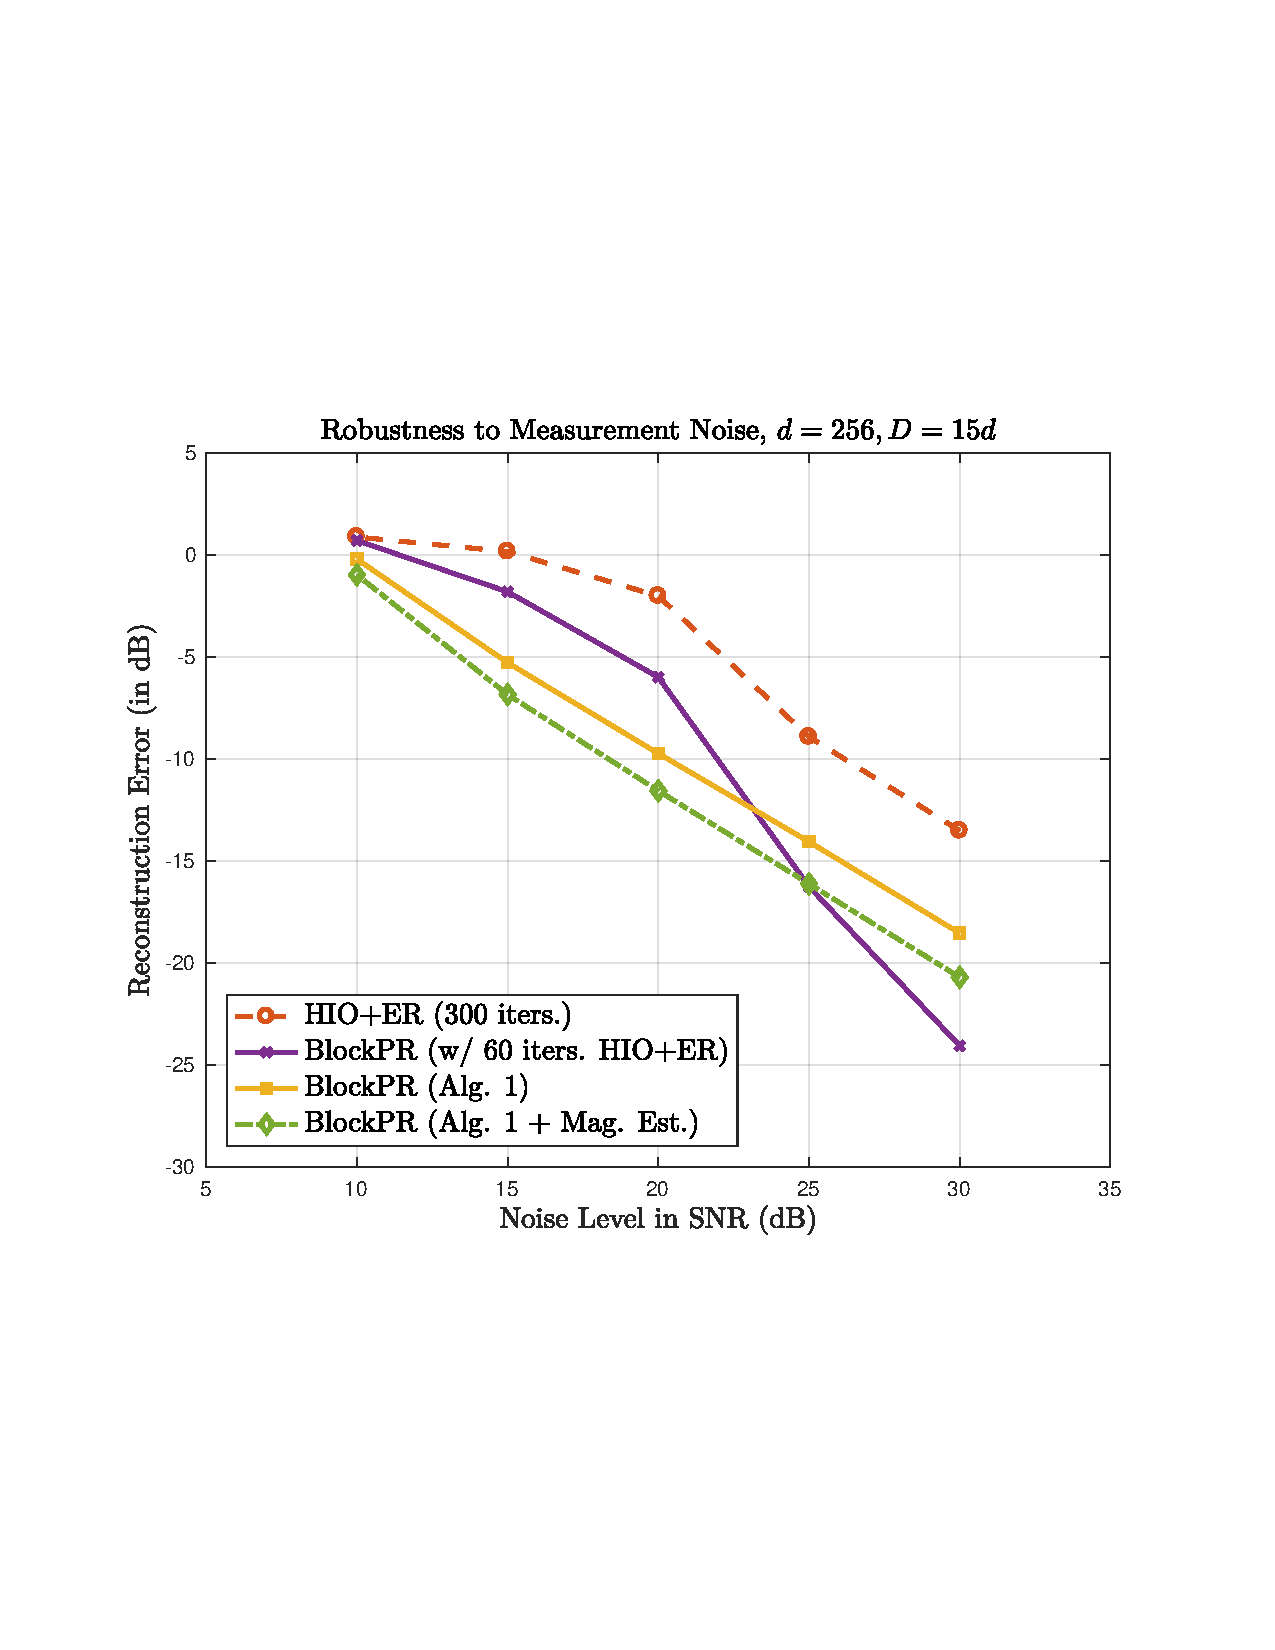
\includegraphics[clip=true, trim = 0.75in 2.75in 1in 2.5in,scale=0.45]{pics/fig3d}
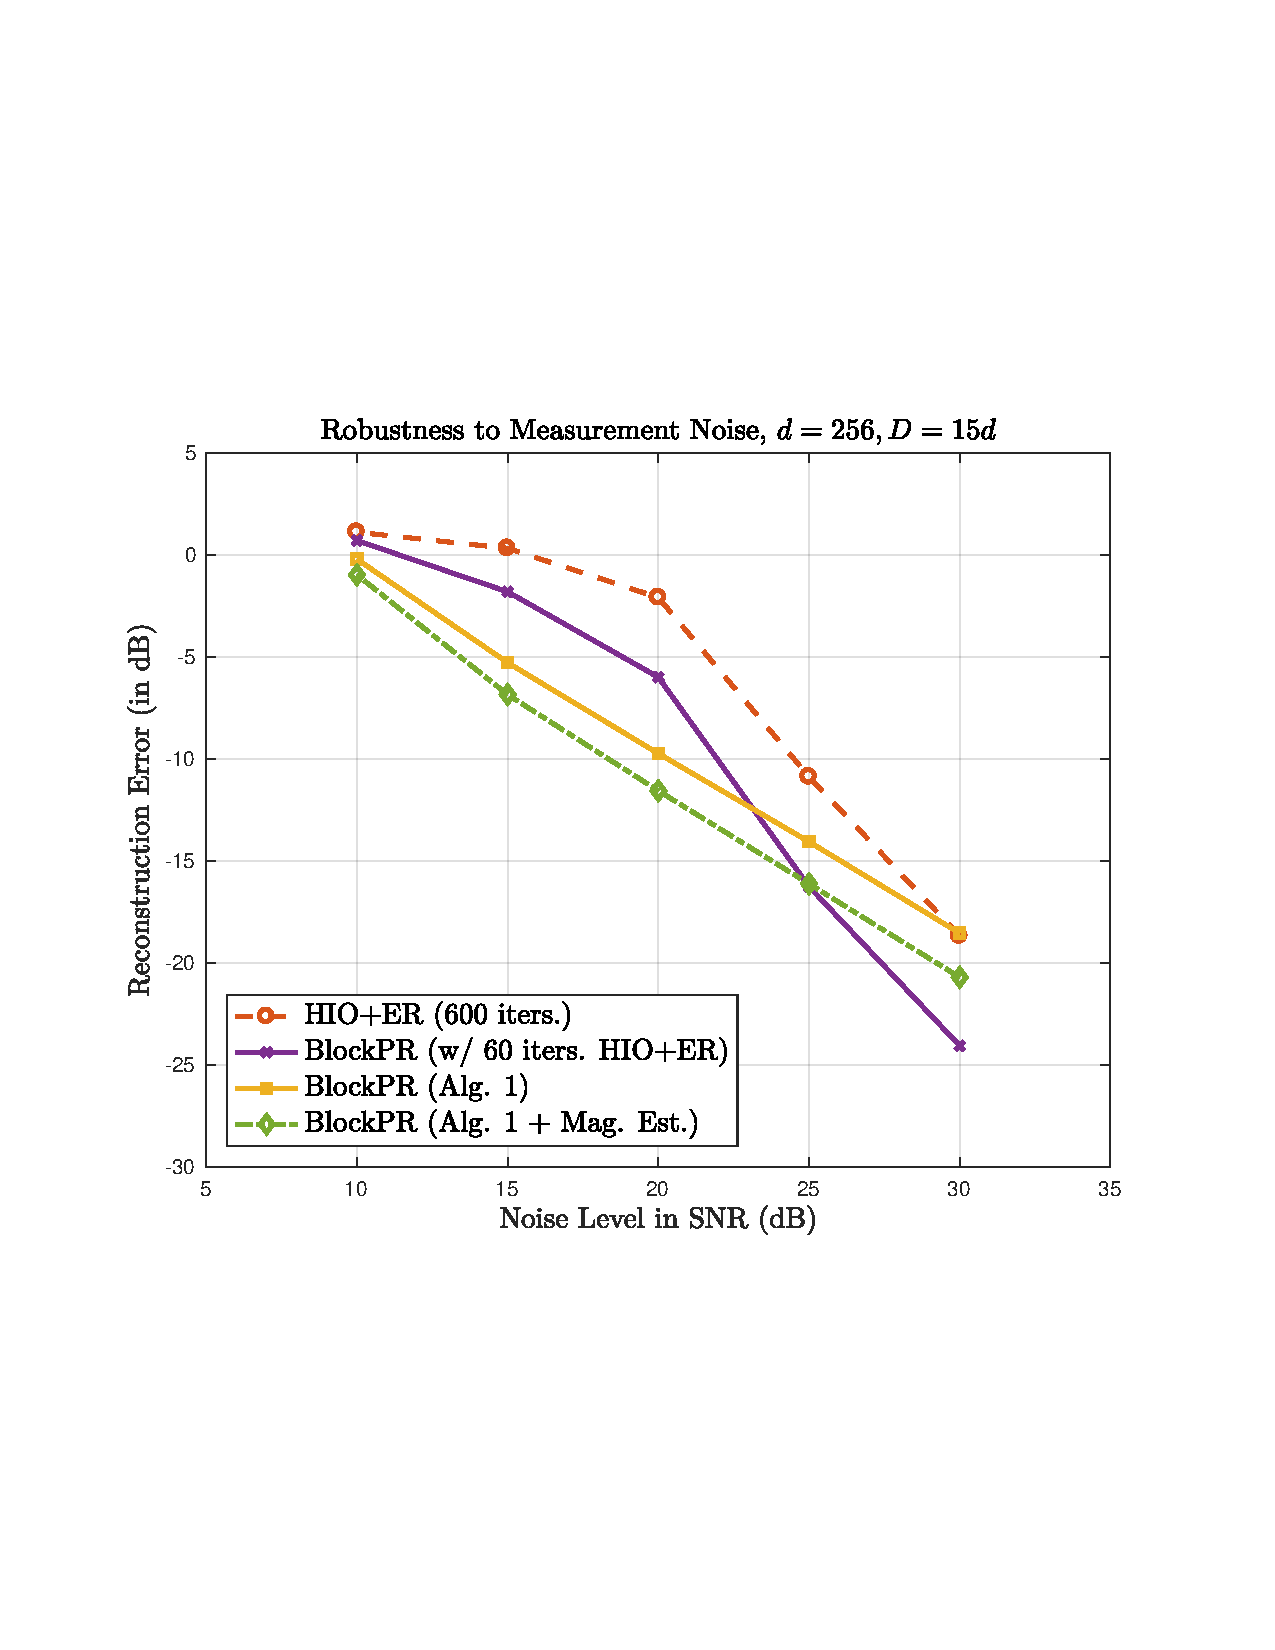
\includegraphics[clip=true, trim = 0.75in 2.75in 1in 2.5in,scale=0.45]{pics/robustness_600d}
\caption{Low SNR Simulations: Using $D=15d$ measurements, Problem Size $d=256$}
\label{fig:lowsnr_256}
\end{subfigure}
\caption{Robustness to measurement noise -- Phase Retrieval from 
deterministic local correlation measurements.}
\label{fig:noise-local}
\end{figure}
%
%\subsection{Robustness to Measurement Noise}
%\label{sec:numeval-noise}

Given the weaker performance of {\em Wirtinger Flow} with local measurements, we now restrict our attention to the empirical evaluation of the proposed method (Alg. \ref{alg:phaseRetrieval1}, as well as the post-processed variant (with HIO+ER iterations)) against {\em PhaseLift} and alternating projection algorithms. Although numerical simulations suggest that these methods work with local measurements, we note that (to the best of our knowledge) there are no theoretical recovery or robustness guarantees for these methods and measurements.  The {\em PhaseLift} algorithm was implemented as a trace regularized least-squares problem using CVX \cite{cvx,gb08} -- a package for specifying and solving convex programs in Matlab. We consider two variants from the family of alternating projection methods -- {\em Gerchberg--Saxton} (sometimes referred to as the Error Reduction (ER) algorithm) and Hybrid Input-Output (HIO). For both algorithms, the following two projections were utilized: (i) projection onto the measured magnitudes, and (ii) projection onto the span of the measurement vectors $\{\a_j\}_{j=1}^D$. This formulation as well as other details and connections to convex optimization theory can be found in \cite{bauschke2002phase}. For the ER and HIO implementations, the initial guess was set to be the all-zero vector.\footnote{\ We note that using a random starting guess does not change the qualitative nature of the empirical results.} For the HIO implementation, as is popular practice (see, for example, \cite{fienup1982comparison}) every few ($20$) HIO iterations were followed by a small number of ($10$) ER iterations, with the maximum number of HIO+ER iterations limited to $600$ -- this choice of iteration count ensures convergence of the algorithm (see Fig. \ref{fig:iter_HIOER}) while comparing favorably with the computational cost (see Fig. \ref{fig:exectime}) of the proposed {\em BlockPR} method. For the ER implementation, $6,000$ iterations were necessary to ensure convergence.

%-------------------------------------------------------
\begin{figure}[H]
    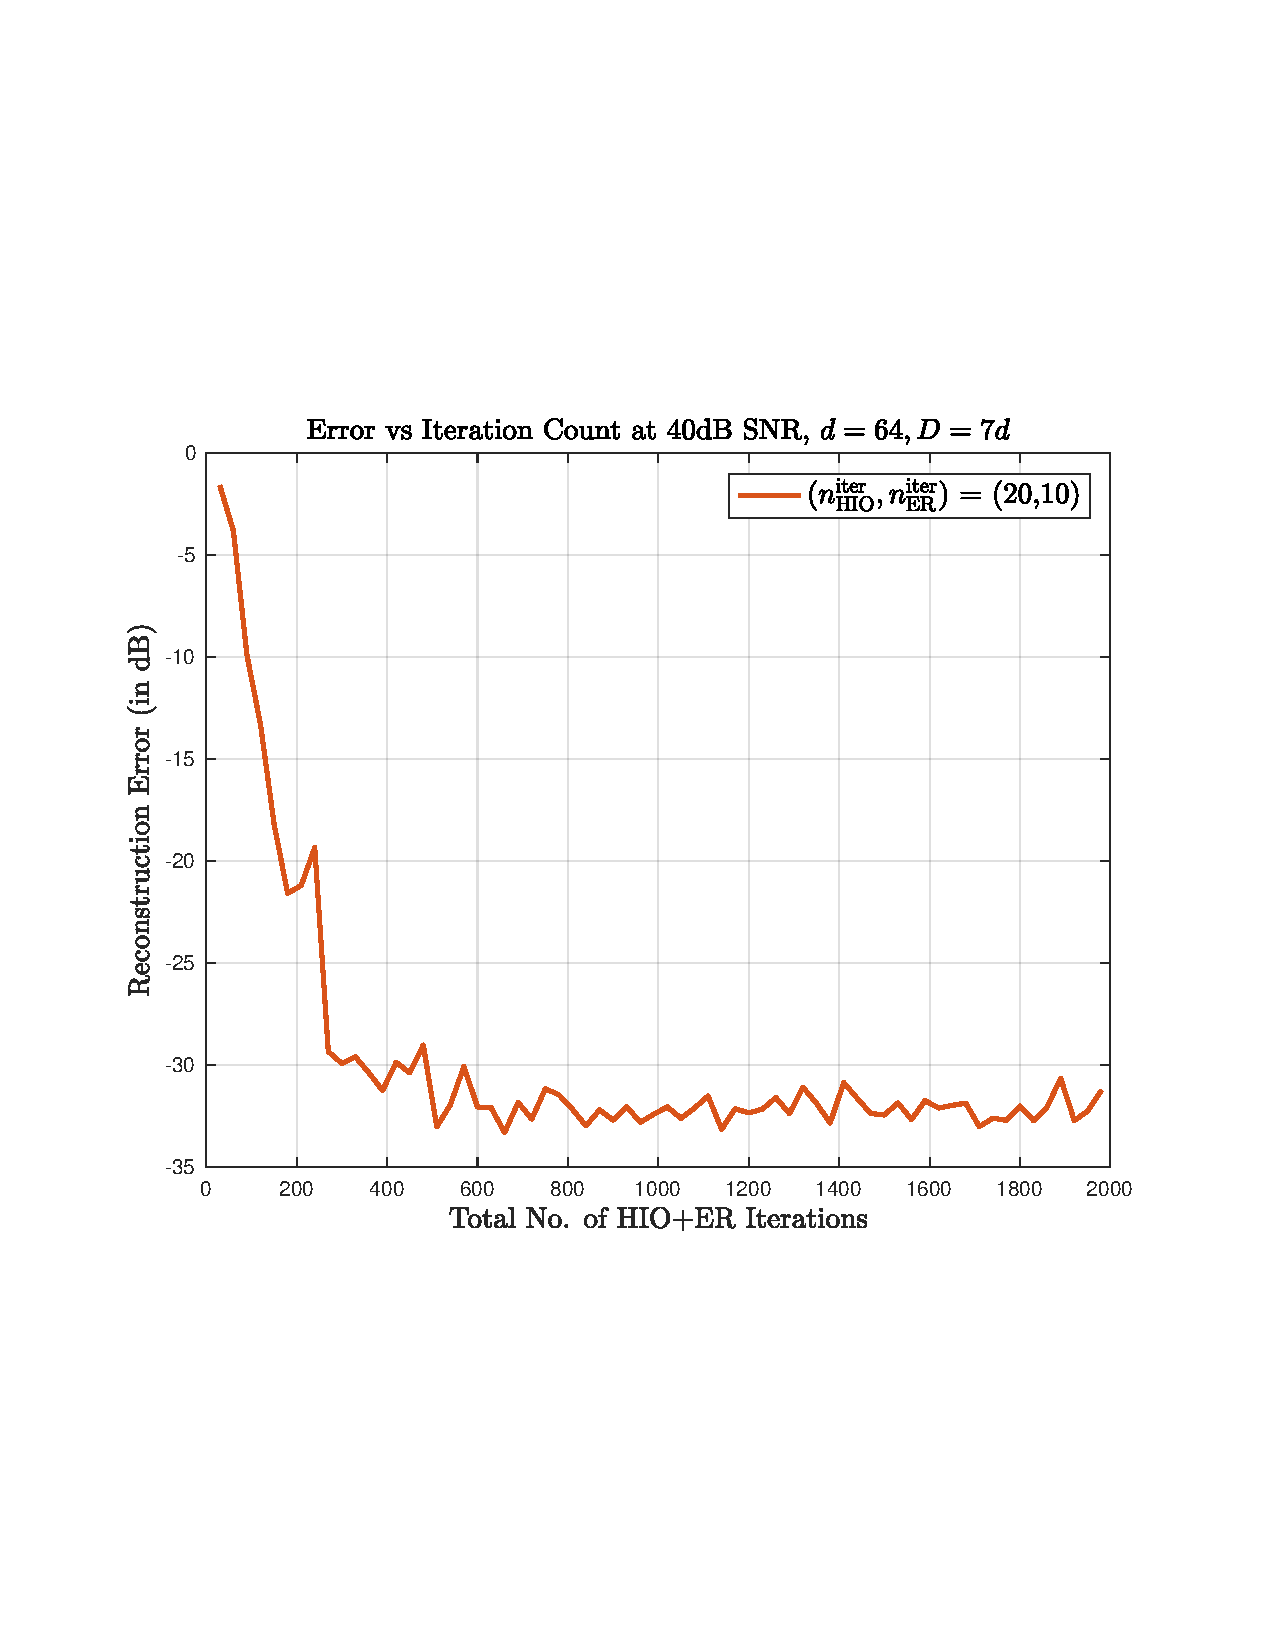
\includegraphics[clip=true, trim = 0.75in 2.75in 1in 2.75in,scale=0.45]{pics/err_iteration_count}
    \caption{Reconstruction Error vs. Iteration Count for HIO+ER Implementation}
    \label{fig:iter_HIOER}
\end{figure}
%-------------------------------------------------------

%SIMPLIFIED IN PARENTHESIS ABOVE?
%We refer the interested reader to \cite{bauschke2002phase} for an analysis
%of various alternating projection algorithms (including the aforementioned ER and HIO) from a convex
%optimization perspective -- our implementation of ER and HIO is inspired by this. 

We begin by presenting numerical results evaluating the robustness to measurement noise.  Figs.
\ref{fig:noise-7d} and \ref{fig:noise-15d} plot the error in reconstructing a $d=64$ length complex
vector $\x_0$ using $D=7d$ and $D=15d$ local correlation-based phaseless measurements respectively.
Note that this corresponds to using $\delta=4$ (and the associated $2\delta-1=7$ masks) and
$\delta=8$ (and the corresponding $2\delta-1=15$ masks) respectively. Moreover, the well-conditioned
{\em deterministic} (and sparse) measurement construction defined in Example 2 of Section
\ref{sec:MeasMatrix} was utilized along with additive Gaussian measurement noise. We see from Fig.
\ref{fig:noise-local} that the method proposed in this paper (denoted {\em BlockPR} in the figure)
performs reliably across a wide range of SNRs and compares favorably against existing popular phase
retrieval algorithms. When using a small number of measurements (as in Fig.  \ref{fig:noise-7d}, and
modeling real-world situations), both variants of the proposed method -- Alg.
\ref{alg:phaseRetrieval1}, as well as Alg.  \ref{alg:phaseRetrieval1} post-processed using $60$
HIO+ER iterations -- outperform the ER algorithm by significant margins and compare well with the 
popular HIO+ER algorithm. When more measurements are available (as in Fig.
\ref{fig:noise-15d}), the performance of the ER and HIO+ER algorithms approaches the performance of the
{\em BlockPR} variants proposed in this paper. In addition, the proposed methods also compare well
with the significantly more expensive {\em PhaseLift} reconstructions. We emphasize that the
superior performance of the proposed methods demonstrated here comes with rigorous theoretical
recovery guarantees for local measurements -- something that cannot
be said of any of the other methods in Fig.~\ref{fig:noise-local}. 

Additionally, Figs. \ref{fig:lowsnr_128} and \ref{fig:lowsnr_256} compare the performance of the
HIO+ER algorithm at low SNRs for problems sizes $d=128$ and $d=256$ respectively, with the various
{\em BlockPR} implementations -- including one with the improved magnitude estimation procedure
detailed in \S \ref{sec:MagEstImpNumerical} (with $s=1$ and using the average of the obtained
$\tilde D_{j\prime}$ block magnitude estimates). These figures demonstrate the value of the
magnitude estimation procedure from \S \ref{sec:MagEstImpNumerical} at low SNRs over the HIO+ER
post-processing method utilized in the other figures (and over the HIO+ER algorithm); we defer a
more detailed study of this to future work.

%
\begin{figure}[hbtp]
\centering
\begin{subfigure}[b]{0.495\textwidth}
\centering
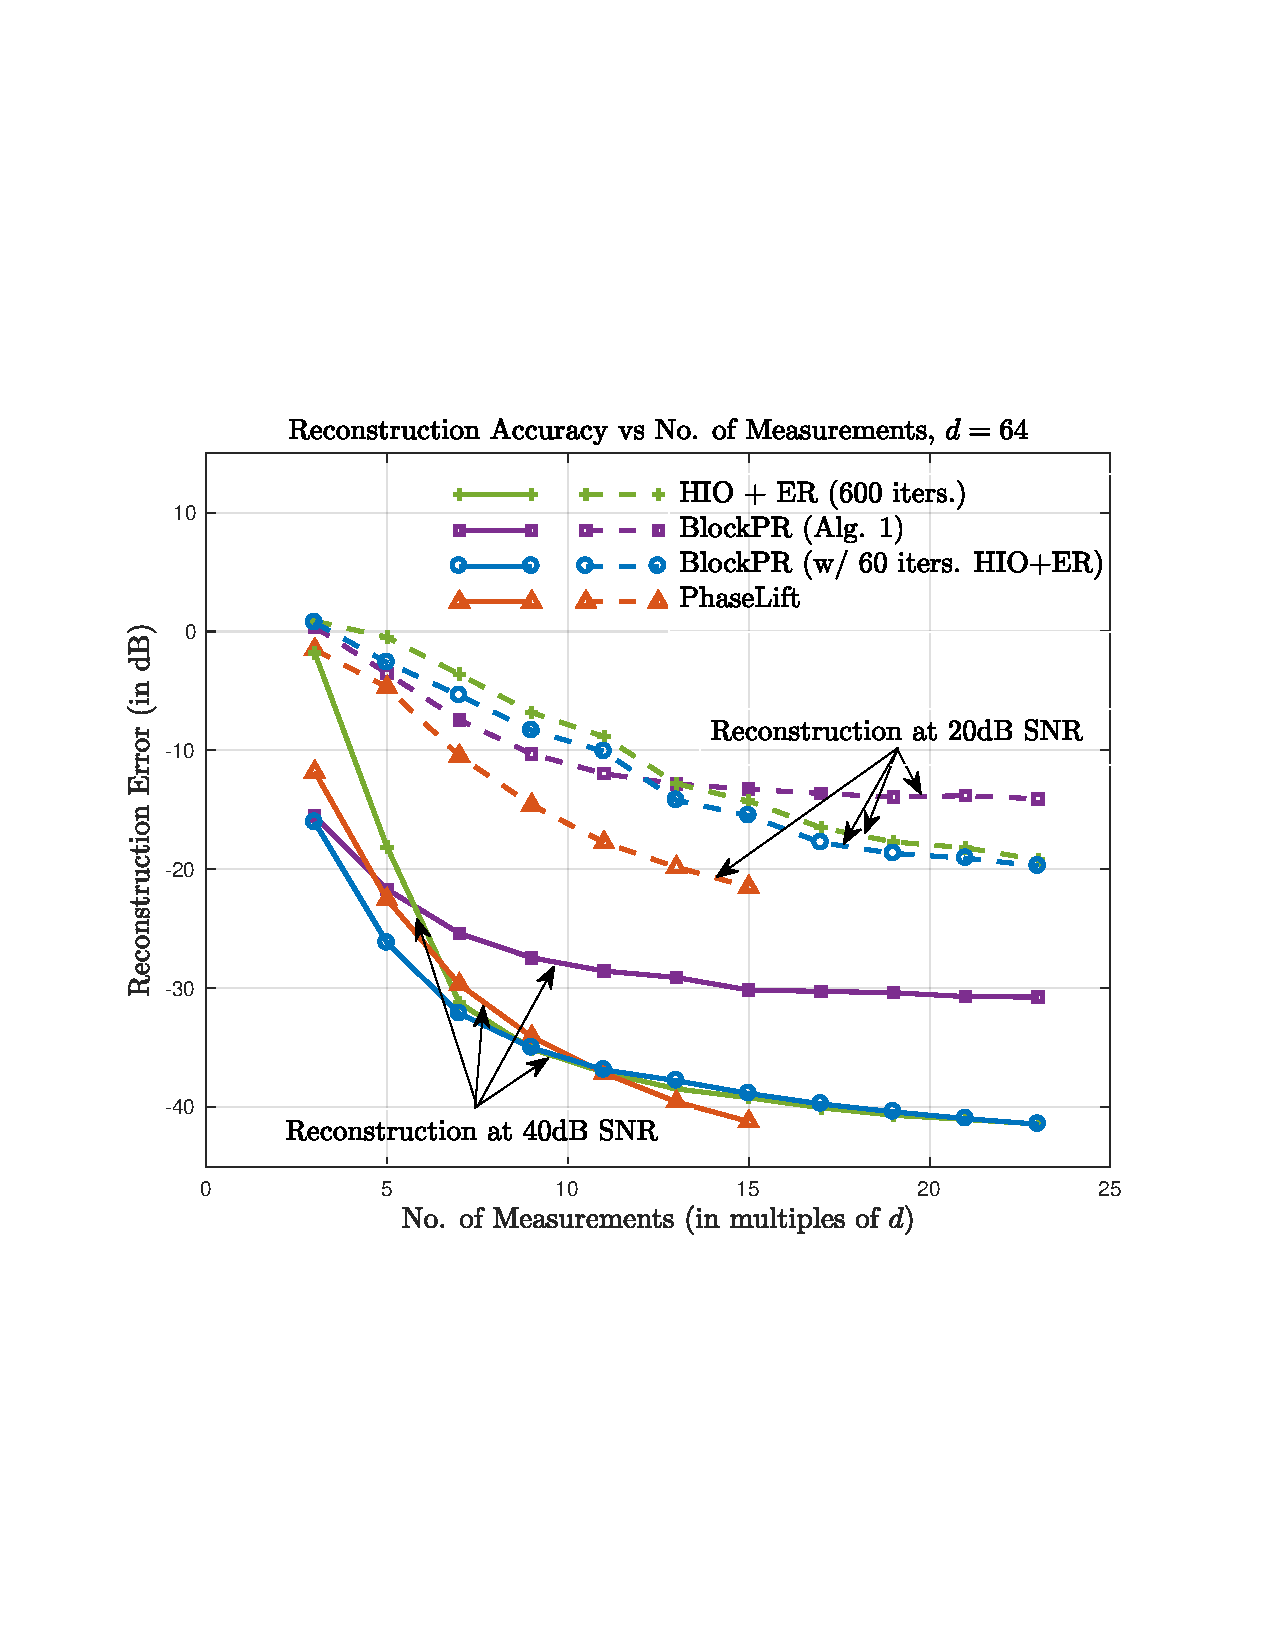
\includegraphics[clip=true, trim = 0.5in 2.5in 0.75in 2.5in,scale=0.45]{pics/fig5a}
%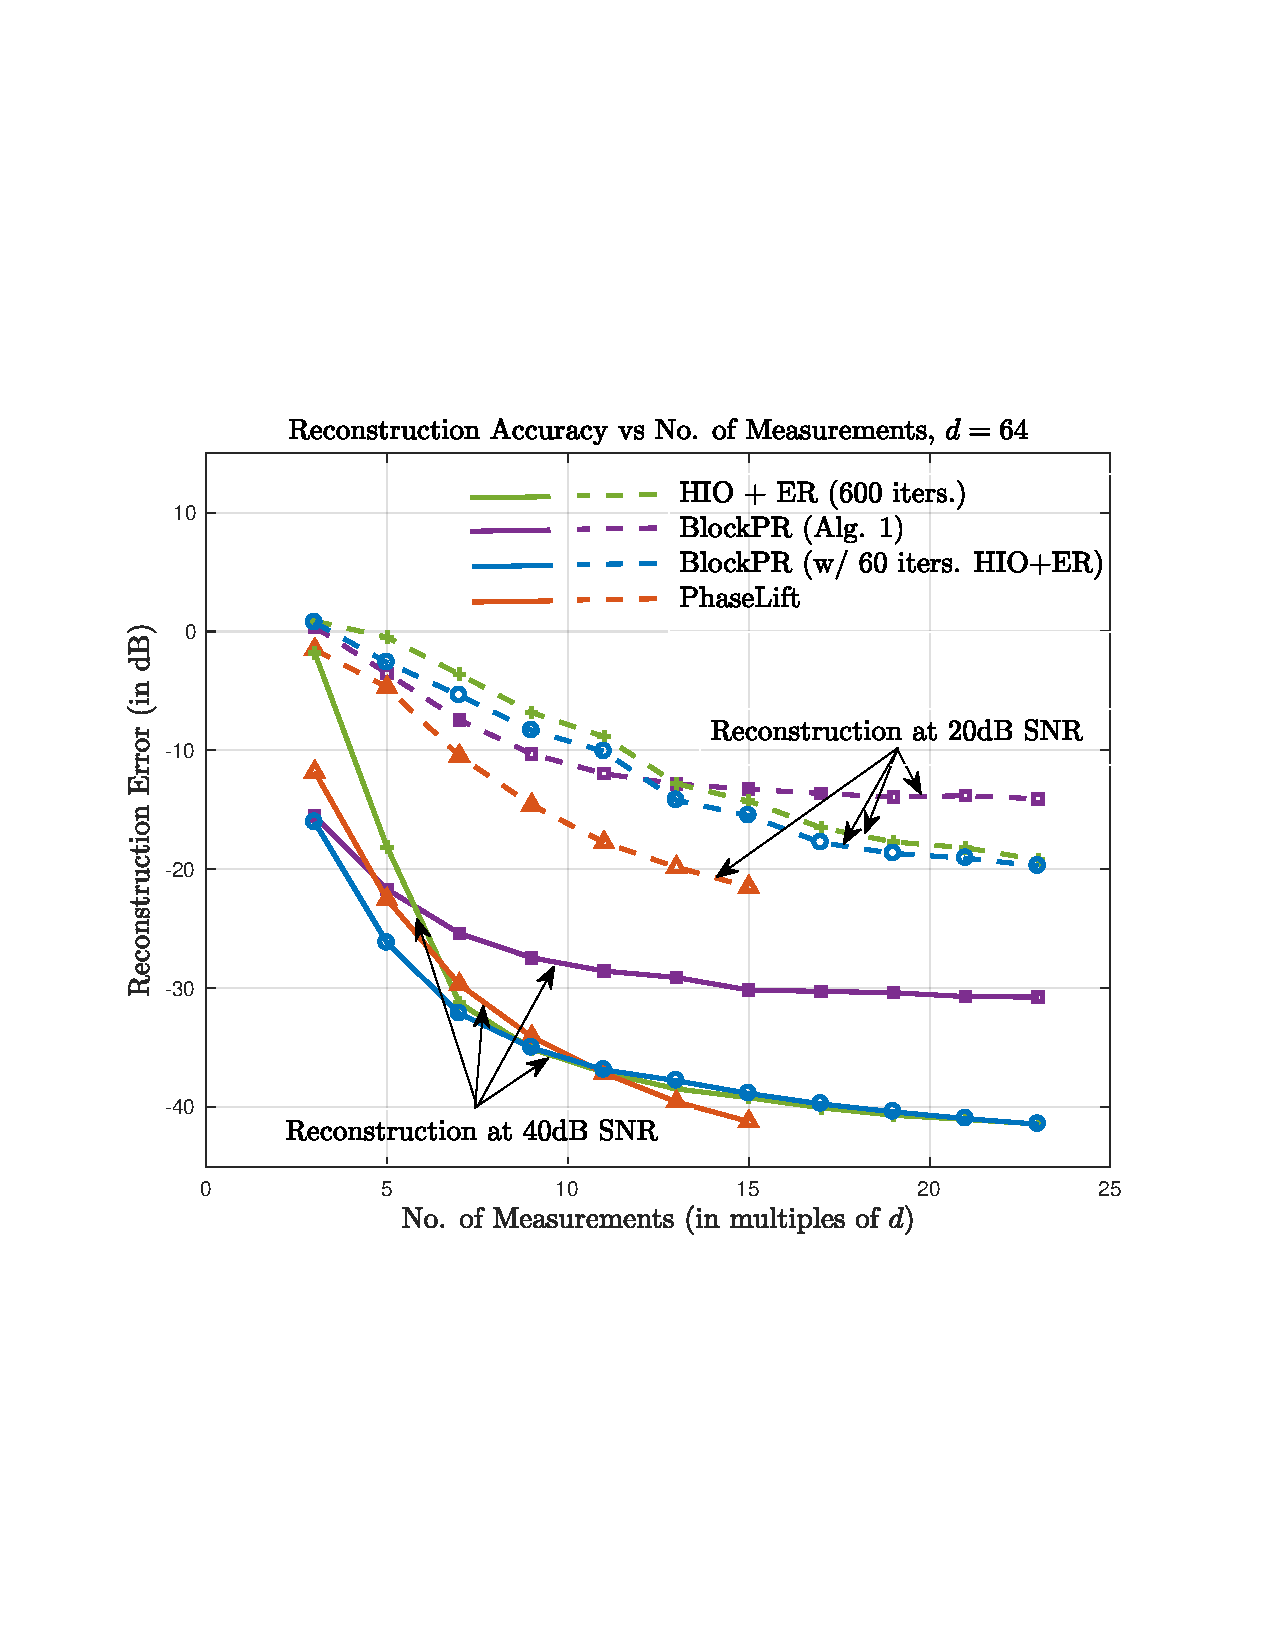
\includegraphics[clip=true, trim = 0.5in 2.5in 0.75in 2.5in,scale=0.42]{pics/measurements_600}
\caption{Reconstruction Error vs. No. of Measurements}
\label{fig:measurements}
\end{subfigure}
\hfill
\begin{subfigure}[b]{0.495\textwidth}
\centering
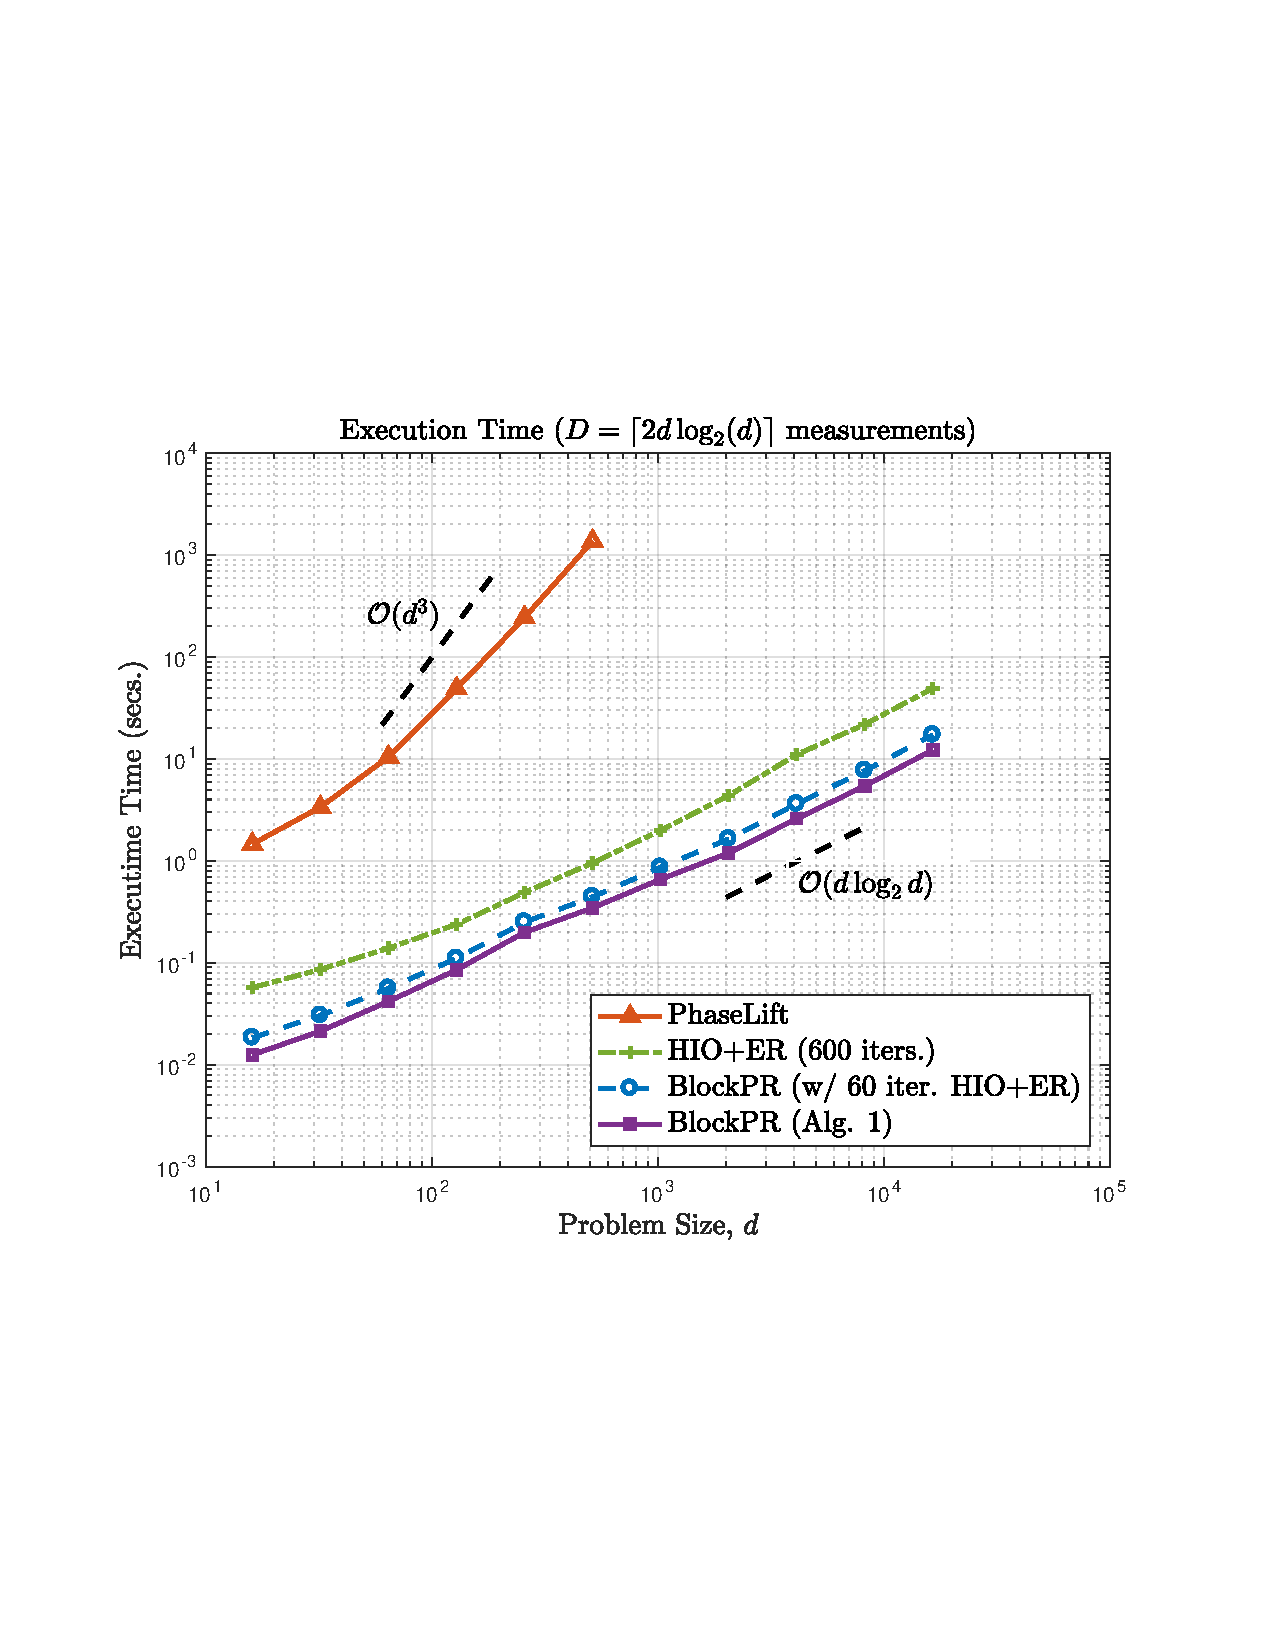
\includegraphics[clip=true, trim = 0.5in 2.5in 0.75in 2.5in,scale=0.45]{pics/fig5b}
\caption{Execution Time vs. Problem Size}
\label{fig:exectime}
\end{subfigure}
\caption{Performance Evaluation and Comparison of the Proposed Phase Retrieval Method 
(with Deterministic Local Correlation Measurements of Example 2, \S \ref{sec:MeasMatrix} and Additive Gaussian Noise)}
\label{fig:performance}
\end{figure}
%

Next, Fig. \ref{fig:measurements} plots the reconstruction error in recovering a $d=64$-length
complex vector as a function of the number of measurements used. This corresponds to using values of
$\delta$ ranging from $2$ to $12$ (and the associated $2\delta-1$ masks). As with Fig.
\ref{fig:noise-local}, the deterministic correlation-based measurement constructions of Section
\ref{sec:MeasMatrix} (Example construction $2$) were utilized along with an additive Gaussian noise
model. Plots are provided for simulations at two noise levels -- $20$ dB and $40$ dB. 
%For simplicity of visualization, we only plot results for the HIO alternating projection algorithm,
%{\em PhaseLift} and the two variants of the proposed algorithm (Alg. 1 and Alg. 1 w/ improved
%magnitude estimation and ER post-processing). 
Comparing the performance of the two {\em BlockPR} variants, we observe that the HIO+ER post-processing 
procedure provides improved reconstruction errors -- with the margin of improvement increasing when 
more measurements are available. We also notice that both variants of {\em BlockPR} compare
particularly well with the other algorithms (HIO+ER and {\em PhaseLift}) when small numbers of measurements are available.
%Additionally, when the improved magnitude estimation procedure is utilized, the proposed method is almost as
%accurate as the significantly more expensive {\em PhaseLift} algorithm and outperforms the popular 
%HIO algorithm by sometimes significant margins. 
%At the $40$ dB (moderate) noise 
%level, the proposed method provides the best reconstruction accuracy when approximately $7d$ or
%fewer measurements are available. 

Finally, Fig. \ref{fig:exectime} plots the average execution time (in seconds) required to solve the
phase retrieval problem using $D = \lceil 2d\log_2d\rceil$ measurements. For comparison, execution
times for the {\em PhaseLift} and HIO+ER alternating projection algorithms are provided. We observe
that both variants of the proposed method are several orders of magnitude faster than the {\em
PhaseLift} algorithm,\footnote{\ For computational efficiency and due to memory constraints, the {\em
PhaseLift} plot in Fig. \ref{fig:exectime} was generated using the TFOCS software package
(http://cvxr.com/tfocs/) instead of the more computationally expensive CVX software package.} and between
$2$--$5$ times faster than the HIO+ER implementation. Moreover, the plot illustrates the essentially
FFT-time computational complexity (see \S \ref{sec:RuntimeAlg1}) of the proposed method. Between the
two {\em BlockPR} variants, we see that there is a small trade-off between reduced execution time and
improved accuracy; one of the two variants may be more appropriate depending on the application
requirements.

\subsection{Experiments with Ptychographic Measurements from Example 1 of \S \ref{sec:MeasMatrix}}
\label{sec:PtychographicMeasExper}

%
\begin{figure}[hbtp]
\centering
\begin{subfigure}[b]{0.495\textwidth}
\centering
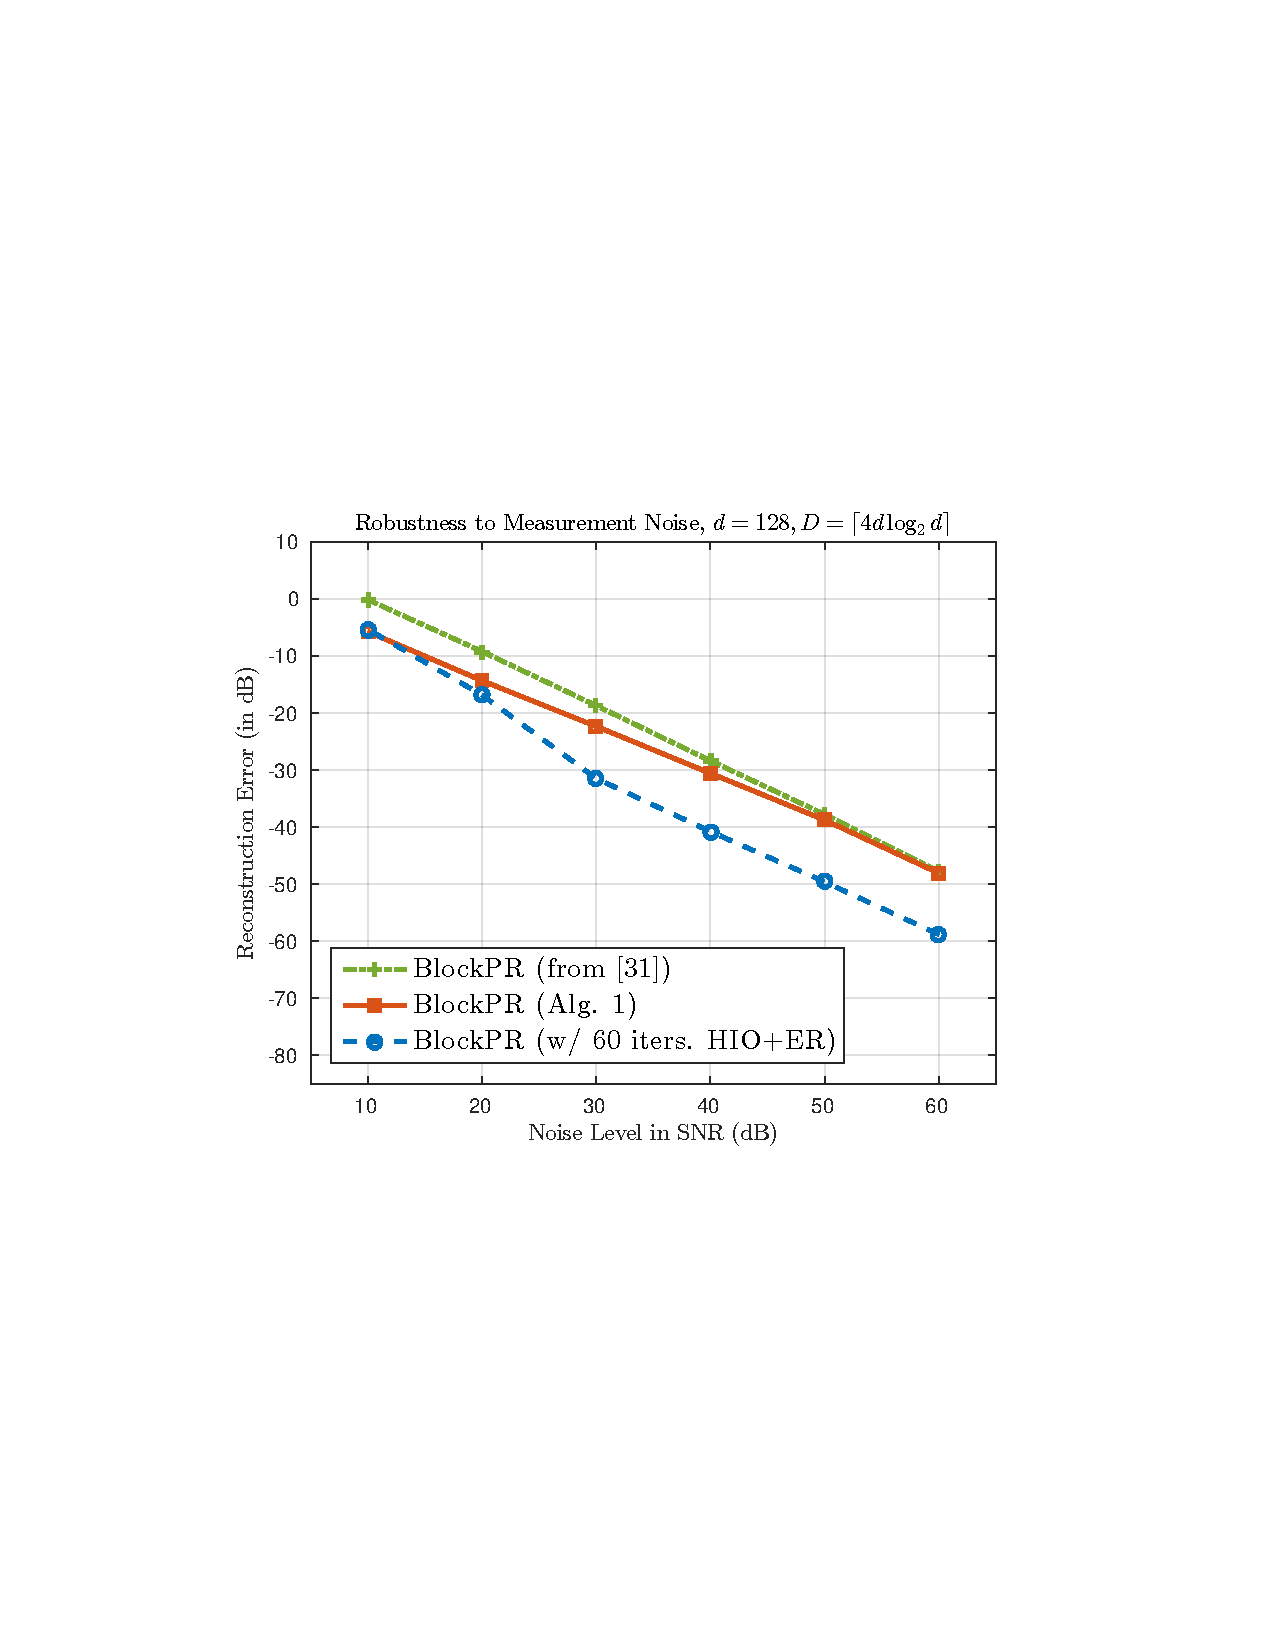
\includegraphics[clip=true, trim = 1.5in 3.35in 1.25in 3.25in,scale=0.59]{pics/fig6a}
\caption{Improved Robustness to Measurement Noise -- Comparing Variants of the {\em BlockPR}
algorithm}
\label{fig:global_vs_local_ptych}
\end{subfigure}
\hfill
\begin{subfigure}[b]{0.495\textwidth}
\centering
%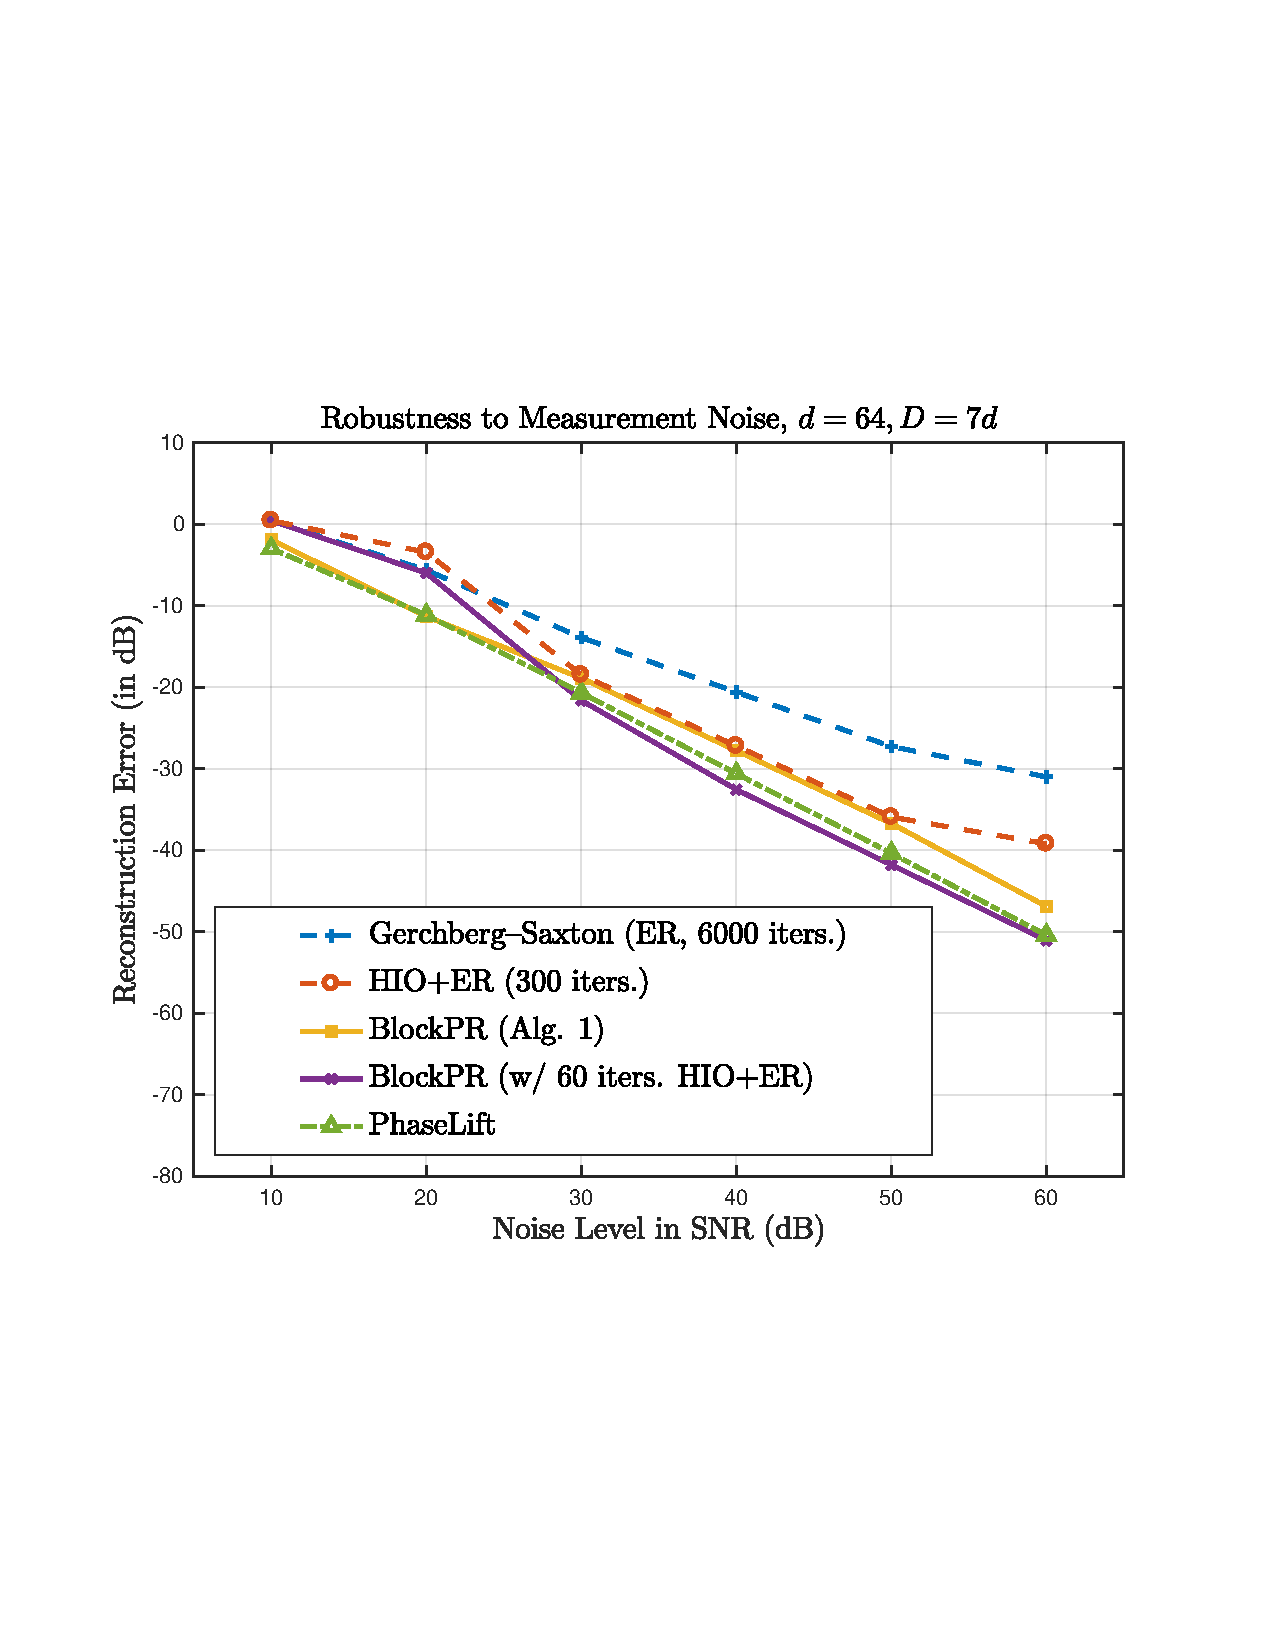
\includegraphics[clip=true, trim = 0.75in 2.75in 1in 2.5in,scale=0.45]{pics/fig6b}
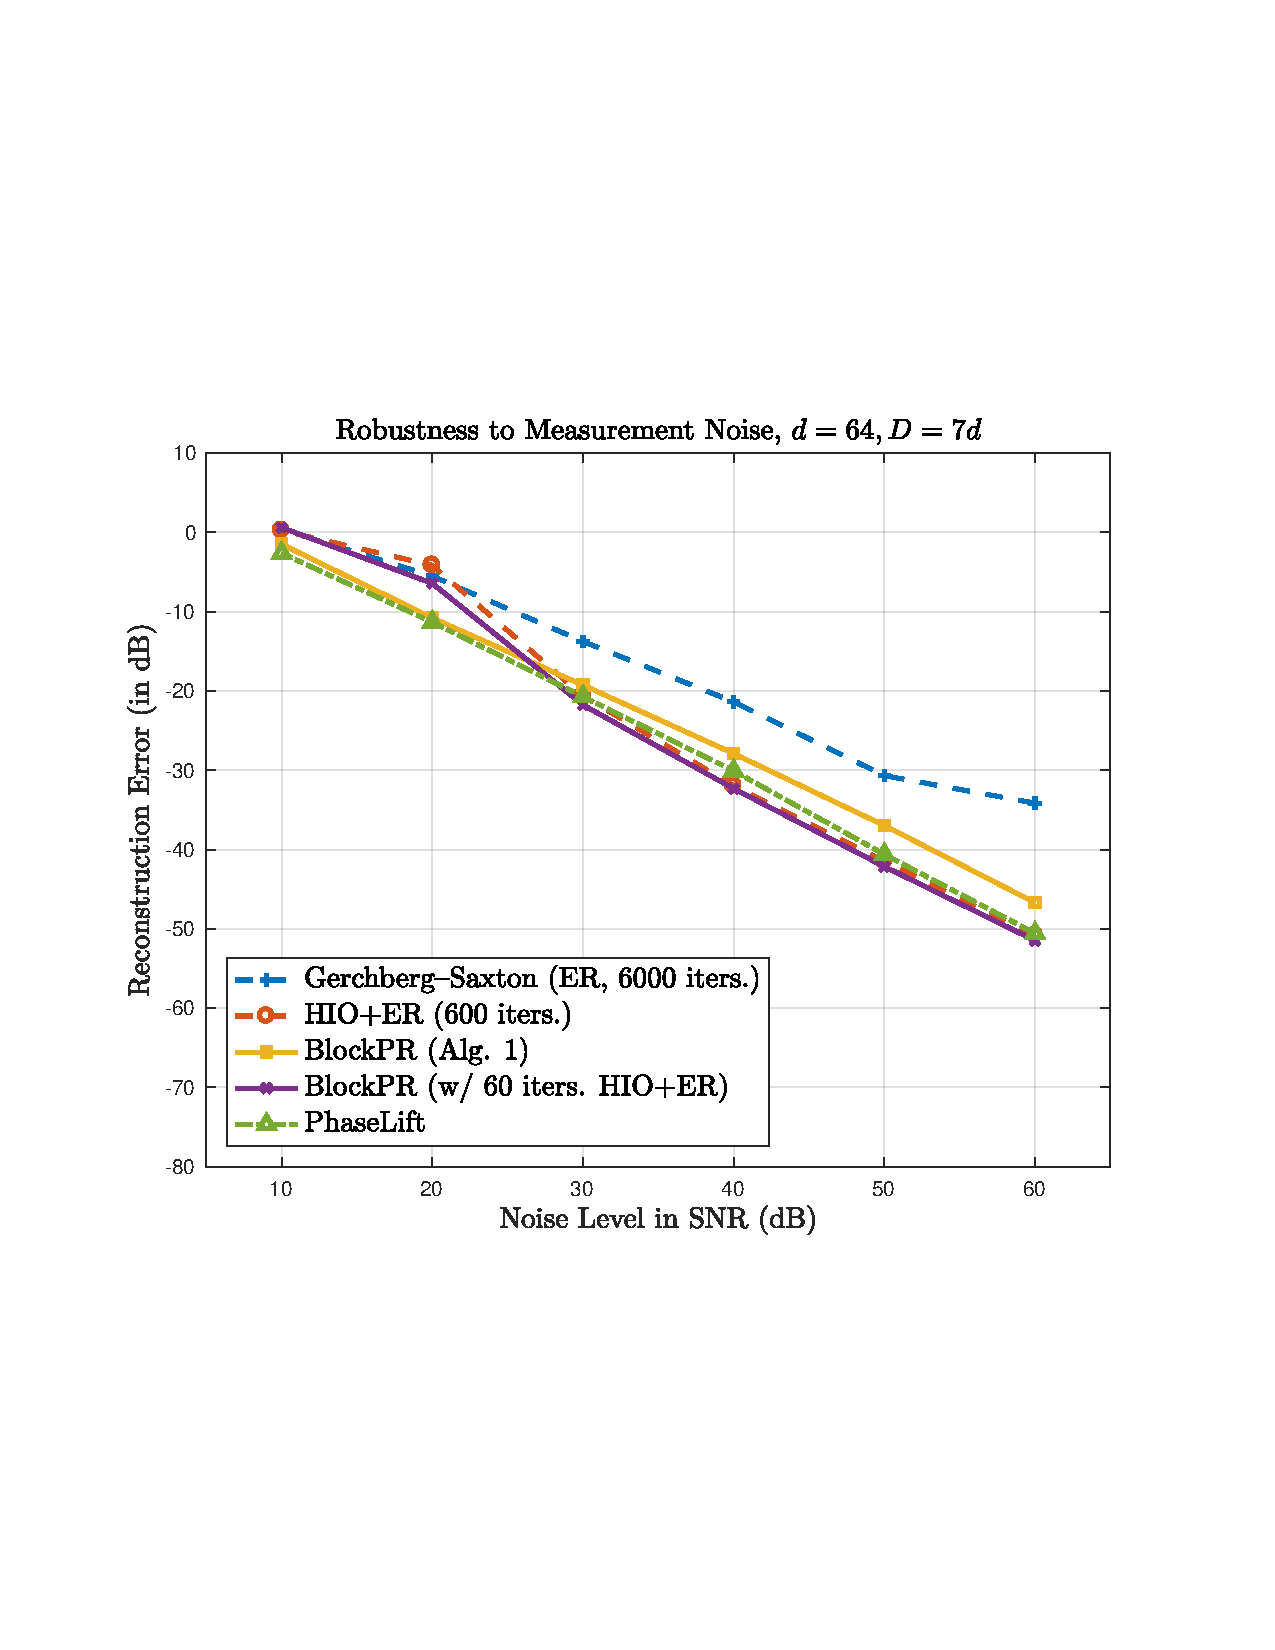
\includegraphics[clip=true, trim = 0.75in 2.75in 1in 2.5in,scale=0.45]{pics/robustness600_Fourier}
\caption{Phase Retrieval from $D=7d$ Measurements -- Comparison with Other Phase Retrieval Algorithms}
\label{fig:noise_robust_ptych}
\end{subfigure}
\caption{Numerical Evaluation of the Proposed Algorithm with the Ptychographic Measurements from
    Example 1 of \S \ref{sec:MeasMatrix}}
\label{fig:ptych_meas}
\end{figure}
%
%We now present a selection of empirical results demonstrating the accuracy, robustness and
%efficiency of the proposed method when using the ptychographic measurements from Example 1, \S
%\ref{sec:MeasMatrix}, while also noting that the qualitative and quantitative nature of the other
%results are similar to those presented in \S \ref{sec:SparseMeasureMasks}.  
{ We now present a selection of empirical results demonstrating the accuracy, robustness, and efficiency of the proposed method when using the ptychographic measurements from Example 1, \S\ref{sec:MeasMatrix} and observe that, in this case, the comparison between the proposed algorithm and existing methods is similar to that in section \S\ref{sec:SparseMeasureMasks}.}  Recall that (see Example 1 from \S \ref{sec:MeasMatrix} and \S \ref{sec:conn_pty} for details) this measurement construction
corresponds to a discretization of the ptychographic measurements $\left|\mathcal{F}[\widetilde h
\cdot S_l f](\omega) \right|^2$ as per \eqref{eq:ptych}, where $f$ is the unknown specimen and
$\widetilde h(t) = \frac{e^{-t/a}}{\sqrt[4]{2\delta -1}}$ denotes the {\em single, deterministic}
illumination function (or mask). As before, $\delta$ defines the local support of the illumination
function and we consider a discretization involving $2\delta-1$ Fourier modes and sample/specimen
shifts of $1$ unit or pixel (yielding a total of $d$ shifts in the discrete problem formulation). 

We begin with Fig. \ref{fig:global_vs_local_ptych}, which demonstrates the relative performance of
the {\em BlockPR} variants described in \cite{IVW2015_FastPhase} and this paper. More specifically,
we plot the error in reconstructing a $d=128$ length complex Gaussian test signal using $D = \lceil
4d\log_2 d\rceil$ measurements at different added noise levels. As with Fig.
\ref{fig:eig_vs_greedy}, we plot results for three different variants of the {\em BlockPR}
algorithm: (i) Algorithm \ref{alg:phaseRetrieval1}, (ii) Algorithm \ref{alg:phaseRetrieval1} with
the HIO+ER post-processing procedure as described in \S \ref{sec:SparseMeasureMasks}, and (iii) the implementation
from \cite{IVW2015_FastPhase}. We again observe (as in Fig. \ref{fig:eig_vs_greedy}) that the methods
described in this paper (which use eigenvector-based angular synchronization) are more accurate than
that detailed in \cite{IVW2015_FastPhase} (which uses a greedy angular synchronization method), with
the improvement in performance being especially significant at low SNRs. Next, Fig.
\ref{fig:noise_robust_ptych} studies the performance of the proposed method(s) against three other
popular phase retrieval algorithms -- {\em PhaseLift}, the {\em Gerchberg--Saxton} Error Reduction
(ER) algorithm, and the Hybrid Input--Output (HIO) algorithm (with implementation parameters identical to those in 
\S \ref{sec:SparseMeasureMasks}). As with Fig. \ref{fig:noise-7d}, we
consider the reconstruction of a $d = 64$ length complex vector $x_0$ using $D = 7d$ measurements in
the presence of additive Gaussian noise. We observe that the methods proposed in this paper outperform the 
ER algorithm and compare very well with the HIO+ER and (the significantly more expensive) {\em PhaseLift} 
algorithms across a wide range of SNRs. 
%While there may be an optimal set of
%algorithmic parameters which improve the convergence of the ER and HIO algorithms, the selection of
%such parameters is not immediately obvious. 
Finally, we note that the execution time plot for this
ptychographic measurement construction is qualitatively and quantitatively similar to Fig.
\ref{fig:exectime} -- the proposed methods are faster (by a factor of $2$--$5$) than an equivalent HIO+ER
implementation and orders of magnitude faster than convex optimization approaches such as {\em
PhaseLift}. 

%Moreover, the interested reader is
%encouraged to download the open source code implementing these results at \cite{bitbucket_BlockPR}
%and run their own experiments. \textcolor{red}{add exec time plot or just say it is the same as in
%Fig. 4b?} Finally, we plot the execution time
%-- NOTE:  HIO and ER as convex opt. ref. -- -- A reformulation of ER and HIO as convex optimization methods, probably worth a closer read -- also justifies Aditya's HIO implementation \cite{bauschke2002phase}\\


\section{Concluding Remarks}
\label{sec:conclusion}

In this paper new and improved deterministic robust recovery guarantees are proven for the phase retrieval problem using local correlation measurements.  In addition, a new practical phase retrieval algorithm is presented which is both faster and more noise robust than previously existing approaches (e.g., alternating projections) for such local measurements.  

Future work might include the exploration of more general classes of measurements which are guaranteed to lead to well conditioned linear systems  of the type used to reconstruct $X \approx X_0$ in line 1 of Algorithm~\ref{alg:phaseRetrieval1}.  Currently two deterministic measurement constructions are known (recall, e.g., Section~\ref{sec:MeasMatrix}) -- it should certainly be possible to construct more general families of such measurements.

Other interesting avenues of inquiry include the theoretical analysis of the magnitude estimate approach proposed in Section~\ref{sec:MagEstImpNumerical} in combination with the rest of Algorithm~\ref{alg:phaseRetrieval1}.  Alternate phase retrieval approaches might also be developed by using such local block eigenvector-based methods for estimating phases too, instead of just using the single global top eigenvector as currently done in line 3 of Algorithm~\ref{alg:phaseRetrieval1}.

Finally, more specific analysis of the performance of the proposed methods using masked/windowed Fourier measurements (recall Section~\ref{sec:STFT}) would also be interesting.  In particular, an analysis of the performance of such approaches as a function of the bandwidth of the measurement mask/window could be particularly enlightening.  One might also consider extending the discrete results of this paper to the analytic setting by, e.g., expanding on \cite{merhi2017recovery}.   

\bibliographystyle{abbrv}
\bibliography{SparsePR}

\appendix

%%%%%%%%%%%%%%%%%%%%%%%%%%%%%%%%%%%%%%%%%%%%%%%%%%%%%%%
\section{Alternate Perturbation Bounds}
\label{sec:AltPerturbBounds}
In this section we present a simpler (and easier to derive), albeit weaker,  perturbation result in the spirit of Section \ref{sec:Perturb}, which is associated with the analysis of line 3 of Algorithm~\ref{alg:phaseRetrieval1}.
%\subsection{General Perturbation Results}
Specifically, we will derive an upper bound on $\min_{\theta\in[0,2\pi]} \Vert \tx_0 - \mathbbm{e}^{\mathbbm{i}\theta}\tx \Vert_2$ (provided by Theorem~\ref{cor2:GenBound}), which scales like $d^3$.  While this dependence is strictly worse than the one derived in Section \ref{sec:Perturb}, it is easier to obtain and the technique may be of independent interest. 

We will begin with a result concerning the top eigenvector of any Hermitian matrix.  %Note that the bound we obtain depends only on the spectral gap of the unperturbed matrix $\X_0$, as opposed to the type of bound obtained via a straightforward application of, e.g., the $\sin \theta$ theorem \cite{davis1970rotation,stewart1990matrix}.

\begin{lem}
Let $\X_0 = \sum^d_{j=1} \nu_j \x_j\x_j^*$ be Hermitian with eigenvalues $\nu_1 \geq \nu_2 \geq \dots \geq \nu_d$ and orthonormal eigenvectors $\x_1, \dots, \x_d \in \mathbbm{C}^d$.  Suppose that $\X = \sum^d_{j=1} \lambda_j \v_j\v_j^*$ is Hermitian with eigenvalues $\lambda_1 \geq \lambda_2 \geq \dots \geq \lambda_d$, orthonormal eigenvectors $\v_1, \dots, \v_d \in \mathbbm{C}^d$, and $\Vert \X-\X_0 \Vert_{\rm F}~\leq \eta \Vert \X_0 \Vert_F$ for some $\eta \geq 0$.  Then, %there exists a $\theta \in [0, 2 \pi]$ such that
\[ \left( 1 - | \langle \x_1, \v_1 \rangle |^2 \right)  \leq  \frac{4 \eta^2 \Vert \X_0 \Vert^2_{\rm F} }{(\nu_1- \nu_2)^2} .\]
%whenever $2\eta \Vert \X_0 \Vert_F \leq |\nu_1 - \nu_2|$.  
%%If $\lambda_2 = \nu_2$ always holds (as per \S\ref{sec:Spectrum} with $\X_0 = \tilde{\X}_0$ and $\X = \tilde{\X}$) then \[ \left( 1 - | \langle \x_1, \v_1 \rangle |^2 \right)  \leq  \frac{\eta^2 \Vert \X_0 \Vert^2_{\rm F} }{(\nu_1- \nu_2)^2}. \]
%%will hold for all $\eta \geq 0$.
        \label{lem:GenBound}
\end{lem}

\begin{proof}
An application of the $\sin \theta$ theorem \cite{davis1970rotation,stewart1990matrix} (see, e.g., the proof of Corollary 1 in \cite{yu2015useful}) tells us that 
\begin{equation*}
\sin \left( \arccos \left( | \langle \x_1, \v_1 \rangle | \right) \right) \leq \frac{2 \eta \Vert \X_0 \Vert_F}{|\nu_1 - \nu_2|}.
%\label{equ:SinthetaApp}
\end{equation*}
Squaring both sides we then learn that 
\begin{equation}
 \left( 1 - | \langle \x_1, \v_1 \rangle |^2 \right)  = \sin^2 \left( \arccos \left( | \langle \x_1, \v_1 \rangle | \right) \right) \leq \frac{4 \eta^2 \Vert \X_0 \Vert^2_F}{(\nu_1 - \nu_2)^2},
%\label{equ:SinthetaApp}
\end{equation}
%%Considering the denominator, we can see that 
%%$$|\nu_1 - \lambda_2| \geq |\nu_1 - \nu_2| - |\nu_2 - \lambda_2| \geq |\nu_1 - \nu_2| -  \eta \Vert \X_0 \Vert_F$$
%%by Weyl's inequality (see, e.g., \cite{horn2012matrix}).  Thus, $|\nu_1 - \lambda_2| \geq \frac{|\nu_1 - \nu_2|}{2}$ whenever $2\eta \Vert \X_0 \Vert_F \leq |\nu_1 - \nu_2|$
giving us the desired inequality.  
%%For the second inequality we simply use $\lambda_2 = \nu_2$ in \eqref{equ:SinthetaApp}.
\end{proof}

The following variant of Lemma~\ref{lem:GenBound} concerning rank 1 matrices $\X_0$ is of use in the analysis of many other phase retrieval methods, and can be used, e.g., to correct and simplify the proof of equation (1.8) in Theorem 1.3 of \cite{candes2014solving}.

\begin{lem}
Let $\x_0 \in \mathbb C^d$, set $\X_0 = \x_0\x_0^*$, and let 
$\X \in \mathbb C^{d \times d}$ be Hermitian with $\Vert \X~-~\X_0 \Vert_F~\leq \eta
\Vert \X_0 \Vert_F = \eta \Vert \x_0\Vert_2^2$ for some $\eta \geq 0$.  Furthermore, let $\lambda_i$ be the $i$-th largest magnitude
eigenvalue of $\X$ and $\v_i \in \mathbb{C}^d$ an associated eigenvector, such 
that the $\v_i$ form an orthonormal eigenbasis. Then
\[ \min_{\theta \in [0, 2 \pi]} \Vert  \mathbbm{e}^{\mathbbm{i} \theta}  \x_0 - \sqrt{ 
    |\lambda_1 |} \v_1 \Vert_2 \leq (1+2 \sqrt{2}) \eta \Vert \x_0 
        \Vert_2.\footnote{It is interesting to note that similar bounds can also be obtained using simpler techniques (see, e.g., \cite{CandesFix}).} \]
        \label{cor:rank1Bound}
\end{lem}

\begin{proof}
In this special case of Lemma~\ref{lem:GenBound} we have $\nu_1 = \Vert \X_0 \Vert_F = \Vert \x_0\Vert_2^2$ and $\x_1 := \x_0 / \Vert \x_0 \Vert$.  Choose $\phi \in [0, 2 \pi]$ such that $\langle \mathbbm{e}^{\mathbbm{i} \phi} \x_0, \v_1 \rangle  = \vert \langle  \x_0, \v_1 \rangle \vert$.  Then, 
%
\begin{align}
 \Vert \mathbbm{e}^{\mathbbm{i} \phi} \x_0 - \sqrt{\nu_1} \v_1 \Vert_2^2 &= 2\nu_1 - 2 \nu_1  \cdot \vert \langle  \x_0 / \Vert \x_0 \Vert, \v_1 \rangle \vert = 2\nu_1 - 2 \nu_1  \cdot \vert \langle  \x_1, \v_1 \rangle \vert \nonumber \\ &\leq 2 \nu_1 \left( 1 - \vert \langle  \x_1, \v_1 \rangle \vert \right) \left( 1 + \vert \langle  \x_1, \v_1 \rangle \vert \right) \label{equ:CorIntermed} \\ &= 2 \nu_1 \left( 1 - | \langle \x_1, \v_1 \rangle |^2 \right) \leq 8 \eta^2 \Vert \X_0 \Vert_{\rm F} \nonumber
\end{align}
where the last inequality follows from Lemma~\ref{lem:GenBound} with $\nu_1 = \Vert \X_0 \Vert_F = \Vert \x_0\Vert_2^2$.  Finally, by the triangle inequality, Weyl's inequality (see, e.g., \cite{horn2012matrix}), and \eqref{equ:CorIntermed}, we have
\begin{align*}
  \Vert \mathbbm{e}^{\mathbbm{i} \phi} \x_0 - \sqrt{ |\lambda_1|} \v_1 \Vert_2 & \leq \Vert 
    \mathbbm{e}^{\mathbbm{i} \phi} \x_0 -\sqrt \nu_1 \v_1 \Vert_2 + \Vert \sqrt \nu_1 \v_1 - 
    \sqrt{|\lambda_1|} \v_1 \Vert_2 \\
    & \leq 2 \sqrt{2} \cdot \eta \sqrt \nu_1 + \left \vert \sqrt \nu_1 - \sqrt{|\lambda_1|} \right \vert \\ & \leq 2 \sqrt{2} \cdot \eta \sqrt 
        \nu_1 + \frac{| \nu_1 - \lambda_1 |}{\sqrt \nu_1 + \sqrt{|\lambda_1|}} \\
     & \leq 2 \sqrt{2} \cdot \eta \sqrt \nu_1 + \frac{\eta \nu_1}{\sqrt \nu_1 + \sqrt{|\lambda_1|}}\\ 
    & \leq (1+2 \sqrt{2}) \eta \sqrt \nu_1.
\end{align*}
The desired result now follows.
\end{proof}

We may now use Lemma~\ref{lem:GenBound} to produce a perturbation bound for our banded matrix of phase differences $\tilde{\X}_0$ from \eqref{eq:X_0}.

\begin{theorem}
Let $\tX_0 = T_{\delta}(\tx_0 \tx_0^*)$ where $|(\tx_0)_i| = 1$ for each $i$.  Further suppose $\tX \in T_{\delta}(\H^d)$ has $\tx$ as its top eigenvector, where $||\tx||_2 = \sqrt{d}$.  Suppose that $\Vert \tX_0 - \tX \Vert_F \le \eta \Vert \tX_0 \Vert_F$ 
%Let $\tilde{\X}_0$ be the Hermitian matrix from \eqref{equ:MatrixofPhases} with eigenvalues $\lambda_1 = 2 \delta - 1 \geq \ldots \ge \lambda_d$, and $\| \tilde{\X}_0 \|^2_{\rm F} = d (2 \delta - 1)$.  Let $\tilde{\X}$ be the Hermitian matrix from line 4 of Algorithm~\ref{alg:phaseRetrieval}, and suppose that $\Vert \tilde{\X} - \tilde{\X}_0 \Vert_{\rm F}~\leq \eta \Vert \tilde{\X}_0 \Vert_F$ 
for some $\eta>0$.  Then, there exists an absolute constant $C \in \mathbb{R}^+$ such that
%\[ \left( 1 - \frac{1}{d^2}| \langle \tilde{\x}_0, \tilde{\x} \rangle |^2 \right)  \leq  C \eta^2 \left( \frac{d}{\delta} \right)^5 \]
%        \label{cor2:GenBound}
%where the phase vectors $\tilde{\x}$ and $\tilde{\x}_0$ are normalized such that $\| \tilde{\x} \|_2 = \| \tilde{\x}_0 \|_2 = \sqrt{d}$.
\[\min_{\theta\in[0,2\pi]} \Vert \tx_0 - \mathbbm{e}^{\mathbbm{i}\theta} \tx \Vert_2 \le C\bigfrac{\eta d^3}{\delta^{\frac{5}{2}}}.\]

\label{cor2:GenBound}
\end{theorem}

\begin{proof}
Recall that the phase vectors $\tilde{\x}$ and $\tilde{\x}_0$ are normalized so that $\| \tilde{\x} \|_2 = \| \tilde{\x}_0 \|_2 = \sqrt{d}$.  Combining Lemmas~\ref{lem:EigGap} and \ref{lem:GenBound} after noting that $\| \tilde{\X}_0 \|^2_{\rm F} = d (2 \delta - 1)$ we learn that 
\begin{equation}
\left( 1 - \frac{1}{d^2}| \langle \tilde{\x}_0, \tilde{\x} \rangle |^2 \right)  \leq  C' \eta^2 \left( \frac{d}{\delta} \right)^5
\label{equ:cor2GenBIP}
\end{equation}
for an absolute constant $C' \in \mathbb{R}^+$.  Let $\phi \in [0,2 \pi)$ be such that $\operatorname{Re}\left( \langle \tilde{\x}_0,\mathbbm{e}^{\mathbbm{i} \phi} \tilde{\x} \rangle \right) = \left| \langle \tilde{\x}_0, \tilde{\x} \rangle \right|$.  Then,
\begin{align*}
\| \tilde{\x}_0 - \mathbbm{e}^{\mathbbm{i} \phi} \tilde{\x} \|^2_2 &= 2d - 2 \operatorname{Re}\left( \langle \tilde{\x}_0,\mathbbm{e}^{\mathbbm{i} \phi} \tilde{\x} \rangle \right) \\
&= 2d \left( 1 - \frac{1}{d} \left| \langle \tilde{\x}_0, \tilde{\x} \rangle \right| \right) \leq 2d \left( 1 - \frac{1}{d^2} \left| \langle \tilde{\x}_0, \tilde{\x} \rangle \right|^2 \right).
\end{align*}
Combining this last inequality with \eqref{equ:cor2GenBIP} concludes the proof.
\end{proof}

%%%\begin{lem}
%%%Let $\X_0 = \sum^d_{j=1} \nu_j \x_j\x_j^*$ be Hermitian with eigenvalues $\nu_1 \geq |\nu_2| \geq \dots \geq |\nu_d|$, $\nu_1 > 0$, and orthonormal eigenvectors $\x_1, \dots, \x_d \in \mathbbm{C}^d$.  Suppose that $\X = \sum^d_{j=1} \lambda_j \v_j\v_j^*$ is Hermitian with eigenvalues $|\lambda_1| \geq |\lambda_2| \geq \dots \geq |\lambda_d|$, orthonormal eigenvectors $\v_1, \dots, \v_d \in \mathbbm{C}^d$, and $\Vert \X-\X_0 \Vert_{\rm F}~\leq \eta \Vert \X_0 \Vert_F$ for some $\eta>0$.  Then, %there exists a $\theta \in [0, 2 \pi]$ such that
%%%\[ \left( 1 - | \langle \x_1, \v_1 \rangle |^2 \right)  \leq  \frac{3 \eta(\frac{3}{2} \eta +1 )\Vert \X_0 \Vert^2_{\rm F} }{\nu_1(\nu_1- |\nu_2|)} \]
%%%        \label{lem:GenBound}
%%%\end{lem}
%%%
%%%%Note that a straightforward application of the $\sin \theta$ theorem based on an arbitrary perturbation in the Frobenius norm as per Lemma~\ref{lem:GenBound} gives the bound 
%%%%$$\left( 1 - | \langle \x_1, \v_1 \rangle |^2 \right)  \leq \frac{\eta^2 \Vert \X_0 \Vert^2_{\rm F}}{(\nu_1- |\nu_2|)^2}.$$
%%%%Comparing this to the conclusion of Lemma~\ref{lem:GenBound}, we can see that Lemma~\ref{lem:GenBound} provides a better upper bound whenever $\eta > \frac{6(\nu_1- |\nu_2|)}{2\nu_1 - 9(\nu_1- |\nu_2|)}$.  
%%%
%%%\begin{proof}
%%%Consider that 
%%%\[\begin{array}{rcl}
%%%\sqrt{\sum_{j=2}^d \lambda_j^2} - \sqrt{\sum_{j=2}^d \nu_j^2} & \le & \sqrt{\sum_{j=2}^d(\lambda_j - \nu_j)^2} \\
%%%& \le & \sqrt{\sum_{j=1}^d(\lambda_j - \nu_j)^2} \\
%%%& \le & \eta||X_0||_{\rm F}, 
%%%\end{array}.\]
%%%where the first inequality comes from the triangle inequality and the last comes from the Wielandt-Hoffman inequality \cite{hoffman1953variation}.  This gives
%%%\[ \sqrt{\sum_{j=2}^d \lambda_j^2} \le \sqrt{\sum_{j=2}^d \nu_j^2} + \eta ||X_0||_{\rm F}.\]
%%%
%%%% Let $V \in \mathbbm{C}^{d \times d}$ be the unitary matrix with $v_j$ as its $j^{\rm th}$ column, and let $\Lambda \in \mathbbm{R}^{d \times d}$ be a diagonal matrix whose $j^{\rm th}$ diagonal entry is $\lambda_j$.  We have that
%%%% \begin{align*}
%%%%  \sqrt{\sum^d_{j=2} \lambda^2_j }&\leq \sqrt{2 \lambda^2_1 + \sum^d_{j = 2} \lambda^2_j - 2 \lambda_1 \sum^d_{j=1} \lambda_j \left| \left(  V^* \x_1 \right)_j \right|^2} \\ 
%%%%  &= \sqrt{\Vert \X \Vert^2_{\rm F} - 2 \lambda_1{\rm Trace} \left(\Lambda (V^* x_1)(V^* x_1)^* \right) + \lambda^2_1}\\ 
%%%%  &= \Vert \Lambda - \lambda_1 (V^* \x_1)(V^* \x_1)^* \Vert_{\rm F} \\
%%%%  &= \Vert \X - \lambda_1 \x_1 \x^*_1 \Vert_{\rm F} \\
%%%%  & \leq \Vert \X - \X_0 \Vert_{\rm F} +  \Vert \X_0 - \nu_1  \x_1 \x^*_1 \Vert_{\rm F} +  \Vert \nu_1  \x_1 \x^*_1 - \lambda_1 \x_1 \x^*_1 \Vert_{\rm F}\\
%%%%  &\leq 2 \eta \Vert \X_0 \Vert_{\rm F} + \sqrt{\sum^d_{j=2} \nu^2_j },
%%%%  \end{align*}
%%%% where the last inequality uses our assumption, and Weyl's inequality.  
%%%As a result, we have that
%%%\begin{align*}
%%% \Vert \X_0 - \nu_1 \v_1 \v^*_1 \Vert_{\rm F} &\leq  \Vert \X_0 - \X \Vert_{\rm F} + \Vert \X- \nu_1 \v_1 \v^*_1 \Vert_{\rm F} \\
%%% & \leq \eta \Vert \X_0 \Vert_{\rm F} + \left \Vert (\lambda_1- \nu_1 ) \v_1 \v^*_1 + \sum^d_{j=2} \lambda_j \v_j\v_j^* \right \Vert_{\rm F}\\
%%% & \leq 2 \eta \Vert \X_0 \Vert_{\rm F} +  \sqrt{\sum^d_{j=2} \lambda^2_j }
%%% \end{align*}
%%%using our assumption and Weyl's inequality (see, e.g., \cite{horn2012matrix}).  Finally, we may now use our previous bound to obtain
%%%\begin{equation}
%%%\Vert \X_0 - \nu_1 \v_1 \v^*_1 \Vert_{\rm F}  \leq 3 \eta \Vert \X_0 \Vert_{\rm F} + \sqrt{\sum^d_{j=2} \nu^2_j }.
%%%\label{equ:FrobBB}
%%%\end{equation}
%%%
%%%Expanding this last norm we obtain
%%%\begin{align*}
%%% \Vert \X_0 - \nu_1 \v_1 \v^*_1 \Vert^2_{\rm F} &=  \Vert \X_0 \Vert^2_{\rm F} - 2 \nu_1 {\rm Trace} \left(  \X^*_0 \v_1 \v^*_1\right) + \nu^2_1\\
%%% &= \sum^d_{j=1} \nu^2_j - 2 \nu_1 \sum_{j=1}^d \nu_j | \langle \x_j, \v_1 \rangle |^2 + \nu^2_1\\
%%% &= 2 \nu^2_1 \left( 1 - | \langle \x_1, \v_1 \rangle |^2 \right) + \sum^d_{j=2} \nu^2_j - 2 \nu_1 \sum_{j=2}^d \nu_j | \langle \x_j, \v_1 \rangle |^2.
%%%\end{align*}
%%%Thus, we have that
%%%\begin{align*}
%%%2 \nu^2_1 \left( 1 - | \langle \x_1, \v_1 \rangle |^2 \right) &=  \Vert \X_0 - \nu_1 \v_1 \v^*_1 \Vert^2_{\rm F} + 2 \nu_1 \sum_{j=2}^d \nu_j | \langle \x_j, \v_1 \rangle |^2 - \sum^d_{j=2} \nu^2_j \\
%%%&\leq \Vert \X_0 - \nu_1 \v_1 \v^*_1 \Vert^2_{\rm F} + 2 \nu_1 |\nu_2| \sum_{j=2}^d | \langle \x_j, \v_1 \rangle |^2 - \sum^d_{j=2} \nu^2_j \\
%%%&= \Vert \X_0 - \nu_1 \v_1 \v^*_1 \Vert^2_{\rm F} + 2 \nu_1 |\nu_2| \left( 1 - | \langle \x_1, \v_1 \rangle |^2 \right) - \sum^d_{j=2} \nu^2_j.
%%%\end{align*}
%%%Rearranging once more, we have that
%%%$$(2 \nu^2_1- 2 \nu_1 |\nu_2| ) \left( 1 - | \langle \x_1, \v_1 \rangle |^2 \right) \leq \Vert \X_0 - \nu_1 \v_1 \v^*_1 \Vert^2_{\rm F} - \sum^d_{j=2} \nu^2_j.$$
%%%Using $\eqref{equ:FrobBB}$ now gives us that
%%%\begin{align}
%%%\left( 1 - | \langle \x_1, \v_1 \rangle |^2 \right) &\leq \frac{\left( 3 \eta \Vert \X_0 \Vert_{\rm F} + \sqrt{\sum^d_{j=2} \nu^2_j }\right)^2  - \sum^d_{j=2} \nu^2_j}{2 \nu^2_1- 2 \nu_1 |\nu_2|} \nonumber \\
%%%&= \frac{9 \eta^2 \Vert \X_0 \Vert^2_{\rm F} + 6 \eta \Vert \X_0 \Vert_{\rm F} \left( \sqrt{ \Vert \X_0 \Vert^2_{\rm F} - \nu^2_1 } \right) }{2 \nu^2_1- 2 \nu_1 |\nu_2|} \label{equ:DetailedGenBound}\\
%%%&\leq \frac{3 \eta(\frac{3}{2} \eta +1 )\Vert \X_0 \Vert^2_{\rm F} }{\nu_1(\nu_1- |\nu_2|)}. \nonumber
%%%\end{align}
%%%The stated result follows.
%%%\end{proof}
%%%
%%%The following varaint of Lemma~\ref{lem:GenBound} concerning rank 1 matrices $\X_0$ is of use in the analysis of many other phase retrieval methods, and can be used, e.g., to correct and simplify the proof of equation (1.8) in Theorem 1.3 of \cite{candes2014solving}.
%%%
%%%\begin{lem}
%%%Let $\x_0 \in \mathbb C^d$, set $\X_0 = \x_0\x_0^*$, and let 
%%%$\X \in \mathbb C^{d \times d}$ be Hermitian with $\Vert \X~-~\X_0 \Vert_F~\leq \eta
%%%\Vert \X_0 \Vert_F = \eta \Vert \x_0\Vert_2^2$ for some 
%%%$\eta>0$.  Furthermore, let $\lambda_i$ be the $i$-th largest magnitude
%%%eigenvalue of $\X$ and $\v_i \in \mathbb{C}^d$ an associated eigenvector, such 
%%%that the $\v_i$ form an orthonormal eigenbasis. Then
%%%\[ \min_{\theta \in [0, 2 \pi]} \Vert  \mathbbm{e}^{\mathbbm{i} \theta}  \x_0 - \sqrt{ 
%%%    |\lambda_1 |} \v_1 \Vert_2 \leq 4 \eta \Vert \x_0 
%%%        \Vert_2.\footnote{The constant 4 here is certainly not optimal, and can be improved slightly by using different arguments (see, e.g., \cite{CandesFix}).} \]
%%%        \label{cor:rank1Bound}
%%%\end{lem}
%%%
%%%\begin{proof}
%%%In this special case of Lemma~\ref{lem:GenBound} we have $\nu_1 = \Vert \X_0 \Vert_F = \Vert \x_0\Vert_2^2$ and $\x_1 = \x_0 / \Vert \x_0 \Vert$.  Choose $\phi \in [0, 2 \pi]$ such that $\langle \mathbbm{e}^{\mathbbm{i} \phi} \x_0, \v_1 \rangle  = \vert \langle  \x_0, \v_1 \rangle \vert$.  Then, 
%%%%
%%%\begin{align}
%%% \Vert \mathbbm{e}^{\mathbbm{i} \phi} \x_0 - \sqrt{\nu_1} \v_1 \Vert_2^2 &= 2\nu_1 - 2 \nu_1  \cdot \vert \langle  \x_0 / \Vert \x_0 \Vert, \v_1 \rangle \vert = 2\nu_1 - 2 \nu_1  \cdot \vert \langle  \x_1, \v_1 \rangle \vert \nonumber \\ &\leq 2 \nu_1 \left( 1 - \vert \langle  \x_1, \v_1 \rangle \vert \right) \left( 1 + \vert \langle  \x_1, \v_1 \rangle \vert \right) \label{equ:CorIntermed} \\ &= 2 \nu_1 \left( 1 - | \langle \x_1, \v_1 \rangle |^2 \right) \leq 9 \eta^2 \Vert \X_0 \Vert_{\rm F} \nonumber
%%%\end{align}
%%%where the last inequality follows from \eqref{equ:DetailedGenBound} with $\nu_1 = \Vert \X_0 \Vert_F = \Vert \x_0\Vert_2^2$.  Finally, by the triangle inequality, Weyl's inequality, and \eqref{equ:CorIntermed}, we have
%%%\begin{align*}
%%%  \Vert \mathbbm{e}^{\mathbbm{i} \phi} \x_0 - \sqrt{ |\lambda_1|} \v_1 \Vert_2 & \leq \Vert 
%%%    \mathbbm{e}^{\mathbbm{i} \phi} \x_0 -\sqrt \nu_1 \v_1 \Vert_2 + \Vert \sqrt \nu_1 \v_1 - 
%%%    \sqrt{|\lambda_1|} \v_1 \Vert_2 \\
%%%    & \leq 3 \eta \sqrt \nu_1 + \left \vert \sqrt \nu_1 - \sqrt{|\lambda_1|} \right \vert \\ & \leq 3 \eta \sqrt 
%%%        \nu_1 + \frac{| \nu_1 - \lambda_1 |}{\sqrt \nu_1 + \sqrt{|\lambda_1|}} \\
%%%     & \leq 3 \eta \sqrt \nu_1 + \frac{\eta \nu_1}{\sqrt \nu_1 + \sqrt{|\lambda_1|}}\\ 
%%%    & \leq 4 \eta \sqrt \nu_1.
%%%\end{align*}
%%%The desired result now follows.
%%%\end{proof}
%%%
%%%We may now use Lemma~\ref{lem:GenBound} to produce a perturbation bound for our banded matrix of phase differences $\tilde{\X}_0$ from \eqref{equ:MatrixofPhases}.
%%%
%%%\begin{thm}
%%%Let $\tilde{\X}_0$ be the Hermitian matrix from \eqref{equ:MatrixofPhases} with eigenvalues $\lambda_1 = 2 \delta - 1 \geq \dots$, and $\| \tilde{\X}_0 \|^2_{\rm F} = d (2 \delta - 1)$.  Let $\tilde{\X}$ be the Hermitian matrix from line 4 of Algorithm~\ref{alg:phaseRetrieval}, and suppose that $\Vert \tilde{\X} - \tilde{\X}_0 \Vert_{\rm F}~\leq \eta \Vert \tilde{\X}_0 \Vert_F$ for some $\eta>0$.  Then, there exists an absolute constant $C \in \mathbb{R}^+$ such that
%%%\[ \left( 1 - \frac{1}{d^2}| \langle \tilde{\x}_0, \tilde{\x} \rangle |^2 \right)  \leq  C \left( \eta^2 + \frac{2}{3} \eta \right) \left( \frac{d}{\delta} \right)^3 \]
%%%        \label{cor2:GenBound}
%%%where the phase vectors $\tilde{\x}$ and $\tilde{\x}_0$ are normalized such that $\| \tilde{\x} \|_2 = \| \tilde{\x}_0 \|_2 = \sqrt{d}$.
%%%\label{cor2:GenBound}
%%%\end{thm}
%%%
%%%\begin{proof}
%%%Combine Lemmas~\ref{lem:EigGap} and \ref{lem:GenBound}.
%%%\end{proof}
%% kron stuff %%




\section*{Acknowledgements}

The authors would like to thank Felix Krahmer for helpful discussions regarding Lemma~\ref{cor:rank1Bound}.
MI and RS would like to thank the Hausdorff Institute of Mathematics, Bonn for its hospitality during its Mathematics  of Signal Processing Trimester Program. A portion of this work was completed during that time.  In addition, the authors would like to thank and acknowledge the Institute for Mathematics and its Applications (IMA) for the  workshop ``Phaseless Imaging in Theory and Practice: Realistic Models, Fast Algorithms, and Recovery Guarantees'' hosted there in a August of 2017.  The revision of this paper benefitted greatly from many discussions with the participants there.  In particular, conversations with James Fienup, Andreas Menzel, and Irene Waldspurger were exceedingly helpful.  MI was supported in part by NSF DMS-1416752. RS was supported in part by a Hellman Fellowship and  NSF  DMS-1517204. 

\end{document}
